\chapter{Mosaic displays for n-way tables}\label{ch:mosaic}
\begin{center}
 \rule[-4pt]{0.5pt}{4pt}\hrulefill\rule[-4pt]{0.5pt}{4pt}\\
 \begin{minipage}[c]{.33\linewidth}
  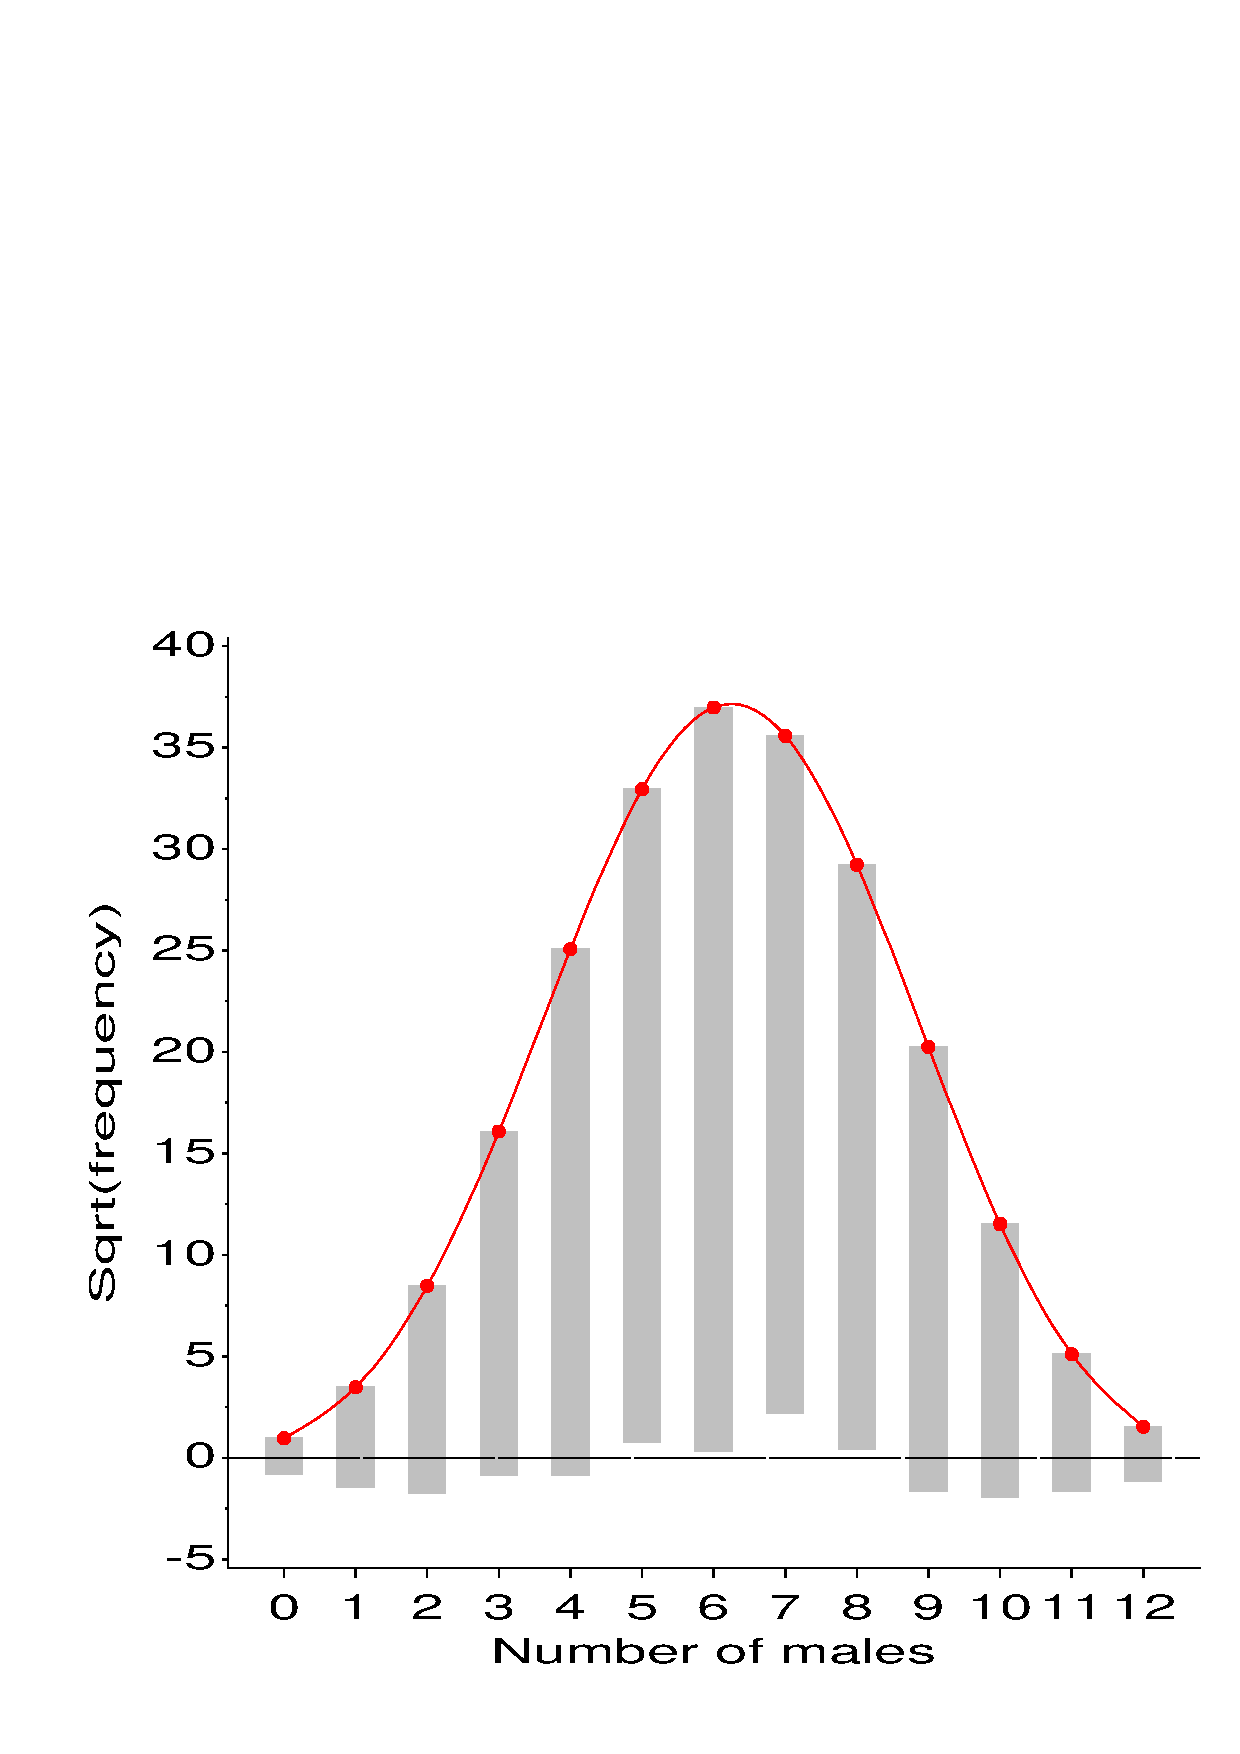
\includegraphics[width=1\linewidth]{saxony}\graphicsfile{ch2/fig/saxony.eps}{}
 \end{minipage}%
 \hfill
 \begin{minipage}[c]{.33\linewidth}
  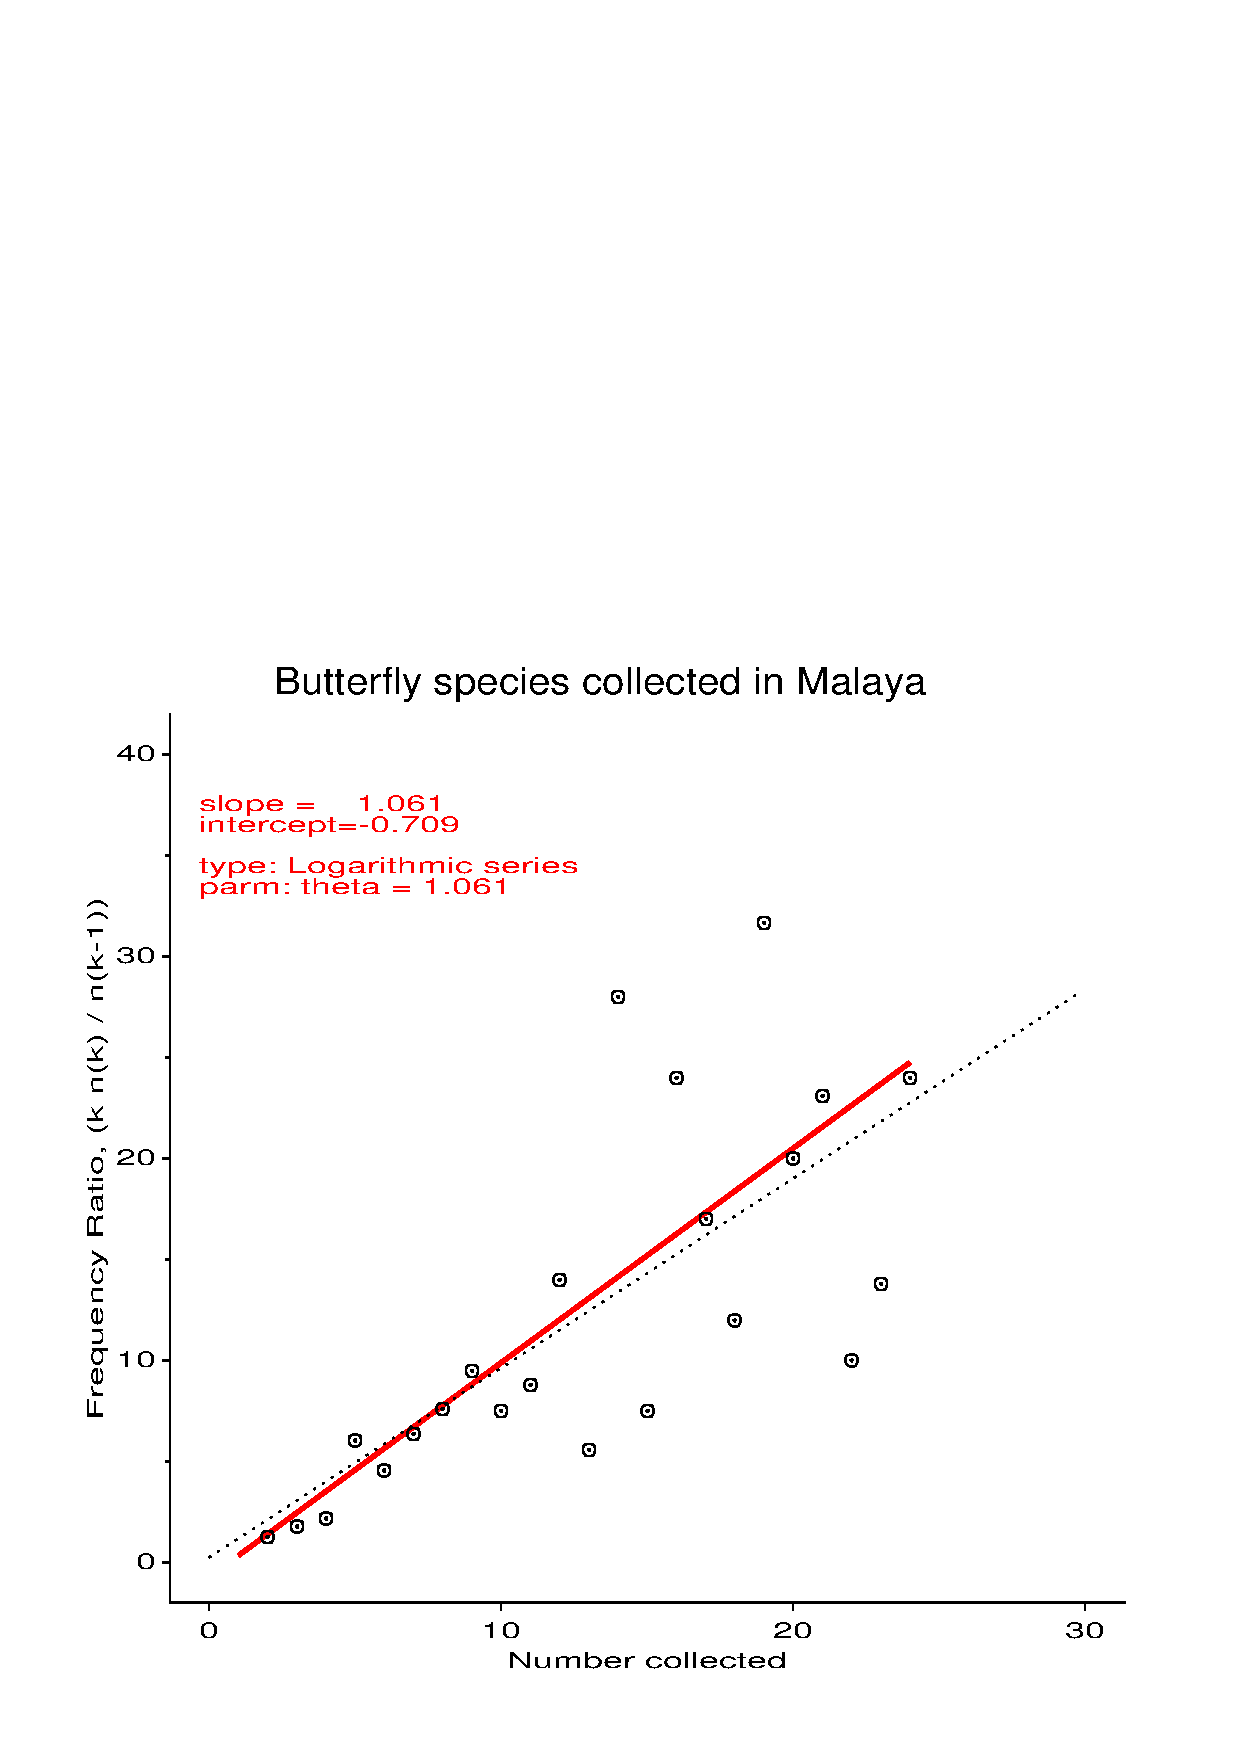
\includegraphics[width=1\linewidth]{orddemo3}\graphicsfile{ch2/fig/orddemo3.eps}{}
 \end{minipage}
 \hfill
 \begin{minipage}[c]{.33\linewidth}
  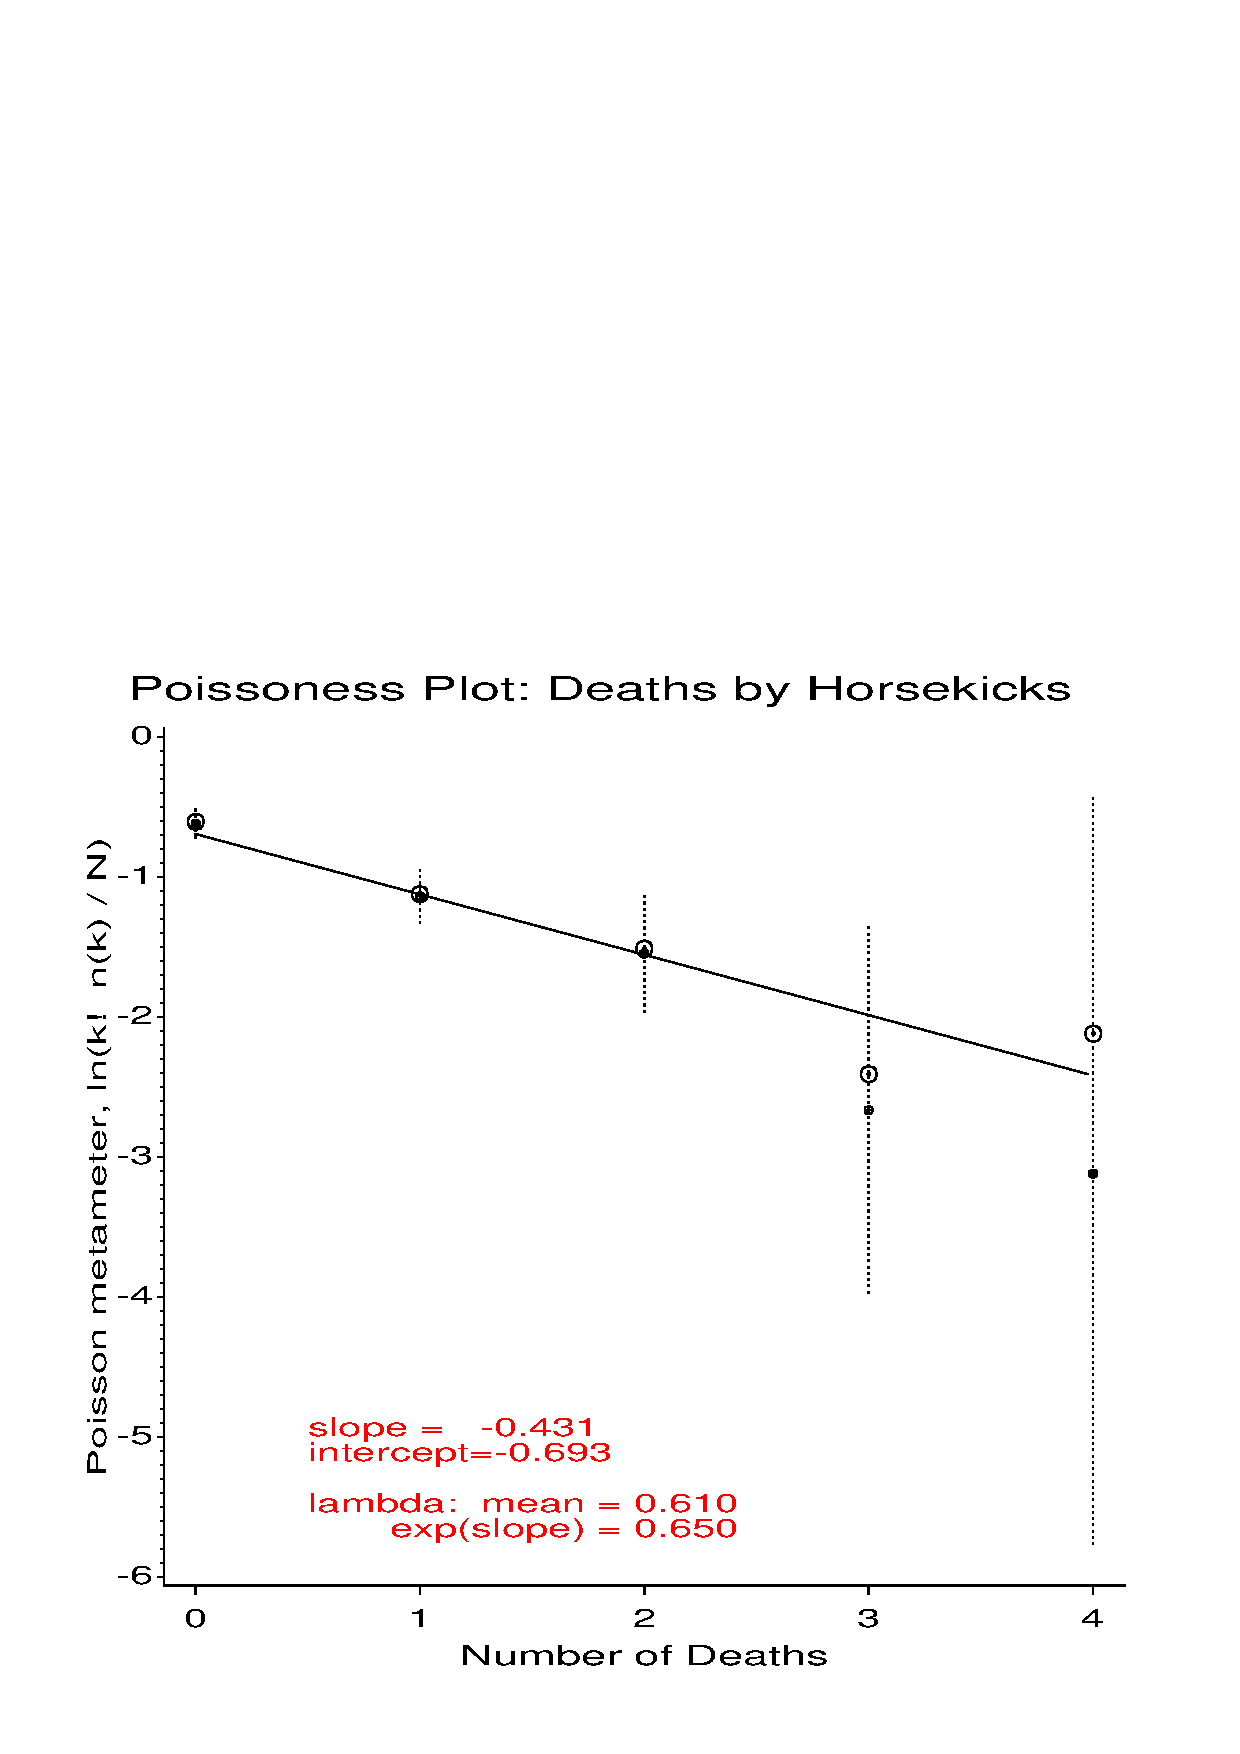
\includegraphics[width=1\linewidth]{poisdemo1}\graphicsfile{ch2/fig/poisdemo1.eps}{}
 \end{minipage}
\end{center}


\begin{quote}
{\Large
Mosaic displays help to visualize the pattern of associations
among variables in two-way and larger tables.  Extensions of
this technique can reveal partial associations, marginal associations,
and shed light on the structure of \loglin\ models themselves. 
}
\end{quote}
\minitoc
\clearpage

\section{Introduction}\label{sec:mosaic-intro}
% \epigraph{Little boxes, on the hillside, little boxes made of ticky-tacky;\\
% Little boxes, little boxes, little boxes all the same.\\
% There's a green one and a pink one and a blue one and a yellow one;\\
% Little boxes, little boxes, and they all look just the same.}%
% {Written and composed by Malvina Renolds, recorded by Pete Seeger}

%\begin{comment}
\epigraph{%
Little boxes on the hillside,
little boxes made of ticky tacky, \\
Little boxes on the hillside,
little boxes all the same. \\
There's a green one and a pink one,
and a blue one and a yellow one, \\
And they're all made out of ticky tacky,
and they all look just the same.
}
{Words and music by Malvina Reynolds, \copyright Schroder Music Company 1962, 1990; recorded by Pete Seeger}
%\end{comment}
In \chref{ch:twoway}, I described a variety of graphical techniques
for visualizing the pattern of association in simple \ctabs{}.
These methods tend to be specialized, however, for particular
shapes and sizes of tables: two-way (sieve diagram),
$2 \times 2$ tables (fourfold display), $r \times 3$ tables
(trilinear plots), and so on.

This chapter describes the
\glossterm{mosaic display},
 a graphical method that displays the
frequencies in a \ctab{} by a collection of rectangular ``tiles''
whose size (area) is proportional to the cell frequency.
In this respect, the mosaic display is similar to the sieve diagram.
The mosaic display, however,

\begin{itemize}
\item generalizes readily to n-way tables.  One can usefully examine
3-way, 4-way and even larger tables, subject, of course, to the limitations
of resolution in any graph;
\item displays the deviations (residuals) from a given log-linear model
which has been fit to the table;
\item provides a method for fitting a series of sequential log-linear
models to the various marginal totals of an n-way table; and
\item can be used to illustrate the relations among variables which
are fitted by various log-linear models.
\end{itemize}

\section{Two-way tables}\label{sec:mosaic-twoway}
The mosaic display 
\citep{Friendly:92b,Friendly:94a,Friendly:97,HartiganKleiner:81,HartiganKleiner:84}
is like a grouped barchart,
where the widths of the bars show the relative frequencies of one
variable, and heights of the sections in each bar show the
relative frequencies of the second variable as shown in \figref{fig:mosaic31}.
% Additional variables can be displayed by dividing 
The construction of the mosaic display, and what it reveals,
are most easily understood for two-way tables.

\begin{Example}[haireye2a]{Hair color and eye color}
Consider the data in \tabref{tab:hairdat},
showing the relation between hair color and eye color among students
in a statistics course.
\begin{figure}[htb]
  \centering
  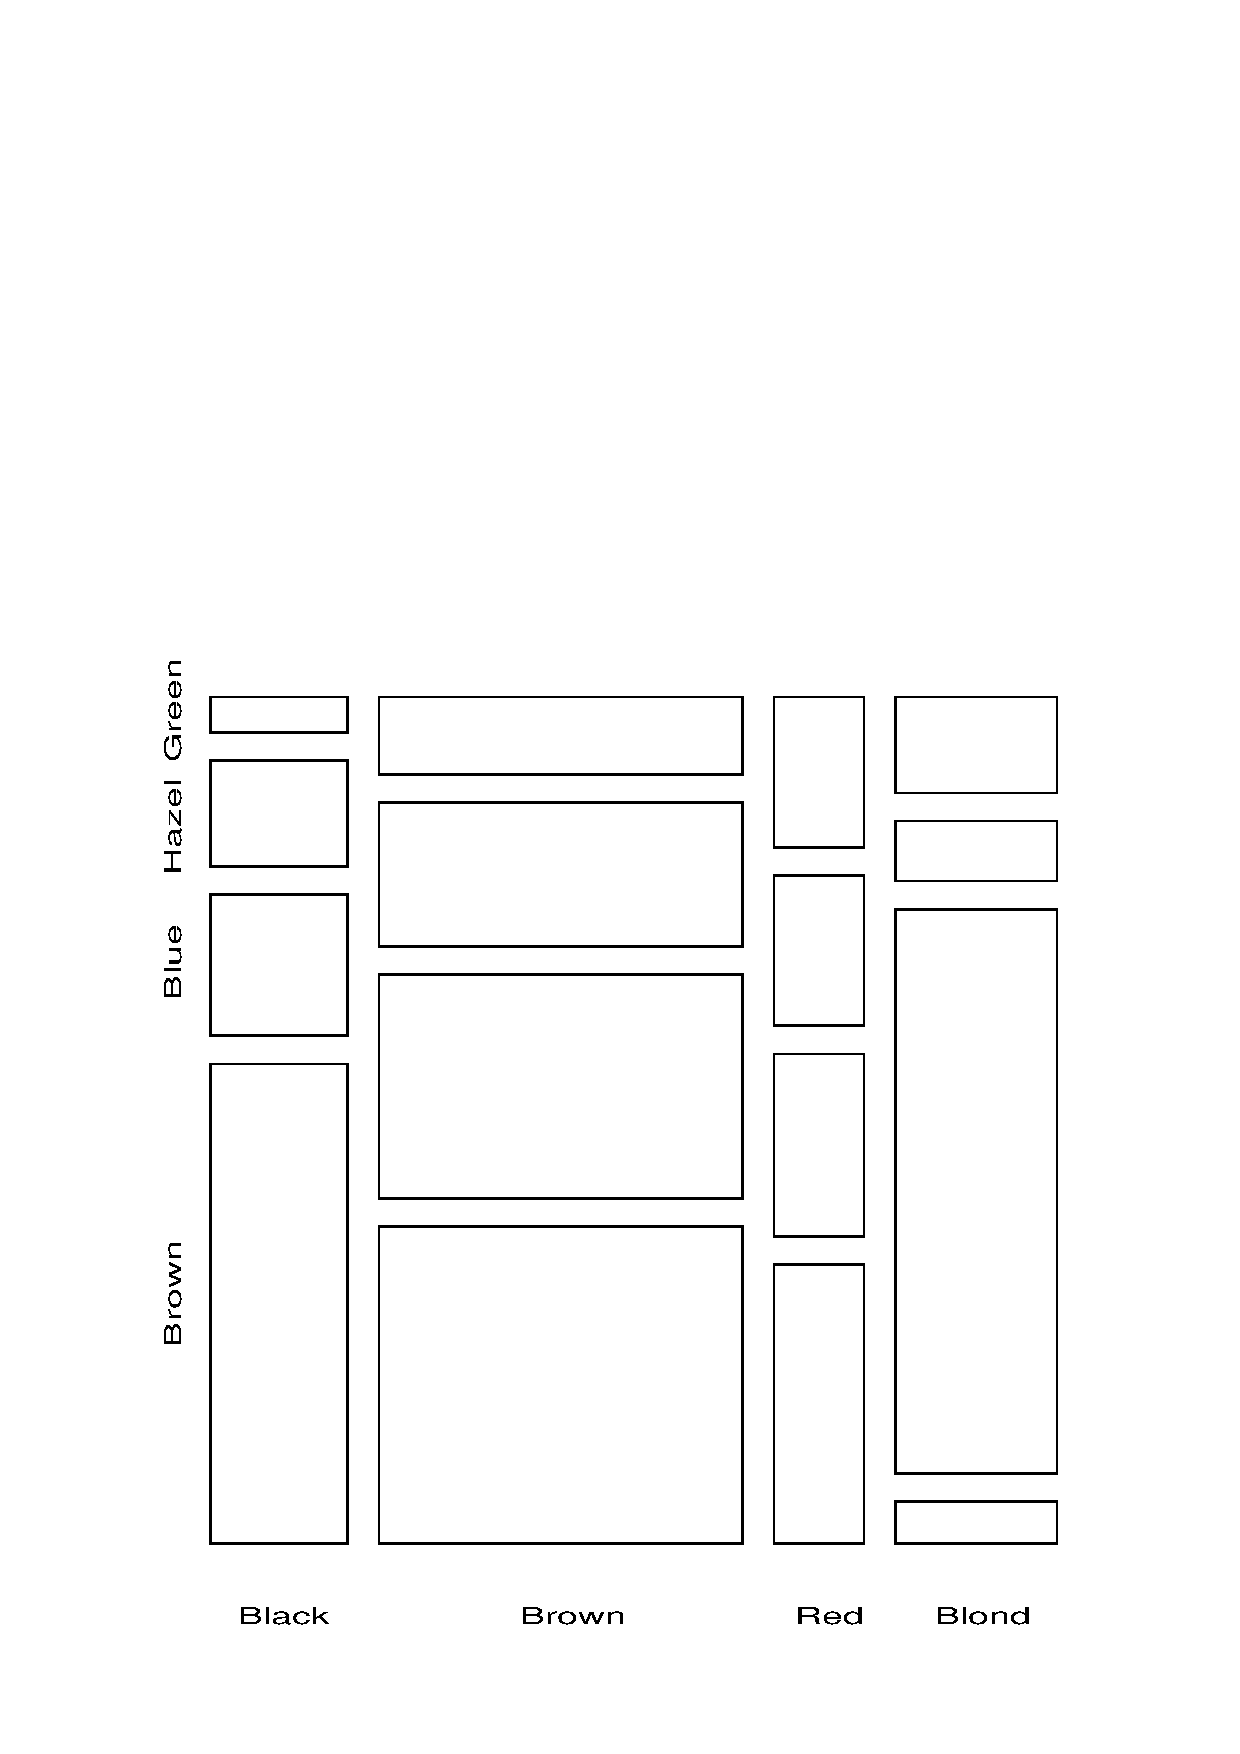
\includegraphics[scale=.6]{ch4/fig/mosaic31}
  \caption[Basic mosaic display for hair color and eye color data]{Basic mosaic display for hair color and eye color data.  The area of each
  rectangle is proportional to the observed frequency in that cell.}%
  \label{fig:mosaic31}
\end{figure}
For such a two-way table, the mosaic display is constructed
by first dividing a unit square in proportion to the marginal
totals of one variable, say, Hair color.

For these data, the marginal frequencies and proportions are:

\begin{minipage}{\linewidth} 
\begin{verbatim} 
              Black      Brown      Red    Blond    TOTAL
Frequencies    108       286        71      127      592
Proportions   0.1824    0.4831    0.1199   0.2145   1.000
\end{verbatim}
\end{minipage}


These can be shown as the mosaic for the first variable (hair color),
as in \figref{fig:mosaic32}.
The rectangular tiles are shaded to show the residuals (deviations)
from a particular model, as follows:
\begin{figure}[htb]
  \centering
  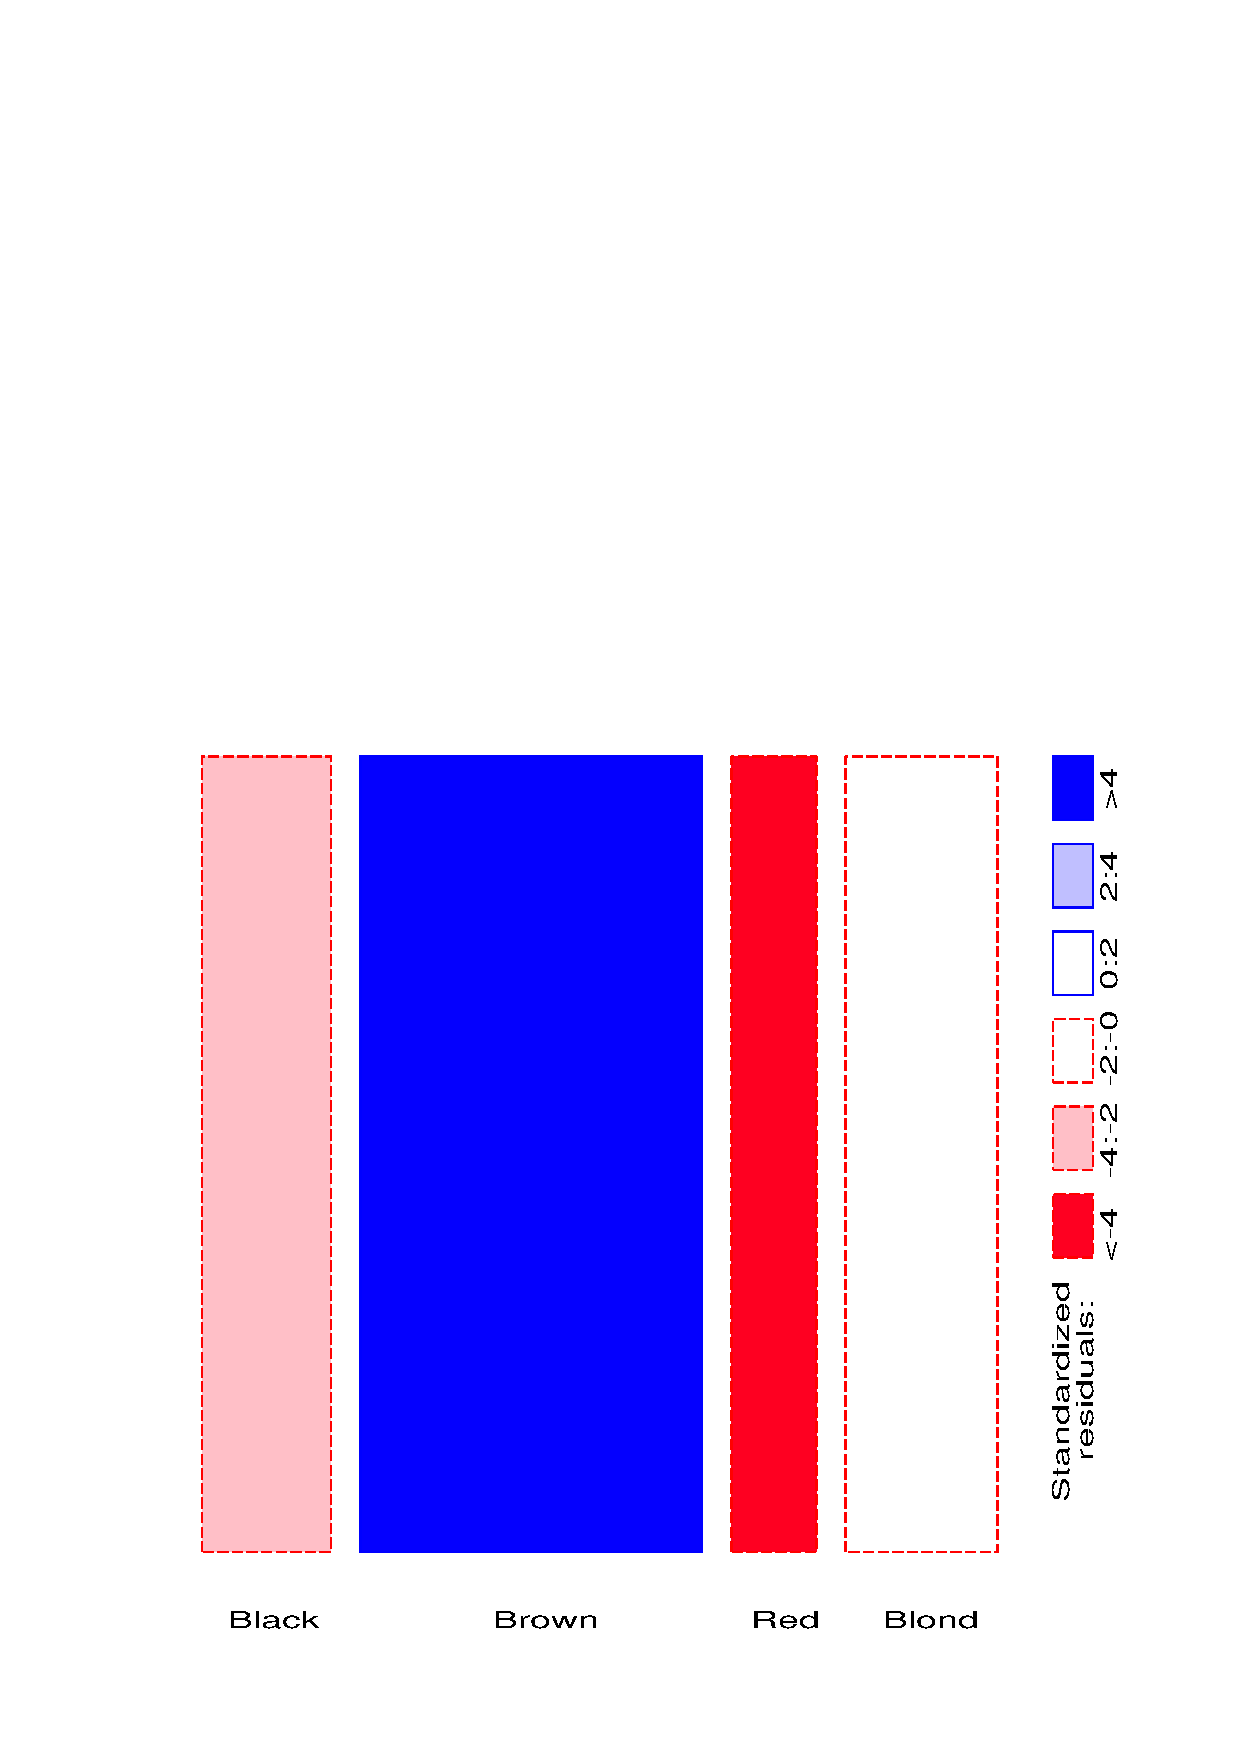
\includegraphics[scale=.6]{ch4/fig/mosaic32}
  \caption{First step in the mosaic display}%
  \label{fig:mosaic32}
\end{figure}

\begin{itemize}
\item The one-way table of marginal totals can be fit to a model, in this
case, the model that all hair colors are equally probable.  This model
has expected frequencies $m_i = 592/4$:
\begin{verbatim} 
               Fitted frequencies
       Black      Brown      Red    Blond
       148.00    148.00    148.00   148.00
\end{verbatim}
\item The Pearson residuals from this model, $d_i = ( n_i - m_i ) / \sqrt{m_i}$, are:
\begin{verbatim} 
         Standardized Pearson residuals
       Black    Brown      Red    Blond
       -3.29    11.34    -6.33    -1.73
\end{verbatim}
and these values are shown by color and shading as shown in the legend.
The high positive value for Brown hair indicates that people
with brown hair are much more frequent in this sample than 
the Equiprobability model would predict.
\end{itemize}

Next, the rectangle for each Hair color is subdivided in proportion
to the relative (conditional) frequencies of the second variable --
Eye color, giving the following conditional proportions:
\begin{verbatim} 
                     Marginal proportions
                Brown     Blue    Hazel    Green   TOTAL

      Black    0.6296   0.1852   0.1389   0.0463    1.0
      Brown    0.4161   0.2937   0.1888   0.1014    1.0
      Red      0.3662   0.2394   0.1972   0.1972    1.0
      Blond    0.0551   0.7402   0.0787   0.1260    1.0
\end{verbatim}
The proportions in each row determine the heights of the tiles in the second mosaic display in \figref{fig:mosaic33}.
\begin{figure}[htb]
  \centering
  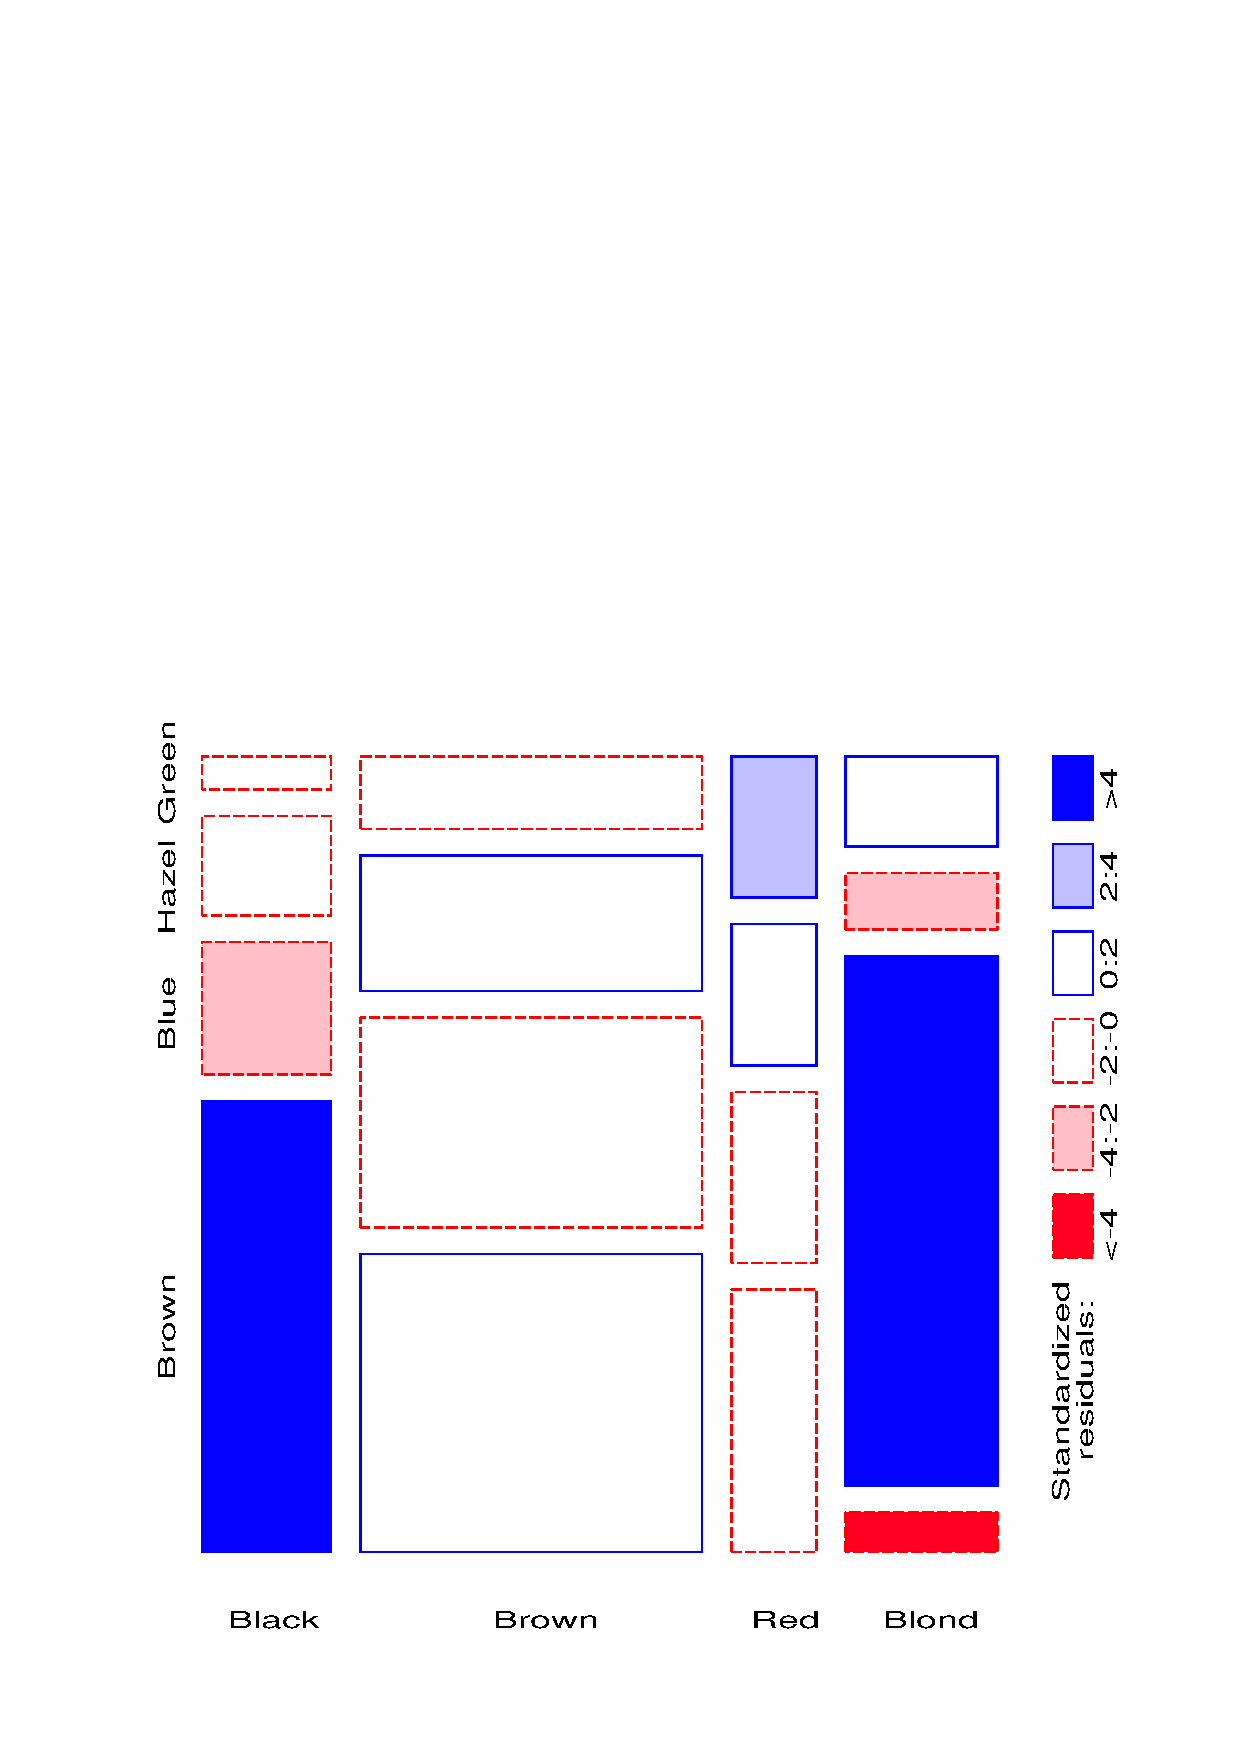
\includegraphics[scale=.6]{ch4/fig/mosaic33}
  \caption[Second step in the mosaic display]{Second step in the mosaic display.  Each rectangle for hair color is subdivided in proportion to the
  frequencies of eye color.}%
  \label{fig:mosaic33}
\end{figure}

\begin{itemize}
\item Again, the cells are shaded in relation to standardized
residuals, \(d_{ij} = (
n_{ij} - m_{ij}) / \sqrt { m_{ij} }\), 
from a model.  For a two-way table, the model is that Hair color and
Eye color are independent in the population from which this sample
was drawn.
\begin{verbatim} 
               Standardized Pearson residuals
               Brown     Blue    Hazel    Green

      Black     4.40    -3.07    -0.48    -1.95
      Brown     1.23    -1.95     1.35    -0.35
      Red      -0.07    -1.73     0.85     2.28
      Blond    -5.85     7.05    -2.23     0.61
\end{verbatim}
\item Thus, the two tiles shaded deep blue correspond to the two
cells, (Black, Brown) and (Blond, Blue), whose residuals are
greater than $+4$, indicating much greater frequency in those
cells than would be found if Hair color and Eye color were
independent.
The tile shaded deep red, (Blond, Brown)
corresponds to the largest residual = -5.85, indicating this combination
is extremely rare under the hypothesis of independence.
\item The overall Pearson \chisq{} statistic is just the
sum of squares of the residuals.
\end{itemize}
\end{Example}

\subsubsection{Shading levels}

The default shading patterns for the tiles are based on standardized
residuals which exceed the values 2 and 4 in absolute value.%
\footnote{In \Dset{}s with very large total frequency,
most models may fit poorly and have large residuals.
In such cases (e.g., \exref{ex:suicide1}) it is often useful to define
more shading levels to make finer distinctions.  For example,
in \exref{ex:suicide1} we use \pname{SHADE=\{2 4 8\};} to set
three levels of shading.}
Since the standardized residuals are approximately unit-normal $N(0,1)$
values,  this corresponds to highlighting cells whose
residuals are \emph{individually} significant at approximately
the .05 and .0001 level, respectively.
The purpose of highlighting cells, however, is not to provide tests
of significance, but rather to draw attention to the \emph{pattern}
of departures of the data from the assumed model.
In any case, 
the number and values of
these cutoffs can be easily set by the user using the \pname{SHADE}
parameter.

To provide some redundancy when color figures are reproduced in 
black and white, cells with positive residuals are outline with solid
(blue) lines, while cells with negative residuals are outlined with broken
(red) lines.
Cells whose absolute residuals are less than the smallest shading level
are unfilled.  For good-fitting models, it is sometimes useful to distinguish
between near-zero residuals and small, non-significant residuals.
In color figures, near-zero cells are outlined in solid black;
the threshold is determined by the \pname{FUZZ} parameter.

\subsubsection{Interpretation}

To interpret the association between Hair color and Eye color,
consider the pattern of positive (Blue) and negative (Red)
tiles in the mosaic display.  
We interpret positive values as showing cells whose observed frequency
is substantially greater than would be found under independence;
negative values indicate cells which occur less often than
under independence.

\ixe{Hair color and eye color|(}
This interpretation is enhanced by reordering the rows or columns
of the two-way table so that the residuals have an opposite
corner pattern of signs.  This usually helps us interpret any systematic
patterns of association in terms of the ordering of the row and column
categories.
Here, this is achieved by reordering the Eye colors as shown in
\figref{fig:mosaic34},  and we note that in this rearrangement
both hair colors and eye colors are ordered from dark to light.
(In general, the levels of a factor may be reordered by
arranging them according to their scores on the first (largest)
correspondence analysis dimension; see
\citep{Friendly:94a}).
The re-ordered residuals are:
\begin{verbatim} 
         Standardized Pearson residuals

          Brown    Hazel    Green     Blue

Black      4.40    -0.48    -1.95    -3.07
Brown      1.23     1.35    -0.35    -1.95
Red       -0.07     0.85     2.28    -1.73
Blond     -5.85    -2.23     0.61     7.05
\end{verbatim}
\begin{figure}[htb]
  \centering
  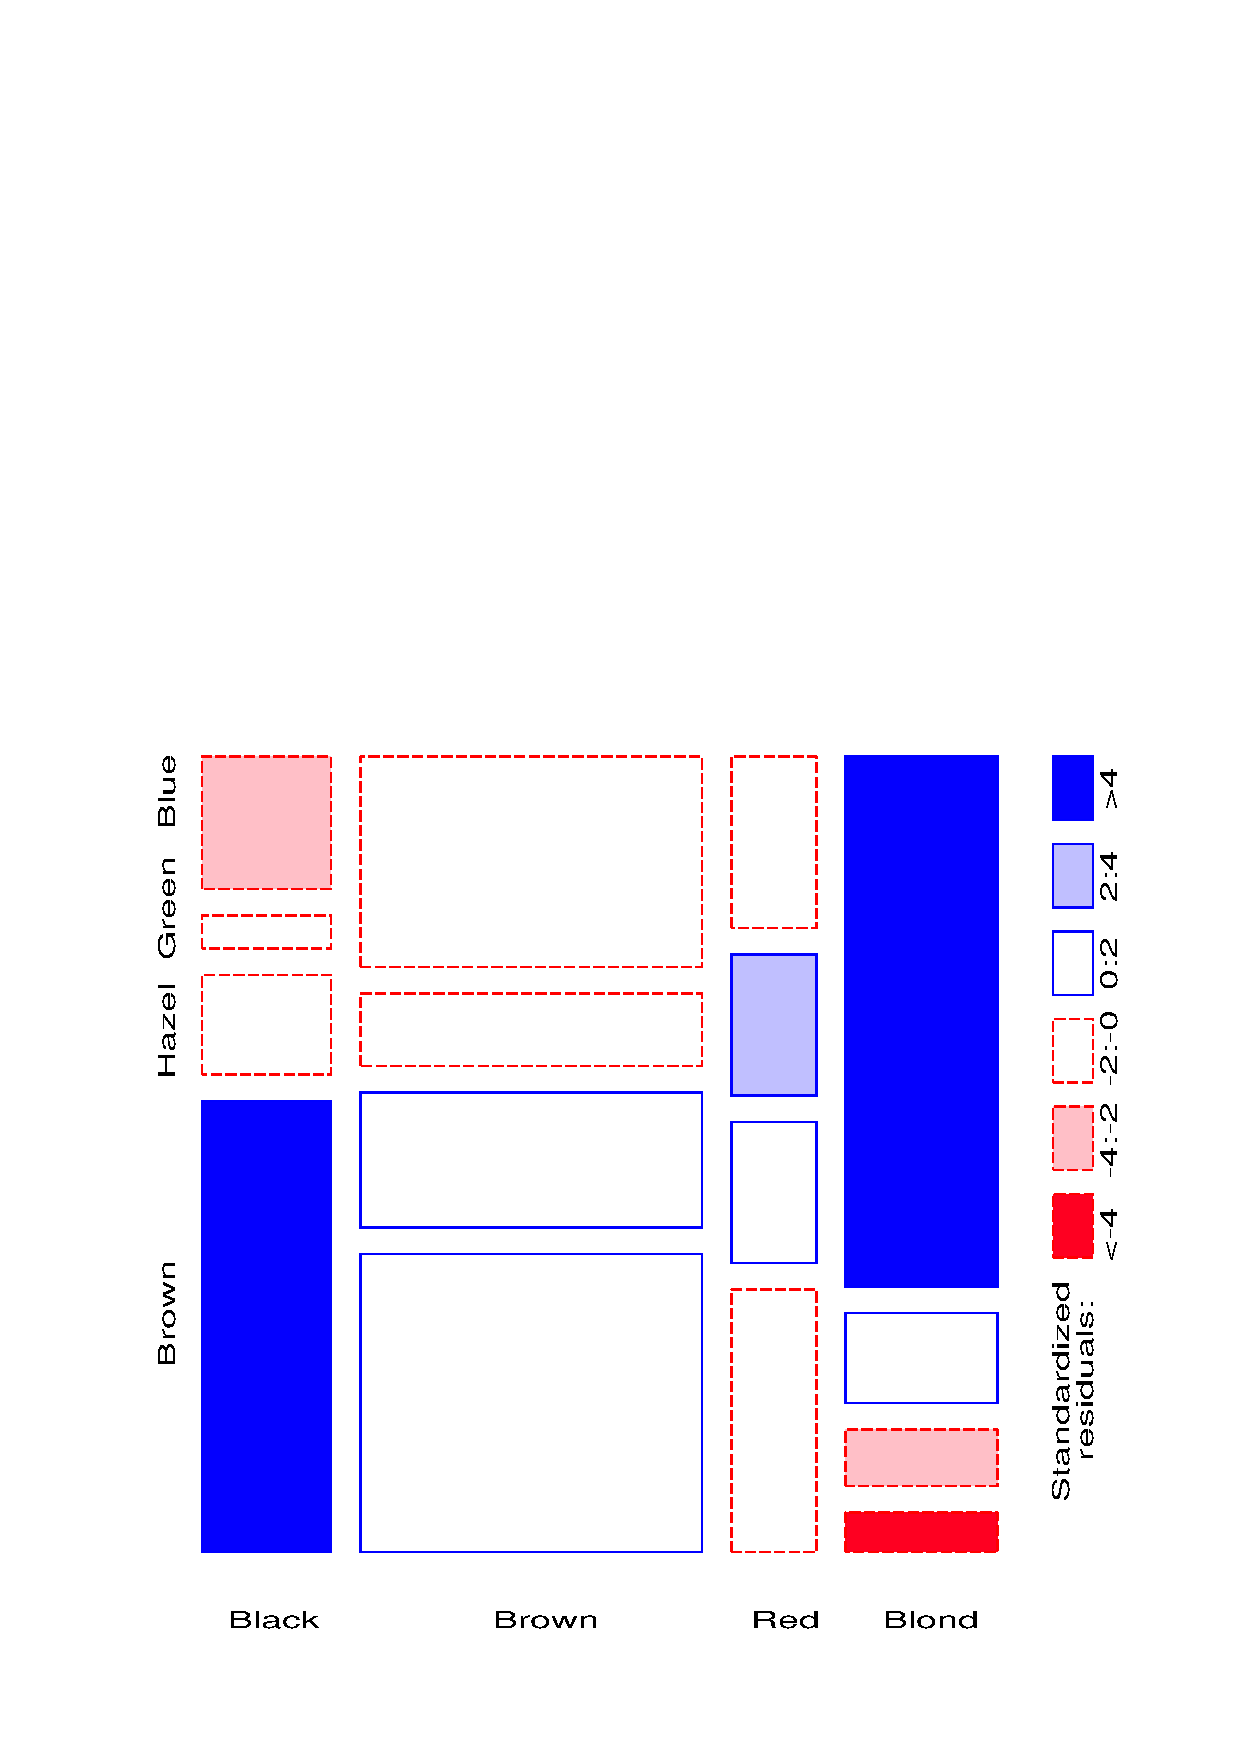
\includegraphics[scale=.6]{ch4/fig/mosaic34}
  \caption[Two-way mosaic, reordered]{Two-way mosaic,
  reordered.  Deviations from independence are shown by
  color and shading.  The two levels of shading density correspond to
  standardized deviations greater than 2 and 4 in absolute value.
  This form of the display generalizes readily to multi-way
  tables.}  \label{fig:mosaic34}
\end{figure}
Thus, the mosaic shows that the association between Hair and Eye color
is essentially that 
\begin{itemize*}
\item people with dark hair tend to have dark eyes,
\item those with light hair tend to have light eyes
\item people with red hair do not quite fit this pattern
\end{itemize*}
\ixe{Hair color and eye color|)}

\subsection{Software for mosaic displays}
Mosaic displays are implemented as a collection of modules
(the \sasprog{mosaics.sas}) written in \IML{},
which are used within a \PROC{IML} step,
as described in \macref{mac:mosaics}.  The program is designed so that
the frequency table, and its associated factor levels and variable names
may be entered directly using \IML{} statements,
or (using the \module{readtab}) may be input from a SAS \Dset\
of the form produced by \PROC{FREQ}.
Using the \sasprog{mosaics.sas} within a \PROC{IML} step is most
flexible, because you can use \IML{} statements and modules within
\texttt{mosaics.sas} to manipulate the frequency table (selecting
or reordering rows or columns), to specify structural zeros,
or to fit specialized models which cannot be fit by other means.

In addition, several SAS macros
are provided to simplify the use of \texttt{mosaics.sas}. 
The \macro{MOSAIC} (described in \macref{mac:mosaic})
may be used with any SAS \Dset\ in frequency
form (e.g., the output from \PROC{FREQ}).  It reads the data into
\IML{} and provides basic mosaic displays,
mosaics for externally-calculated residuals,
and partial mosaic displays (\secref{sec:mospart}).
The \macro{TABLE} (\macref{mac:table}) may be used to construct the frequency table, and
to collapse or recode variables.
The \macro{MOSMAT} (\macref{mac:mosmat})
provides mosaic matrices (\secref{sec:mosmat}),
an analog of the \scatmat{} for categorical data.

Two examples below illustrate the use of this software for basic mosaic
displays.
\exref{ex:soccer2} uses the \macro{MOSAIC},
while \exref{ex:victims}
uses \PROC{IML} statements to construct and manipulate the
frequency table.

\begin{table}[!hb]
\caption{Total goals scored in 380 games in the Premier
Football League, 1995/95 season}
\label{tab:soccer2}
\vspace{.1in}
\begin{center}
\begin{tabular}{l|rrrr rrrr}
\hline
Total goals      &  0  &  1  &  2  &  3  &  4  &  5  &  6  &  7  \\
\hline
Number of games  & 27  & 88  & 91  & 73  & 49  & 31  & 18  &  3  \\
  \hline
\end{tabular}
\end{center}
\end{table}

%%
% Table victims written by md2tex  1-29-1998
\begin{table}[htb]
 \caption{Repeat Victimization Data}
 \label{tab:victims}
 \begin{center}
  \begin{tabular}{|l|rrrrrrrr|}
   \hline
 & \multicolumn{8}{c|}{\bfseries\large First Victimization }\rule{0in}{2.5ex}\\
{\bfseries\large Second       } &          &       &       & Pick     & Personal &      & Household & Auto    \\
{\bfseries\large Victimization} & Rape     & Assault & Robbery & Pocket & Larceny & Burglary & Larceny & Theft   \\
   \hline
% f=        2 t=        1
Rape                   &            26 &            65 &            12 &             3 &            75 &            52 &            42 &             3 \\
Assault                &            50 &          2997 &           279 &           102 &          2628 &          1117 &          1251 &           221 \\
Robbery                &            11 &           238 &           197 &            40 &           413 &           191 &           206 &            51 \\
Pick Pocket            &             6 &            85 &            36 &            61 &           329 &           102 &           117 &            24 \\
Personal Larceny           &            82 &          2553 &           459 &           243 &         12137 &          2649 &          3757 &           678 \\
Burglary               &            39 &          1083 &           197 &           115 &          2658 &          3210 &          1962 &           301 \\
Household Larceny           &            48 &          1349 &           221 &           101 &          3689 &          1973 &          4646 &           367 \\
Auto Theft             &            11 &           216 &            47 &            38 &           687 &           301 &           391 &           269 \\
   \hline
  \end{tabular}
 \end{center}
\end{table}


\section{Three-way tables}\label{sec:mosaic-threeway}

The mosaic display can be extended to three- and higher-way tables.
The relative frequencies of a third variable are used to subdivide
each two-way cell, and so on, recursively.

Imagine that each
cell of the two-way table for Hair and Eye color is further
classified by one or more additional variables---sex and level of
education, for example.  Then each rectangle can be subdivided
horizontally to show the proportion of males and females in that
cell, and each of those horizontal portions can be subdivided
vertically to show the proportions of people at each educational
level in the hair-eye-sex group.

\figref{fig:mosaic35} shows the mosaic for the three-way table, with Hair and Eye color
groups divided according to the proportions of Males and Females:
We see that there is no systematic association between sex
and the combinations of Hair and Eye color---except among
blue-eyed blonds, where there are an overabundance of females.

\begin{figure}[!htb]
  \centering
  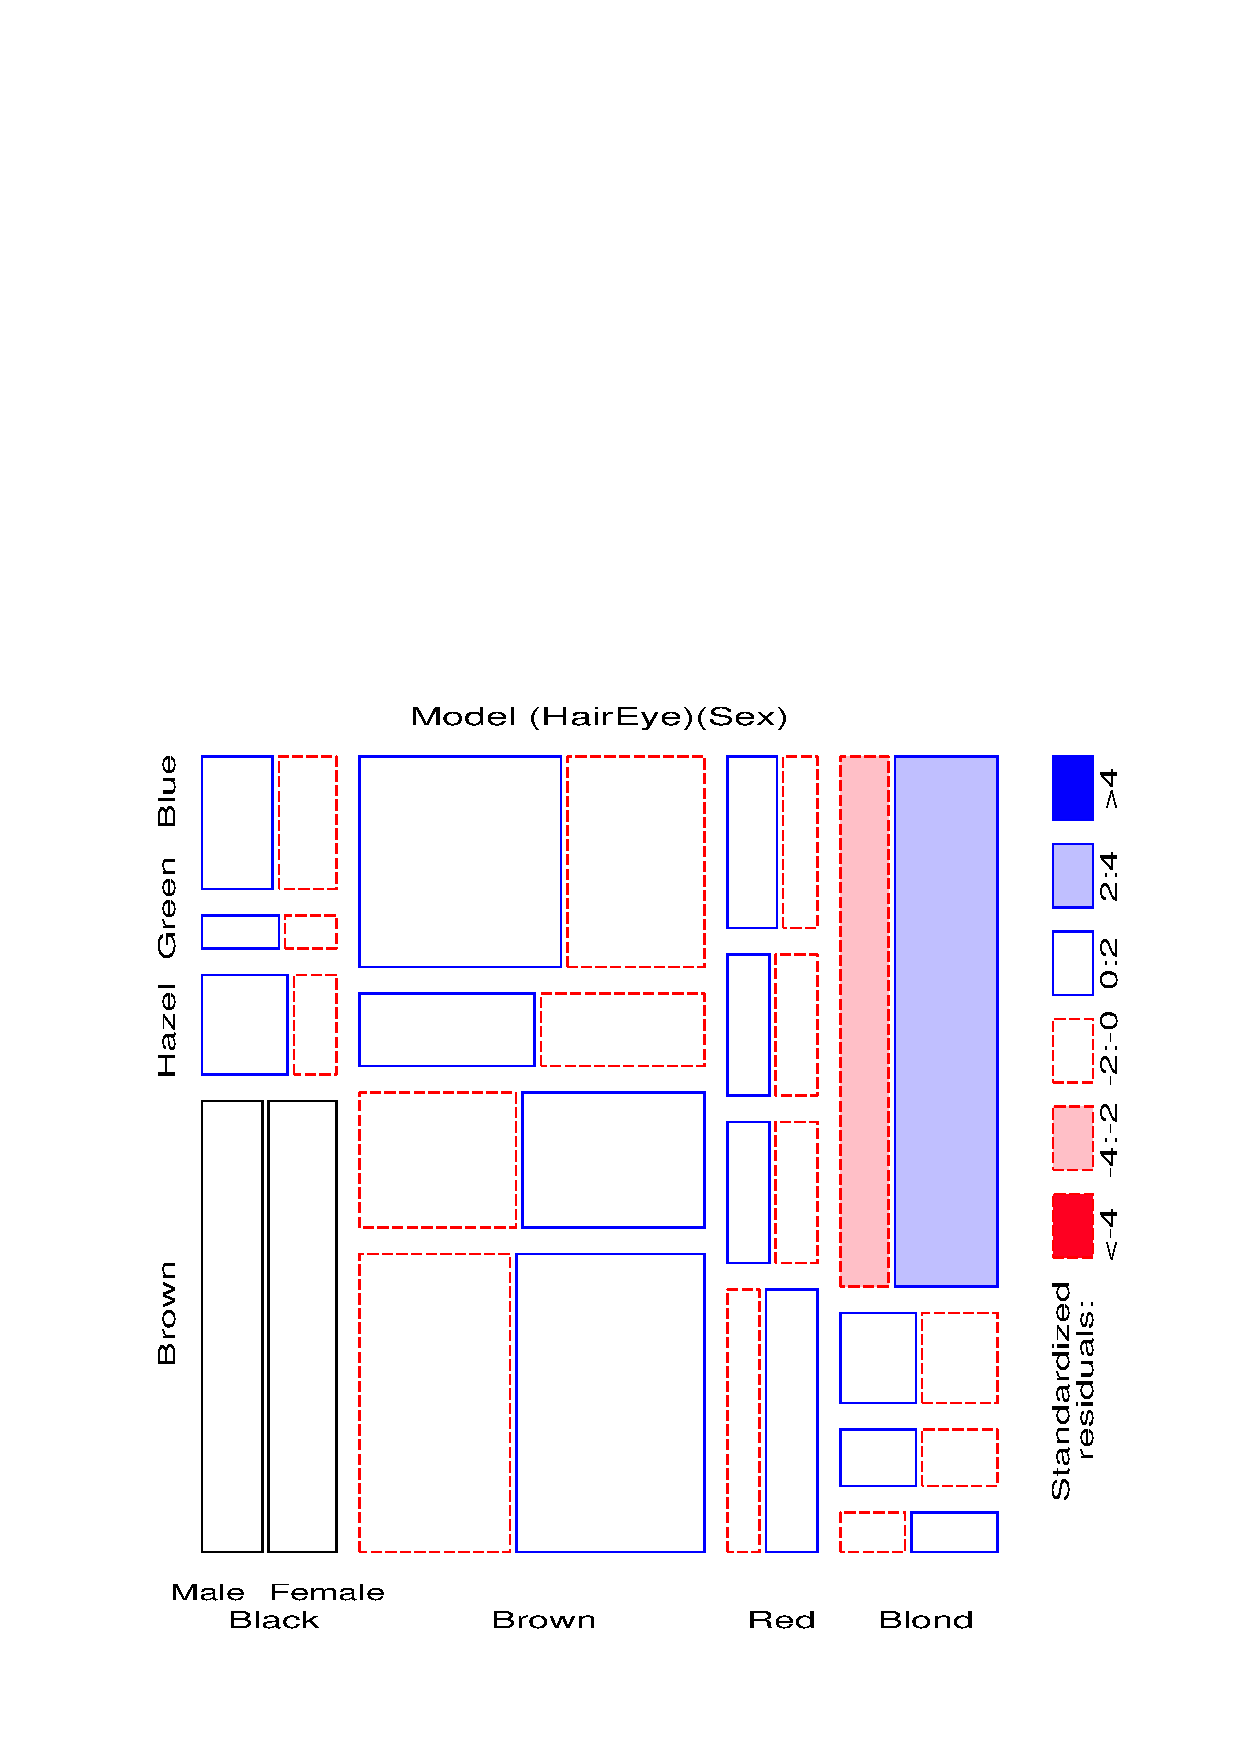
\includegraphics[scale=.6]{ch4/fig/mosaic35}
  \caption[Three-way mosaic, joint independence]{Three-way mosaic display for hair color, eye
color, and sex.
The categories of sex are crossed with those of
hair color, but only the first occurrence is labeled.
Residuals from
the model of joint independence, \([HE]\,  [S]\) are shown by
shading.
\(G^2\) = 19.86 on 15 df.
The only lack of fit is
an overabundance of females among blue-eyed blonds.}
\label{fig:mosaic35}
\end{figure}

\subsection{Fitting models}\label{sec:mosaic-fitting}
When three or more variables are
represented in the mosaic, we can fit several different models of
``independence'' and display the residuals from each model.  We treat
these models as null or baseline models, which may not fit the data
particularly well.  The deviations of observed frequencies from
expected ones, displayed by shading, will often suggest terms to be added
to an explanatory model that achieves a better fit.

For a three-way table, with variables $A$, $B$ and $C$, some of the hypothesized models which can be fit are
described below and summarized in \tabref{tab:hyp3way}.
Here I use $[\,]$ notation to list the \emph{high-order terms} in
a hierarchical \loglin{} model; these correspond to the margins
of the table which are fitted exactly.  The notation \LLM{AB,AC},
for example, is shorthand for the model
\begin{equation*}
  \log \,  m_{ijk}  =
  \mu  +  \lambda_i^A
  +  \lambda_j^B
  +  \lambda_k^C
  +  \lambda_{ij}^{AB}
  +  \lambda_{ik}^{AC}
  \comma
\end{equation*}
as described in \secref{sec:loglin-counts}, and reproduces the
$\{AB\}$ and $\{AC\}$ marginal subtables.
Here, $A \perp B$ is
read, ``$A$ is independent of $B$.''  \tabref{tab:hyp3way} also
depicts the relations among variables as an
association graph, where associated variables are connected by an edge.

Each model fits certain table margins exactly, as shown in the table;
other associations present in the data will appear in the pattern of
residuals.
\begin{description}
\item[$H_1$: Complete independence.]  The model of complete (mutual) independence, symbolized $A \perp B \perp C$,
       asserts that all joint probabilities are products of the
       one-way marginal probabilities:
\begin{equation*}
 \pi_{ijk} = \pi_{i++} \: \pi_{+j+} \: \pi_{++k}
 \comma
\end{equation*}
for all \(i , j , k\) in a
       three-way table.  This corresponds to the log-linear model
       \LLM{A,B,C}.  Fitting this model puts all higher
       terms, and hence all association among the variables, into the
       residuals.
\item[$H_2$: Joint independence.]  Another possibility is to fit the model in
       which variable \(C\) is jointly independent of variables \(A\)
       and \(B\), ($A , B \perp C $), where
\begin{equation*}
 \pi_{ijk}  =  \pi_{ij+} \:  \pi_{++k} \period
\end{equation*}
This corresponds to the log-linear model \LLM{AB,C}.
Residuals from this model show the extent to which
variable \(C\) is related to the combinations of variables
\(A\) and \(B\) but they do not show any association between
\(A\) and \(B\), since that association is fitted exactly.
For this model, variable $C$ is also independent of $A$ and
$B$ in the marginal $\{AC\}$ table (collapsing over $B$) and
in the marginal $\{BC\}$.

\item[$H_3$: Conditional independence.] Two variables, say $A$ and $B$ are conditionally independent
given the third ($C$) if $A$ and $B$ are independent when we
control for $C$, symbolized as $A \perp B \given C$.
This means that conditional probabilities, $\pi_{ij|k}$ obey
\begin{equation*}
 \pi_{ij|k}  =  \pi_{i+|k} \:  \pi_{+j|k} \comma
\end{equation*}
where
$\pi_{ij|k} = \pi_{ijk} / \pi_{ij+}$,
$\pi_{i+|k} = \pi_{i+k} / \pi_{i++}$, and
$\pi_{+j|k} = \pi_{+jk} / \pi_{+j+}$.
The corresponding \loglin{} models is denoted \LLM{AC,BC}.
When this model is fit, the mosaic display shows the conditional
associations between variables $A$ and $B$, controlling for $C$,
but does not show the associations between $A$ and $C$, or
$B$ and $C$.

\item[$H_4$: No three-way interaction.]  For this model, no pair is
marginally or
conditionally independent, so there is \emph{no} independence interpretation.
Nor is there a closed-form expression for the cell probabilities.
However, the association between any two
variables is the same at each level of the third variable.
The corresponding \loglin{} model formula is \LLM{AB,AC,BC},
indicating that all two-way margins are fit exactly and so are not
shown in the mosaic residuals.
\end{description}
\begin{comment}
\newcommand{\tridot}[1]{%
	\begin{pspicture}(-.01, -.01)(1.1,1.1)%
	\psset{xunit=.85cm,yunit=.85cm}%
	\color{black}%
	\rput(0,0){\circlenode{A}{\textsf{A}}}%
	\rput(1.0,0){\circlenode{B}{\textsf{B}}}%
	\rput(.5,.866){\circlenode{C}{\textsf{C}}}%
	#1%
	\end{pspicture}%
	\rule{0in}{1.2cm}
%	}
}
\end{comment}

\newcommand{\tridot}[1]{%
\begin{tikzpicture}[x=0.9cm, y=0.9cm]
  \node(A)[draw, circle, fill=yellow!30,scale=0.9] at (0,0) {\textbf{\textsf{A}}};
  \node(B)[draw, circle, fill=yellow!30,scale=0.9] at (1,0) {\textbf{\textsf{B}}};
  \node(C)[draw, circle, fill=yellow!30,scale=0.9] at (.5,.866) {\textbf{\textsf{C}}};
  #1%
%  \path (A) edge (B);
%  \path (B) edge (C);
%  \draw (0,0) circle 
\end{tikzpicture}
}


\begin{table}[htb]
\caption[Hypotheses for a three-way table]{Fitted margins, model symbols and interpretations for some hypotheses for a three-way table.}\label{tab:hyp3way}
\begin{center}
  \begin{tabular}{|clllc|} \hline
  \tableheader
  Hypothesis & \multilineC{Fitted\\margins} & \multilineC{Model\\symbol} & \multilineC{Independence\\interpretation} & \multilineC{Association\\graph} \\
%             & Fitted  & Model &  Independence  & Association  \\
%  Hypothesis & margins & symbol & Interpretation & graph \\
   \hline 
  $H_1$ & $n_{i++}, n_{+j+}, n_{++k}$ & [A][B][C] & $A \perp B \perp C $ & 
  \tridot{} \\[3ex] 
  $H_2$ & $n_{ij+}, n_{++k}$ & [AB][C] & $(A , B )\perp C $ & 
  \tridot{\path (A) edge (B);} \\[3ex]
%
  $H_3$ & $n_{i+k}, n_{+jk}$ & [AC][BC] & $A \perp B \: |\: C$ & 
  \tridot{\path (A) edge (C); \path (B) edge (C);} \\[3ex]
  $H_4$ & $n_{ij+}, n_{i+k}, n_{+jk}$ & [AB][AC][BC] & \texttt{NA} & 
  \tridot{\path (A) edge (B); \path (B) edge (C); \path (A) edge (C);} \\[3ex]
%
  \hline
  \end{tabular}
 \end{center}
\end{table}



For example, with the data from \tabref{tab:hairdat} broken down
by sex, fitting the joint-independence model [HairEye][Sex] allows us to see the extent
to which the joint distribution of hair color and eye color is
associated with sex.  For this model, the likelihood-ratio \(G^2\) is
19.86 on 15 \(df\) (\(p  =  .178\)), indicating an acceptable overall fit.
The three-way mosaic for this model was shown in \figref{fig:mosaic35}.
Any other model fit to this table will have the same size tiles in the mosaic
since the areas depend on the observed frequencies;  the residuals,
and hence the shading of the tiles will differ.
Thus, fitting a conditional independence model, [HairSex][EyeSex]
would test whether, given sex, hair color and eye color are independent
(probably not a meaningful hypothesis, here).
This model fits very poorly ($G^2 (18) = 156.68$).
The mosaic display, shown in \figref{fig:mosaic36}, has a pattern
similar to that in the two-way display, \figref{fig:mosaic34}.

\begin{figure}[!htb]
  \centering
  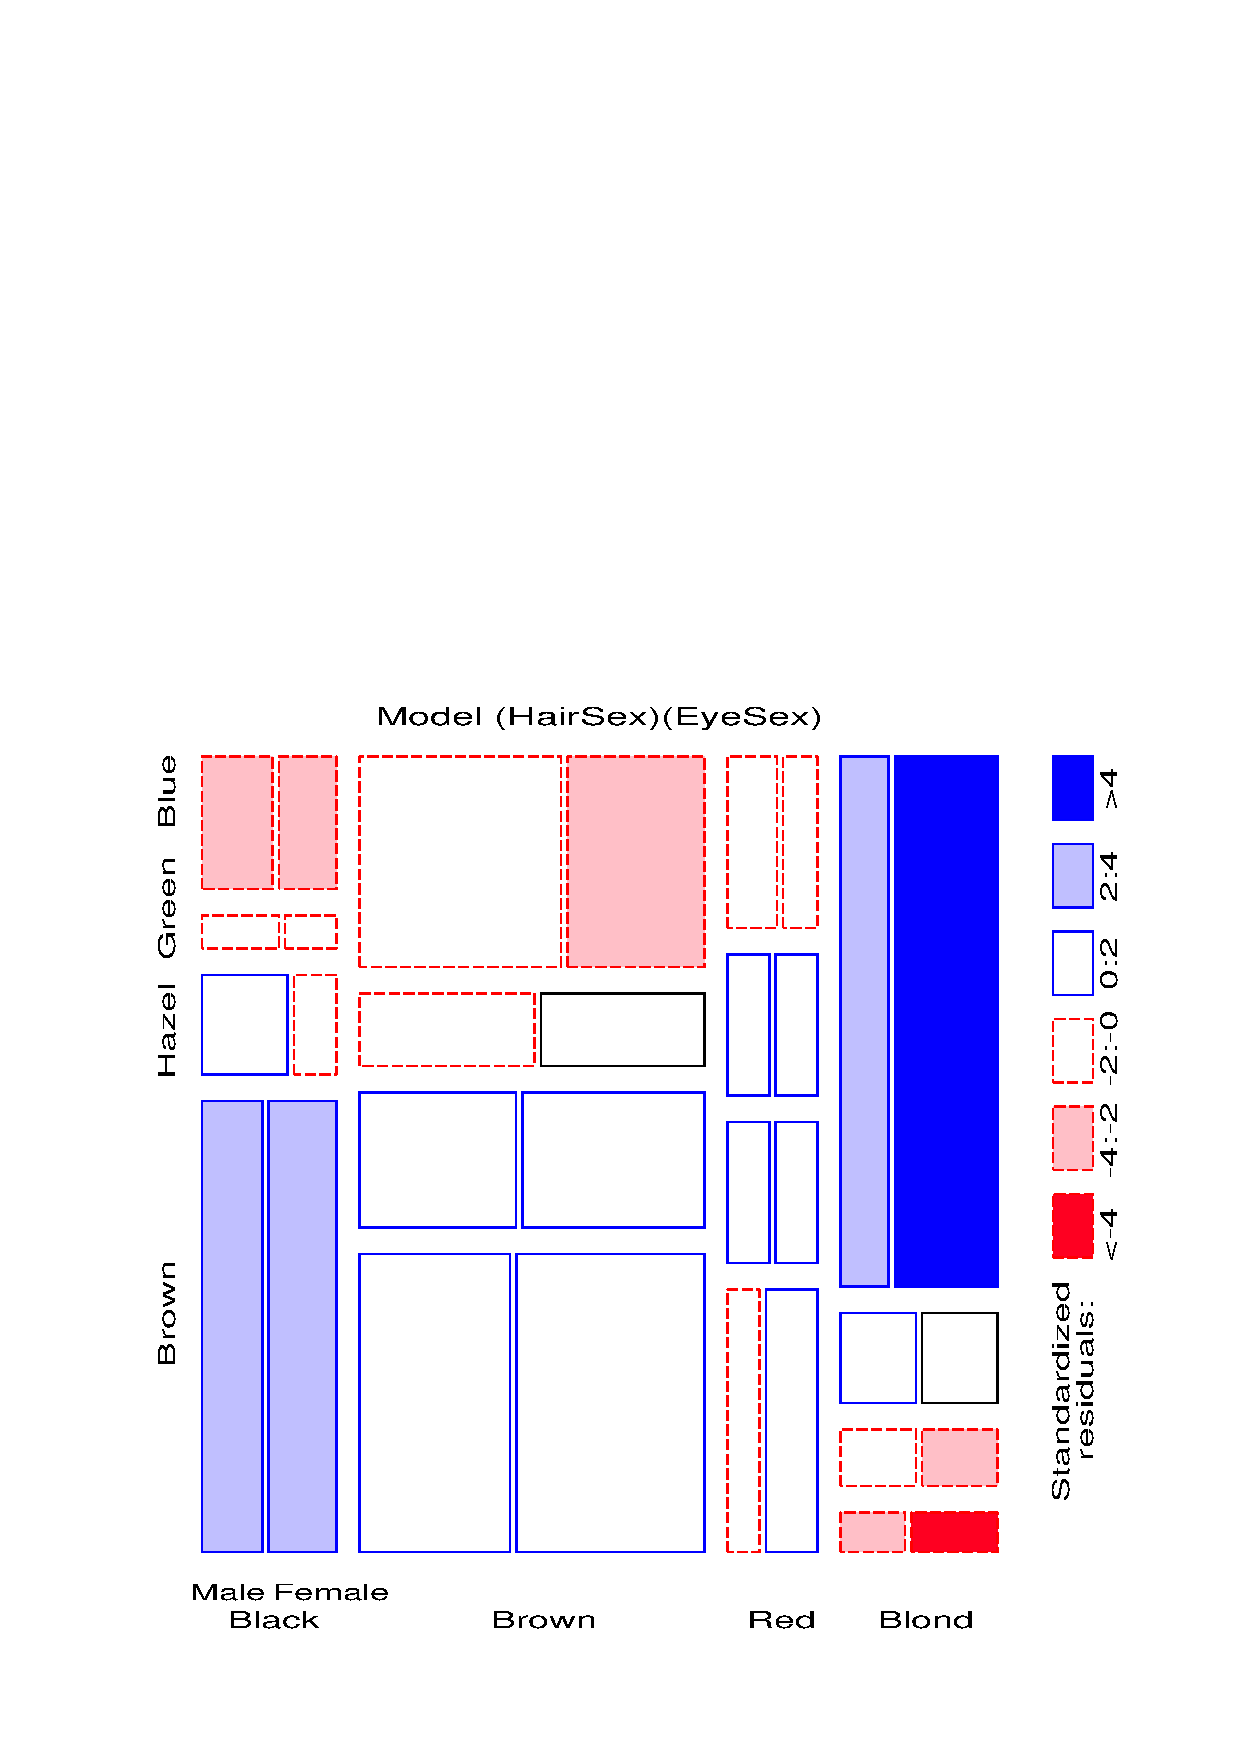
\includegraphics[scale=.6]{ch4/fig/mosaic36}
  \caption[Three-way mosaic, conditional independence]{Mosaic display for hair color, eye
color, and sex.  This display shows residuals from the model of
conditional independence, \([HS] \,  [ES] \), \(G^2\) = 156.68 on 18 df.}
  \label{fig:mosaic36}
\end{figure}

\subsubsection{Sequential plots and models}\label{sec:mosaic-seq}

The mosaic display is constructed in stages, with the variables
listed in a given order.
At each stage, the procedure
fits a (sub)model to the marginal subtable defined by summing over all
variables not yet entered.  For example for a three-way table,
$\{ABC\}$, the marginal subtables $\{A\}$ and $\{AB\}$ are calculated
in the process of constructing the three-way mosaic.
The $\{A\}$ marginal table can be fit to a model where the categories
of variable A are equiprobable (or some other discrete distribution);
the independence model can be fit to the $\{AB\}$ subtable, and so forth.

The series of plots can give greater insight into the relationships
among all the variables than a single plot alone.
Moreover, the series of mosaic plots fitting submodels of
joint independence to
the marginal subtables have the special property that they can be viewed as partitioning the hypothesis
of mutual independence in the full table.

For example, for the hair-eye data, the mosaic displays for the
\llmterm{Hair} \llmterm{Eye} marginal table (\figref{fig:mosaic34})
and the \llmterm{HairEye} \llmterm{Sex}
table (\figref{fig:mosaic35}) can be
viewed as representing the partition of $\GSQ$ shown below:
\begin{center}
\begin{tabular}{lrr}
Model               &    df    &  \(G^2\)  \\ \hline
\llmterm{Hair} \llmterm{Eye}        &     9    & 146.44 \\
\llmterm{Hair, Eye} \llmterm{Sex}   &    15    &  19.86 \\ \hline
\llmterm{Hair} \llmterm{Eye} \llmterm{Sex}  &    24    & 155.20
\end{tabular}
\end{center}

This partitioning scheme for sequential models of joint independence extends directly to higher-way tables.
The \sasprog{mosaics} implements a variety of schemes for fitting
a sequential series of submodels, including
mutual independence, joint independence, conditional independence,
partial independence and Markov chain models.

\subsubsection{Marginal Subtables and Simpson's Paradox}\label{sec:mosaic-marginal}

The sequential plots of marginal subtables assume that the (unconditional)
relationship among earlier variables in the ordering, ignoring later
variables, is the \emph{same}
as the (conditional) relationship among these variables controlling for
later ones.
For example, we assume that Hair color and Eye color have the same relation
in the marginal subtable as they do in the subtable for each sex separately.

It is possible, however, for the marginal relations among variables to
differ in magnitude, or even in direction, from the relations among
those variables controlling for additional variables.
The peculiar result that a pair of variables can have a marginal
association in a different direction than their partial associations
is called \glossterm{Simpson's paradox}.

One way to determine if the marginal relations are representative
is to fit models of conditional association
and compare them with the marginal models.
For the hair color, eye color data, the appropriate model is the model
\llmterm{Hair, Sex} \llmterm{Eye, Sex}, which
examines the relation between Hair color and Eye color controlling
for Sex.  The fit statistic is nearly the same as for the
unconditional marginal model:
\begin{center}
\begin{tabular}{lrr}
Model               &    df    &  \(G^2\)  \\ \hline
\llmterm{Hair} \llmterm{Eye}           &      9    & 146.44 \\
\llmterm{Hair, Sex} \llmterm{Eye, Sex} &     15    & 156.68 \\
\end{tabular}
\end{center}

And, the pattern of residuals is quite similar to that of the
\llmterm{Hair} \llmterm{Eye} marginal model, so we conclude there is no
such problem here.

In this section I have described a variety of models which can be fit
to higher-way tables, some relations among those models, and the aspects
of lack-of-fit which are revealed in the mosaic displays.
The following examples illustrate the process of model fitting,
using the mosaic as an interpretive guide to the nature of associations
among the variables.
In general, we start with a minimal baseline model.%
%
\footnote{When one variable, $R$
is a response, this normally is the model of joint independence,
\([E_1 E_2 \dots] \, [R]\), where \(E_1, E_2, \dots\) are the explanatory
variables.
}
The pattern of residuals in the mosaic will suggest associations to be added
to an adequate explanatory model.
As the model achieves better fit to the data, the degree of shading
decreases, so we may think of the process of model fitting as
``cleaning the mosaic.''


\subsection{Causal models}\label{sec:causal}

This sequence of models of joint independence has another
interpretation when the ordering of the variables is based on a set
of ordered hypotheses involving causal relationships among
variables 
(\citet{Goodman:73}, \citet[\S 7.2]{Fienberg:80}).  Suppose, for example,
that the causal ordering of four variables is \(A \rightarrow B
\rightarrow C \rightarrow D\), where the arrow means ``is antecedent
to.''  Goodman suggests that the conditional joint probabilities of
$B$, $C$, and $D$ given $A$ can be characterized by a set of
recursive logit models which treat
\begin{seriate}
\item $B$ as a response to $A$,
\item $C$
as a response to $A$ and $B$ jointly,
\item and $D$ as a response to $A$,
$B$ and $C$.
\end{seriate}
These are equivalent to the log-linear models which
we fit as the sequential baseline models of joint independence,
namely \LLM{A,B}, \LLM{AB,C}, and \LLM{ABC,D}.  The combination of these
models with the marginal probabilities of A gives a characterization
of the joint probabilities of all four variables.

\begin{Example}[marital1]{Marital status and pre- and extramarital sex}

A study of divorce patterns  by \citet{ThornesCollard:79} reported
the \(2^4\) table shown in  
\tabref{tab:maridat} (see \datref{dat:marital} for the SAS \Dset).
These data were analysed by \citet[\S 7.2.4]{Agresti:90}
and by \citet{Friendly:94a}, from which this account draws.
A sample of
about 500 people who had petitioned for divorce, and a similar number
of married people were asked two questions regarding their pre- and
extramarital sexual experience:  (1) ``Before you married your
(former) husband/wife, had you ever made love with anyone else?,''
(2) ``During your (former) marriage (did you) have you had any
affairs or brief sexual encounters with another man/woman?'' 
The
table variables are thus gender ($G$), reported premarital ($P$)
and extramarital ($E$) sex, and current marital status ($M$).


%%
%% Table marital written by md2tex 01MAY98 13:11
%%
\begin{table}[htb]
 \caption{Marital Status in Relation to Gender and Reported Premarital and Extramarital Sex}
 \label{tab:maridat}
 \begin{center}
  \begin{tabular}{|lll|rr|}
   \hline
{\bfseries\large Extramarital} & {\bfseries\large Premarital} &  & \multicolumn{2}{c|}{\bfseries\large Marital Status}\rule{0in}{2.5ex}\\
{\bfseries\large Sex} & {\bfseries\large Sex} & {\bfseries\large Gender} & Divorced  & Married   \\
   \hline
Yes            & Yes          & Women    &         17 &          4 \\
No             &              &          &         54 &         25 \\
[4pt]
Yes            & No           &          &         36 &          4 \\
No             &              &          &        214 &        322 \\
[4pt]
Yes            & Yes          & Men      &         28 &         11 \\
No             &              &          &         60 &         42 \\
[4pt]
Yes            & No           &          &         17 &          4 \\
No             &              &          &         68 &        130 \\
   \hline
\rule{0in}{2.5ex}{\bfseries\large Total} & & &       494 &        542 \\
   \hline
  \end{tabular}
 \end{center}
\end{table}


In this analysis we consider the variables in the order $G$, $P$,
$E$, and $M$.  That is, the first stage  treats $P$ as a
response to $G$ and examines the [Gender][Pre] mosaic to assess
whether gender has an effect on premarital sex.  The second stage
treats $E$ as a response to $G$ and $P$ jointly;  the
mosaic for [Gender, Pre] [Extra] shows whether extramarital sex
is related to either gender or premarital sex.  Finally, the mosaic
for [Gender, Pre, Extra] [Marital] is examined for evidence of the
dependence of marital status on the three previous variables jointly.
As noted above, these models are equivalent to the
recursive logit models whose path diagram is \(G \rightarrow P
\rightarrow E \rightarrow M\).%
\footnote{ \citet[\S 7.2.4]{Agresti:90} considers a slightly more complex,
but more realistic model in which premarital sex affects both the propensity
to have extramarital sex and subsequent marital status.}
The \(G^2\) values for these models
shown below provide a decomposition of the
\(G^2\) for the model of complete independence fit to the full table.

\begin{center}
 \begin{tabular}{rrr}
 \hline
  Model        & df & \(G^2\) \\ 
 \hline
  \llmtwo{G}{P}    & 1  & 75.259 \\ 
  \llmtwo{GP}{E}   & 3  & 48.929 \\ 
  \llmtwo{GPE}{M}  & 7  & 107.956 \\ 
 \hline
  \llmfour{G}{P}{E}{M} & 11 & 232.142 \\ 
 \hline
 \end{tabular}
\end{center}

The [Gender] [Pre] mosaic is shown in \figref{fig:mosaic51}.
The mosaic shows that men are much more likely to report
premarital sex than are women; the sample odds ratio is 3.7.  We
also see that women are about twice as prevalent as men in this
sample.

%% two figures side-by-side
\begin{figure}[htb]
 \begin{minipage}[b]{.49\linewidth}
  \centering
  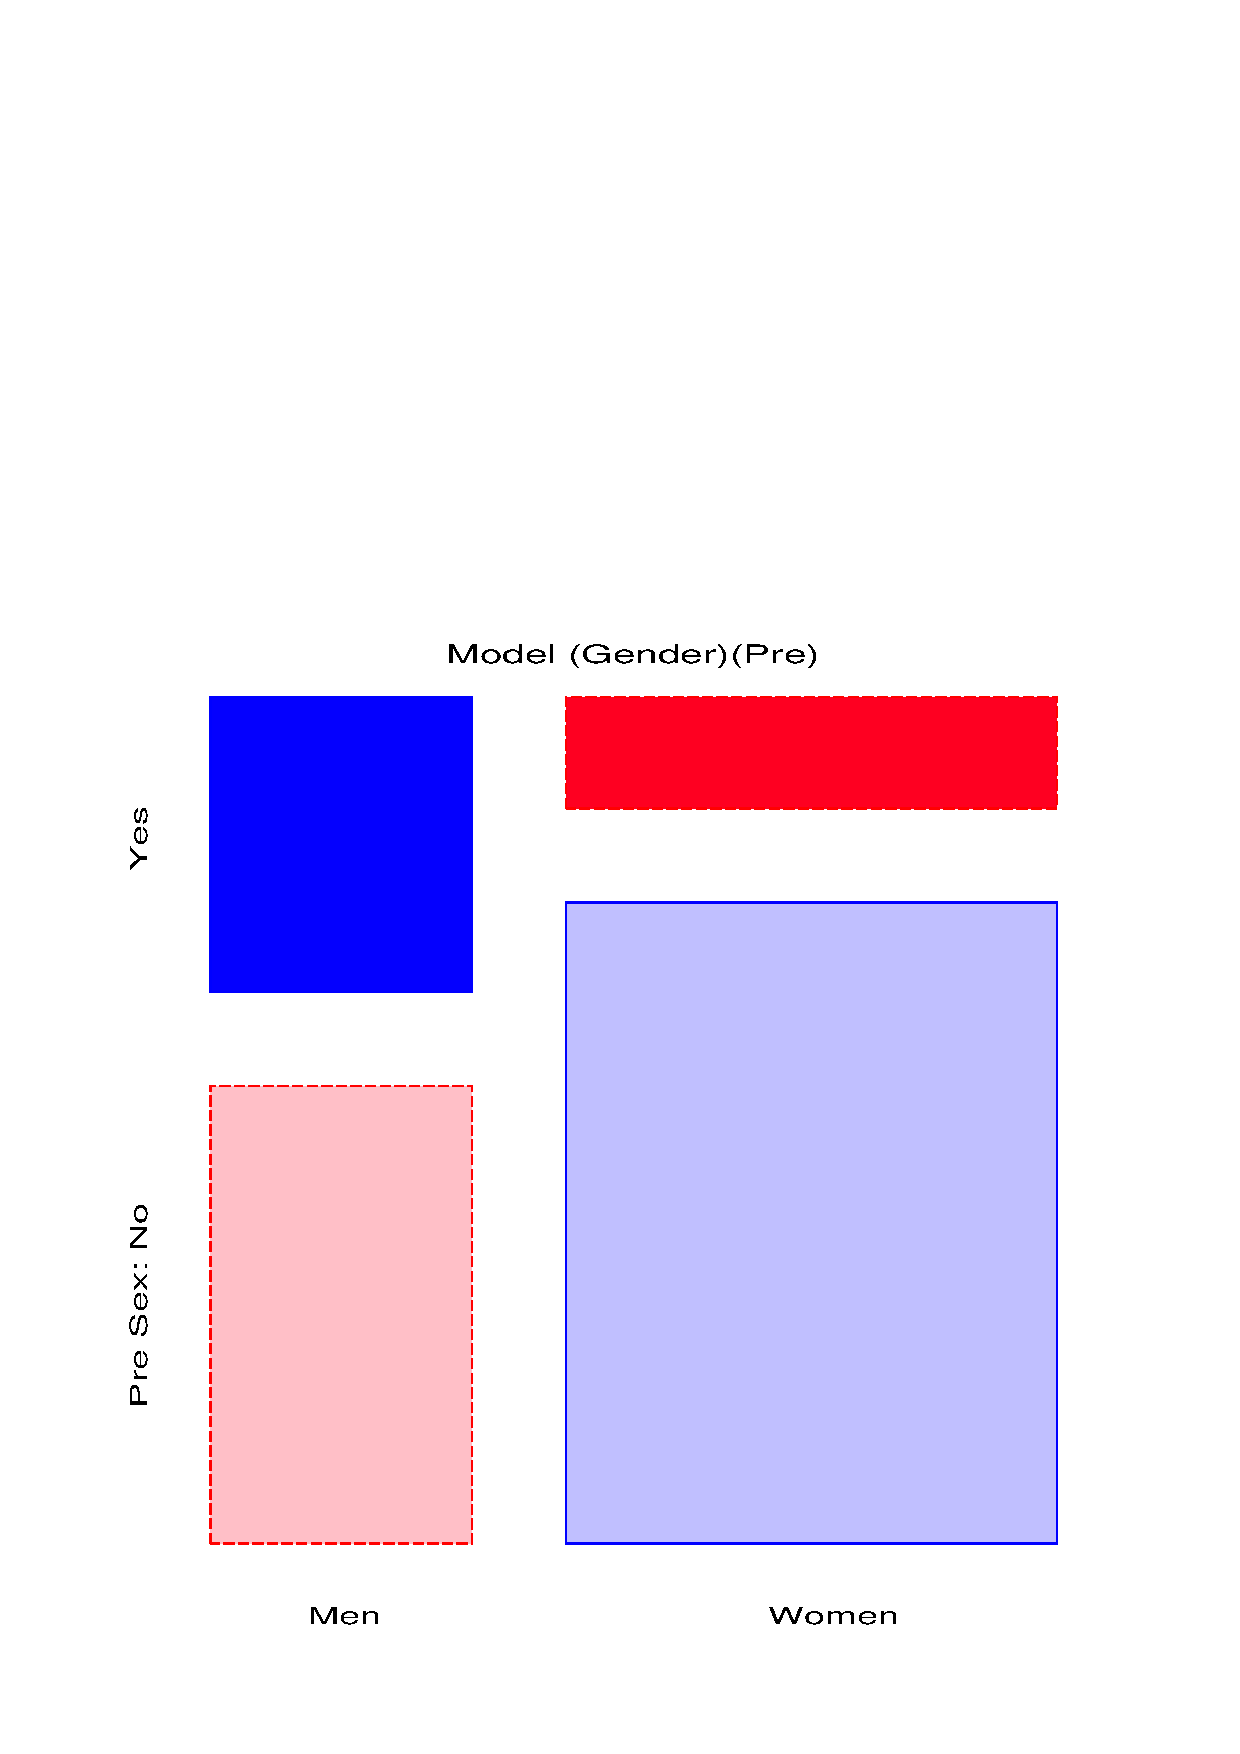
\includegraphics[width=1\linewidth]{ch4/fig/mosaic51}
  \caption[Mosaic display for gender and
pre-martial sexual experience]{Mosaic display for gender and
pre-martial sexual experience.}%
  \label{fig:mosaic51}
 \end{minipage}%
 \hfill
 \begin{minipage}[b]{.49\linewidth}
  \centering
  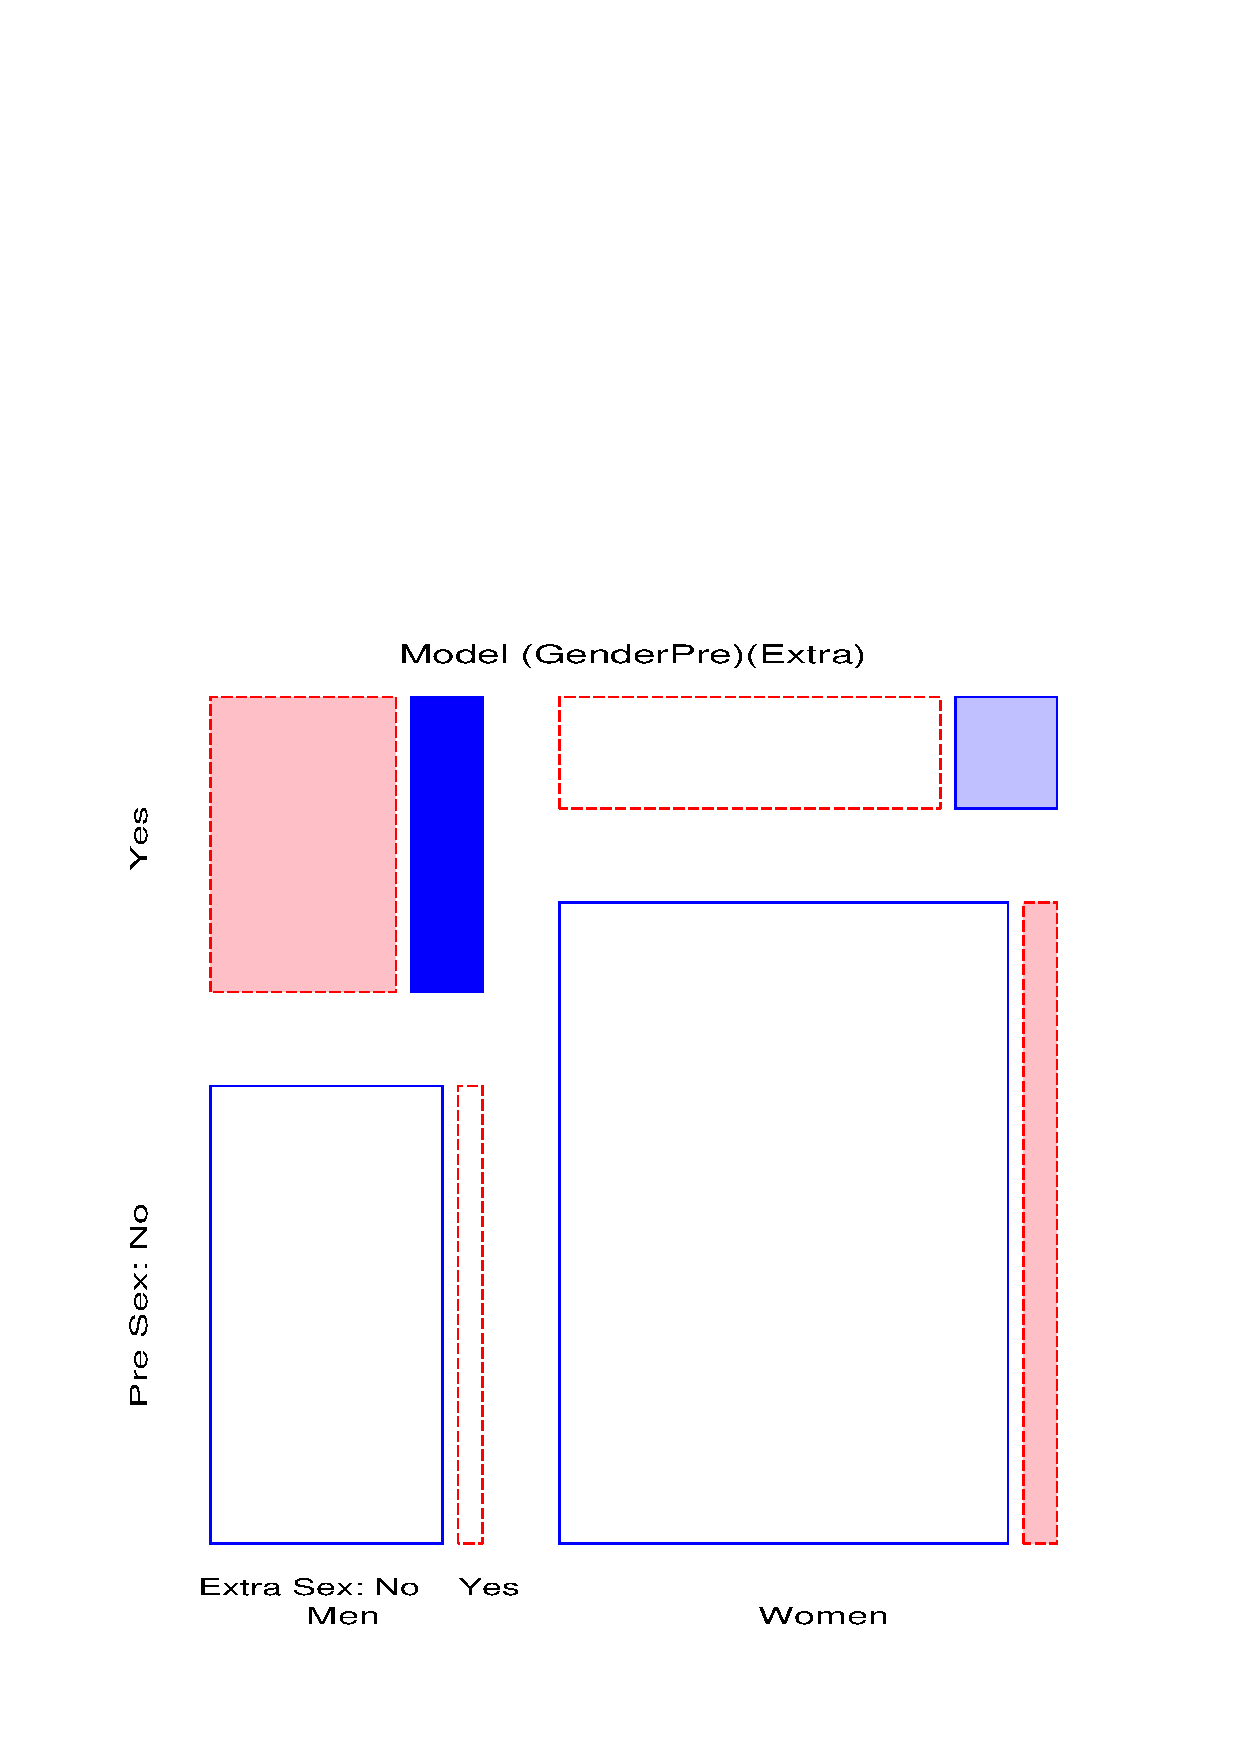
\includegraphics[width=1\linewidth]{ch4/fig/mosaic52}
  \caption[Mosaic display for the model of
joint independence]{Mosaic display for the model of
joint independence, \llmtwo{GP}{E}.}\label{fig:mosaic52}
 \end{minipage}
\end{figure}

For the second stage, the [Gender, Pre][Extra] mosaic is shown in 
\figref{fig:mosaic52}.  \GSQ\ for the model \LLM{GP,E}
is 48.93 on 3 \(df\), indicating that extramarital sex
depends on
gender and premarital sex jointly.  From the pattern
of residuals in \figref{fig:mosaic52} we see that men and
women who have reported premarital sex are far more likely to report
extramarital sex than those who have not.  From the marginal totals
for the [GP] [E] table, the conditional odds ratio of extramarital
sex is 3.61 for men and 3.56 for women.  Thus, extramarital sex
depends on premarital sex, but not on gender.


\figref{fig:mosaic53} shows the mosaic for the final stage, fitting
the model [Gender, Pre, Extra] [Marital].
It shows that
marital status depends
strongly on gender, premarital sex, and extramarital sex jointly.
Among those reporting no
premarital sex (bottom part of \figref{fig:mosaic53}), there
is a similar pattern of cell sizes and deviations for marital status
in relation to gender and extramarital sex:  People who did
not report premarital sexual experience are more likely to
remain married if they report no extramarital sex and more likely
to be divorced if they did.  Among those who do report premarital
sex (top part of \figref{fig:mosaic53}), there is also a similar
pattern of sign of deviations, positive for those who are divorced,
negative for those who are married.

%% two figures side-by-side
\begin{figure}[htb]
 \begin{minipage}[t]{.49\linewidth}
  \centering
  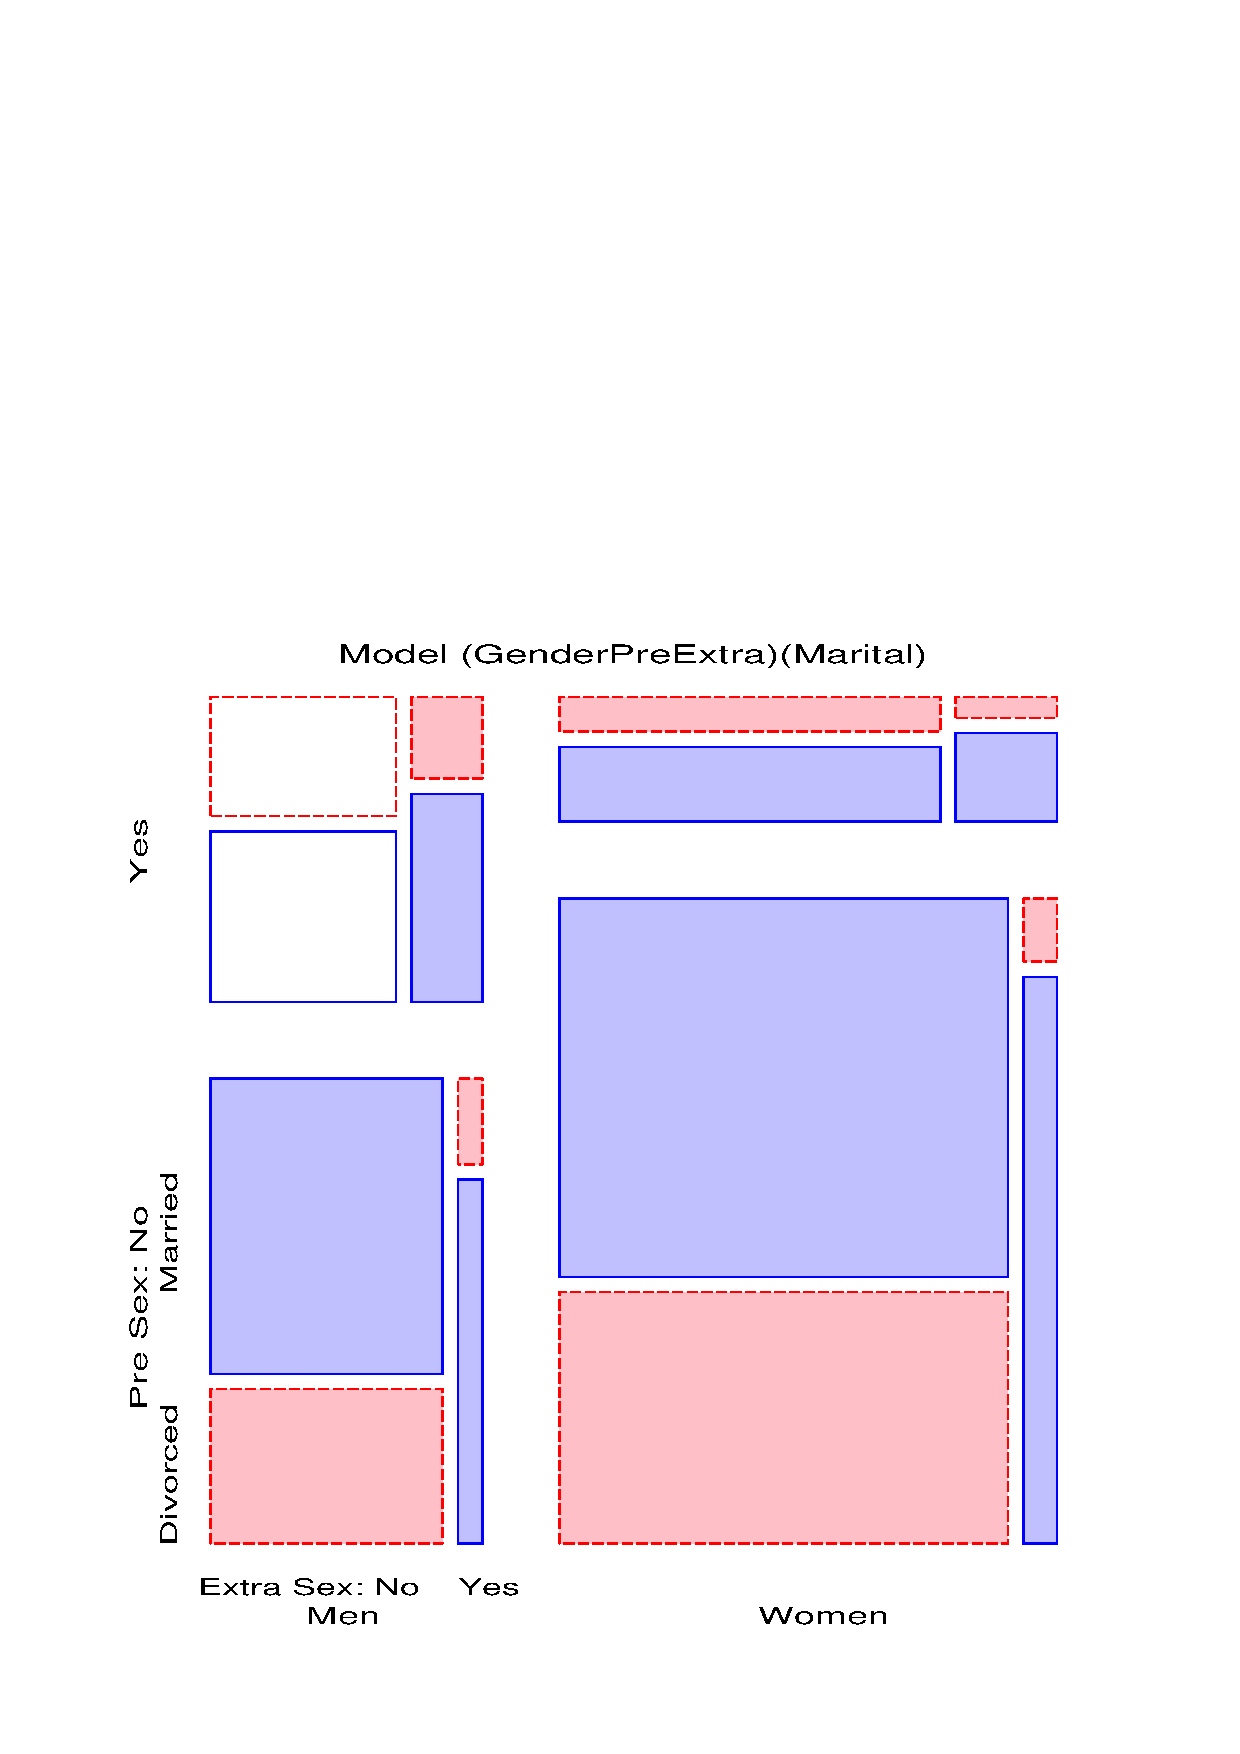
\includegraphics[width=1\linewidth]{ch4/fig/mosaic53}
  \caption[Four-way mosaic for the model \llmterm{GPE} \llmterm{M}]{Four-way mosaic for the model \llmterm{GPE} \llmterm{M}.  The pattern of residuals suggests terms to be included
in an explanatory model.}%
  \label{fig:mosaic53}
 \end{minipage}%
 \hfill
 \begin{minipage}[t]{.49\linewidth}
  \centering
  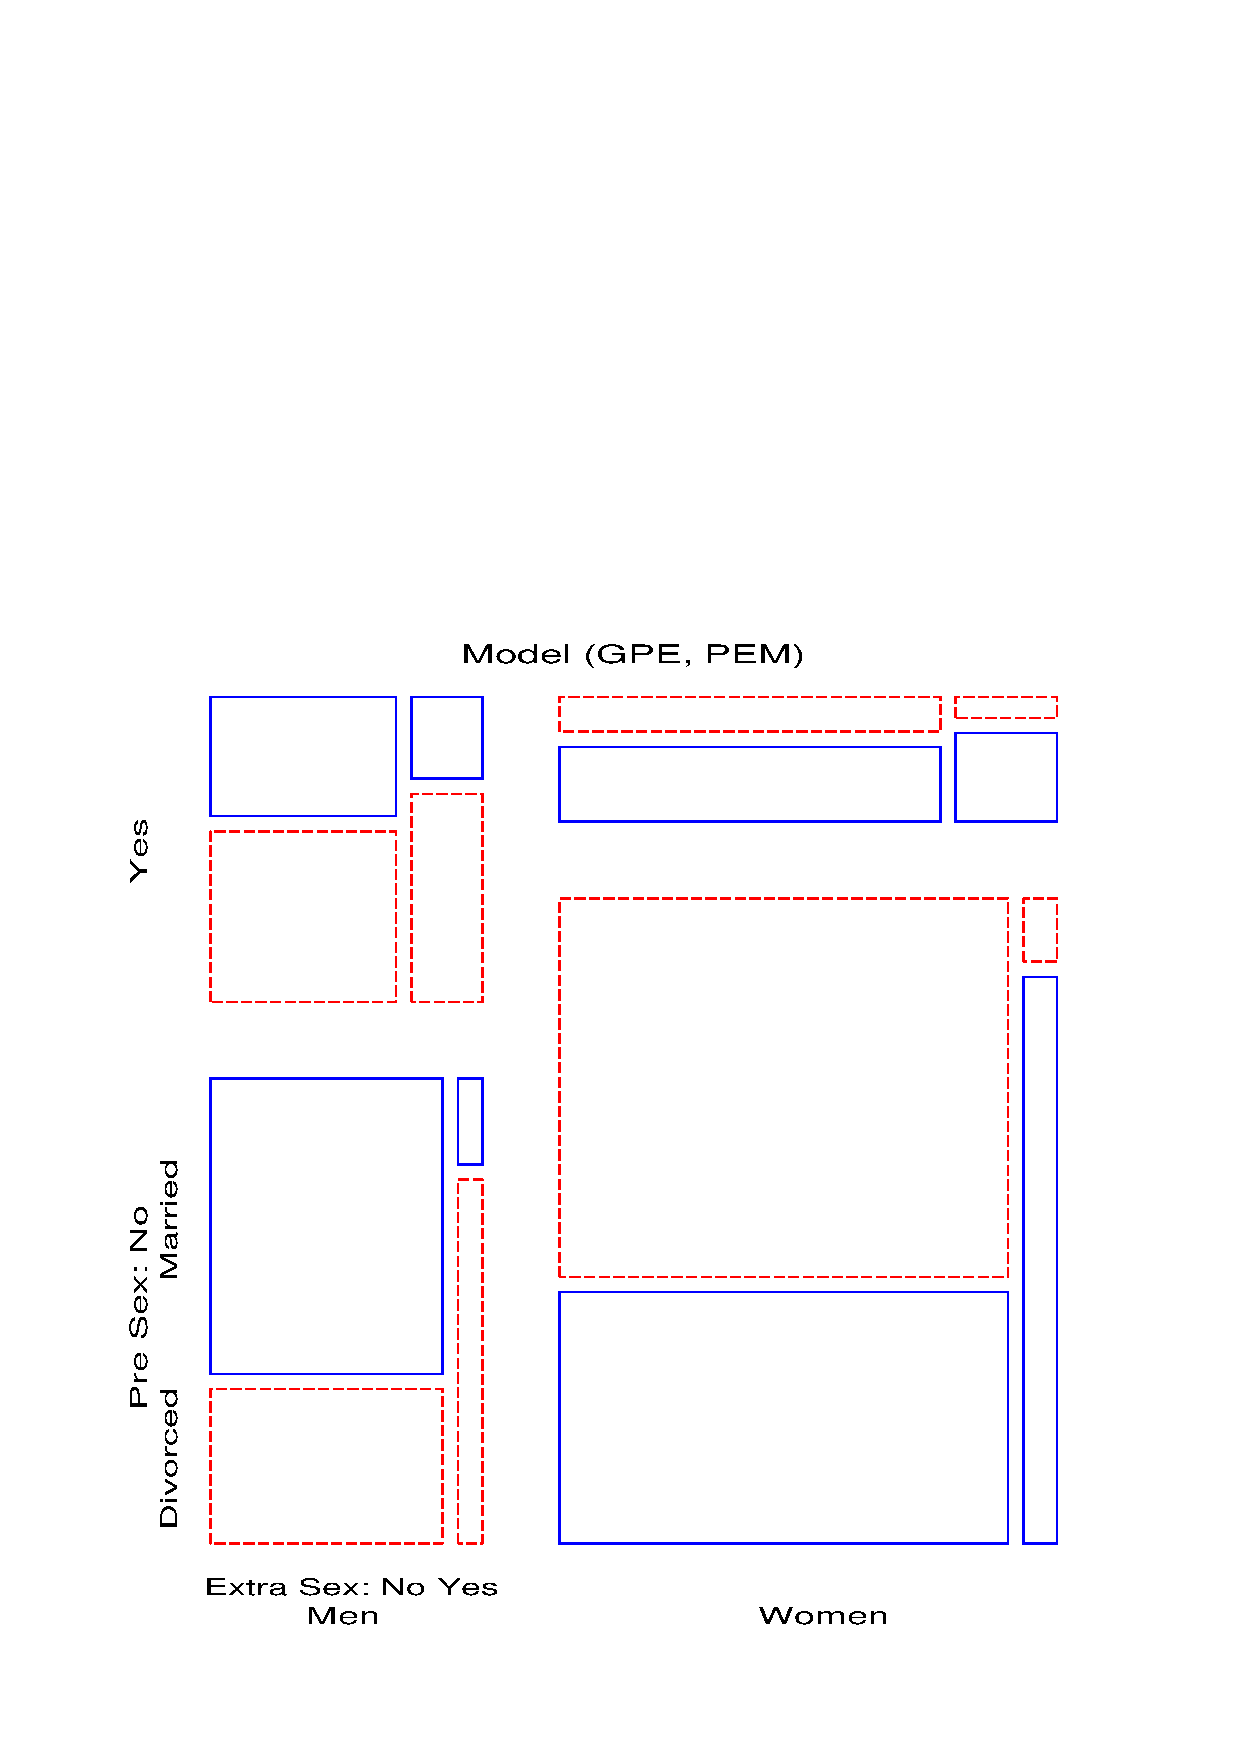
\includegraphics[width=1\linewidth]{ch4/fig/mosaic54}
  \caption[Four-way mosaic for the model \llmterm{GPE} \llmterm{PEM}]{Four-way mosaic for the model \llmterm{GPE} \llmterm{PEM}.} \label{fig:mosaic54}
 \end{minipage}
\end{figure}

The four \(2 \times  2\) blocks in \figref{fig:mosaic53} show the conditional
relation of extramarital sex to marital status.  Comparing these, we
see that the odds ratios of divorce in relation to reported
extra-martial sex are considerably larger for men and women who also
reported premarital sex.  These observations imply the need to
incorporate associations \llmterm{PM} and \llmterm{EM} of premarital and
extramarital sex with marital status, and probably the three-way association
\llmterm{PEM} into an explanatory model.
Since this stage
considers marital status as a response to gender, premarital sex and
extramarital sex, we would normally fit the $\{GPE\}$ marginal
table exactly, and consider the models \LLM{GEP,PM,EM} or 
\LLM{GPE,PEM} for the complete table.

The model \LLM{GPE,PM,EM} does not fit particularly well
(this mosaic is not shown here),
producing \(G^2  =  18.16\) on 5 \(df\) \(( p  =  .0028 )\).
The model \LLM{GPE,PEM}, however, does  fit quite well, \(G^2  =  5.25\)
with 4 \(df\) \(( p  =  .26 )\).
The term \llmterm{PEM} indicates that premarital sex and extramarital
sex interact in their effects on marital status:
The effect of extramarital sex on divorce is much greater for those
who had no premarital sex than for those who did!
The final mosaic for this model, shown in \figref{fig:mosaic54},
still shows some slight structure in the pattern of signs
of residuals (compare the blocks for men with those for women),
but all residuals are quite small.
\end{Example}
\begin{Example}[titanic]{Survival on the \emph{Titanic}}
There have been few marine disasters resulting in the staggering loss of life
than that
which occurred in the sinking of the \emph{Titanic} on April 15, 1912
and (perhaps as a result) few that are so widely known by the public.
It is surprising, therefore, that
neither the exact death toll from this disaster
nor the distributions of death among the passengers
and crew are widely agreed.
\citet[Table 2]{Dawson:95} presents the cross-classification of
2201 passengers and crew on the \emph{Titanic} by Age, Gender, Class
(1st, 2nd, 3rd, Crew) shown in \tabref{tab:titanic} 
(see also \datref{dat:titanic})
and describes his efforts to reconcile various historical sources.
Let us see what we can learn from this \Dset.

%%
%% Table titanic written by md2tex 09APR99 14:57
%%
\begin{table}[htb]
 \caption{Survival on the Titanic}
 \label{tab:titanic}
 \begin{center}
  \begin{tabular}{|lll|rrrr|}
   \hline
 &  &  & \multicolumn{4}{c|}{\bfseries\large Class   }\rule{0in}{2.5ex}\\
{\bfseries\large Gender     } & {\bfseries\large Age     } & {\bfseries\large Survived} & 1st      & 2nd      & 3rd      & Crew     \\
   \hline
Male     & Adult   & Died       &    118 &    154 &    387 &    670 \\
Female   &         &            &      4 &     13 &     89 &      3 \\
[4pt]
Male     & Child   &            &      0 &      0 &     35 &      0 \\
Female   &         &            &      0 &      0 &     17 &      0 \\
[4pt]
Male     & Adult   & Survived   &     57 &     14 &     75 &    192 \\
Female   &         &            &    140 &     80 &     76 &     20 \\
[4pt]
Male     & Child   &            &      5 &     11 &     13 &      0 \\
Female   &         &            &      1 &     13 &     14 &      0 \\
   \hline
  \end{tabular}
 \end{center}
\end{table}


Examining the series of mosaics for the variables ordered
Class, Gender, Age, Survival will show the relationships among
the background variables and how these are related to survival.
The letters $C, G, A, S$ respectively are used to refer to these variables
below.

\figref{fig:mostitanic1} and \figref{fig:mostitanic2}
show the two-way and three-way plots among the background variables.
\figref{fig:mostitanic1} shows that the proportion of males decreases
with increasing economic class, and that the crew was almost entirely male.
The three-way plot (\figref{fig:mostitanic2})
shows the distribution of adults and children among the Class-Gender groups. The
residuals display the fit of a model in which Age is jointly independent of
the Class-Gender categories.
Note that there were no children among the crew, and the overall
proportion of children was quite small (about 5 \%).
Among the passengers, the proportion of children is smallest in
first class, largest in third class.
The only large positive residuals correspond to a greater number of children
among the 3rd class passengers, perhaps representing families traveling
or immigrating together.
%
% subfigmatrix 2 x 1
\begin{figure}[htb]
 \begin{subfigmatrix}{2}
 \subfigure[Class and Gender]{\label{fig:mostitanic1}%
  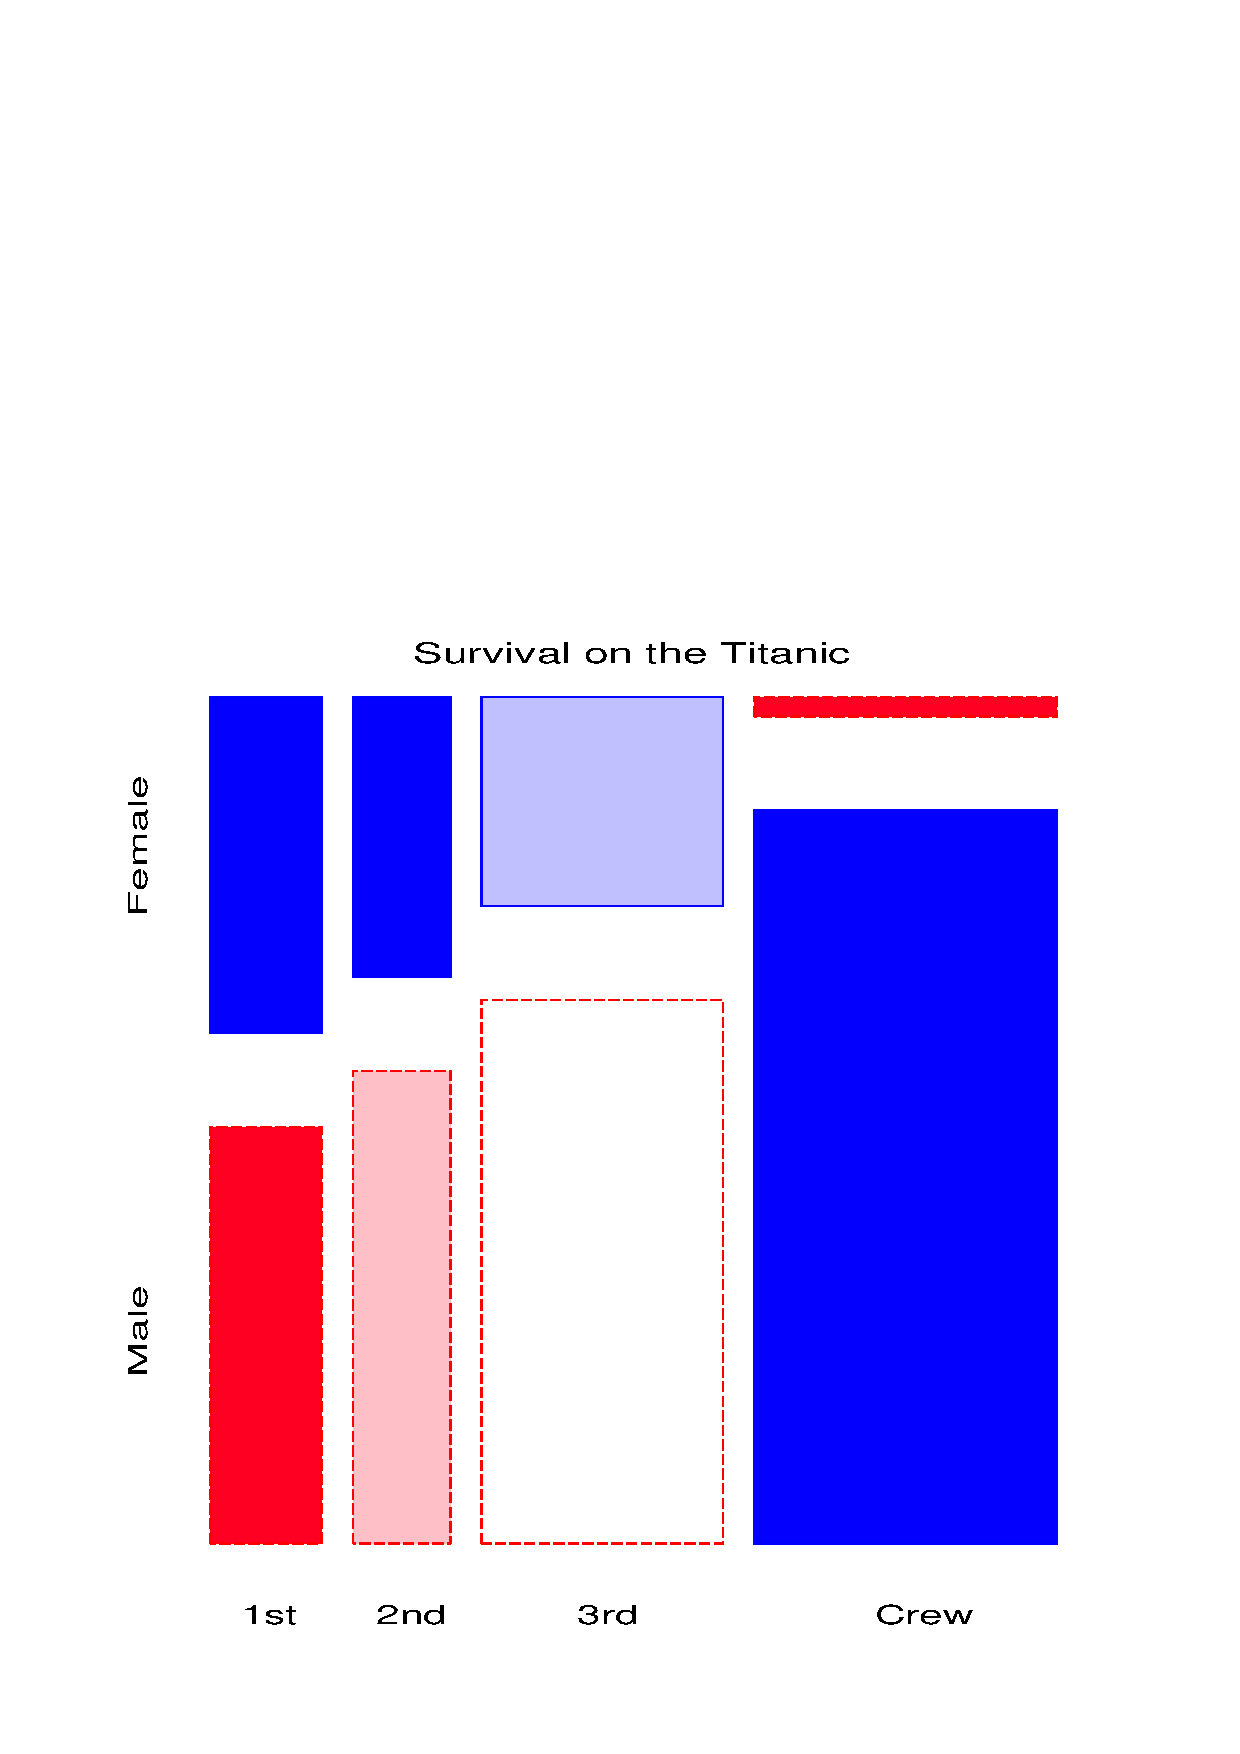
\includegraphics{ch4/fig/mostitanic1}
 }
 \subfigure[Class, Gender, Age]{\label{fig:mostitanic2}%
  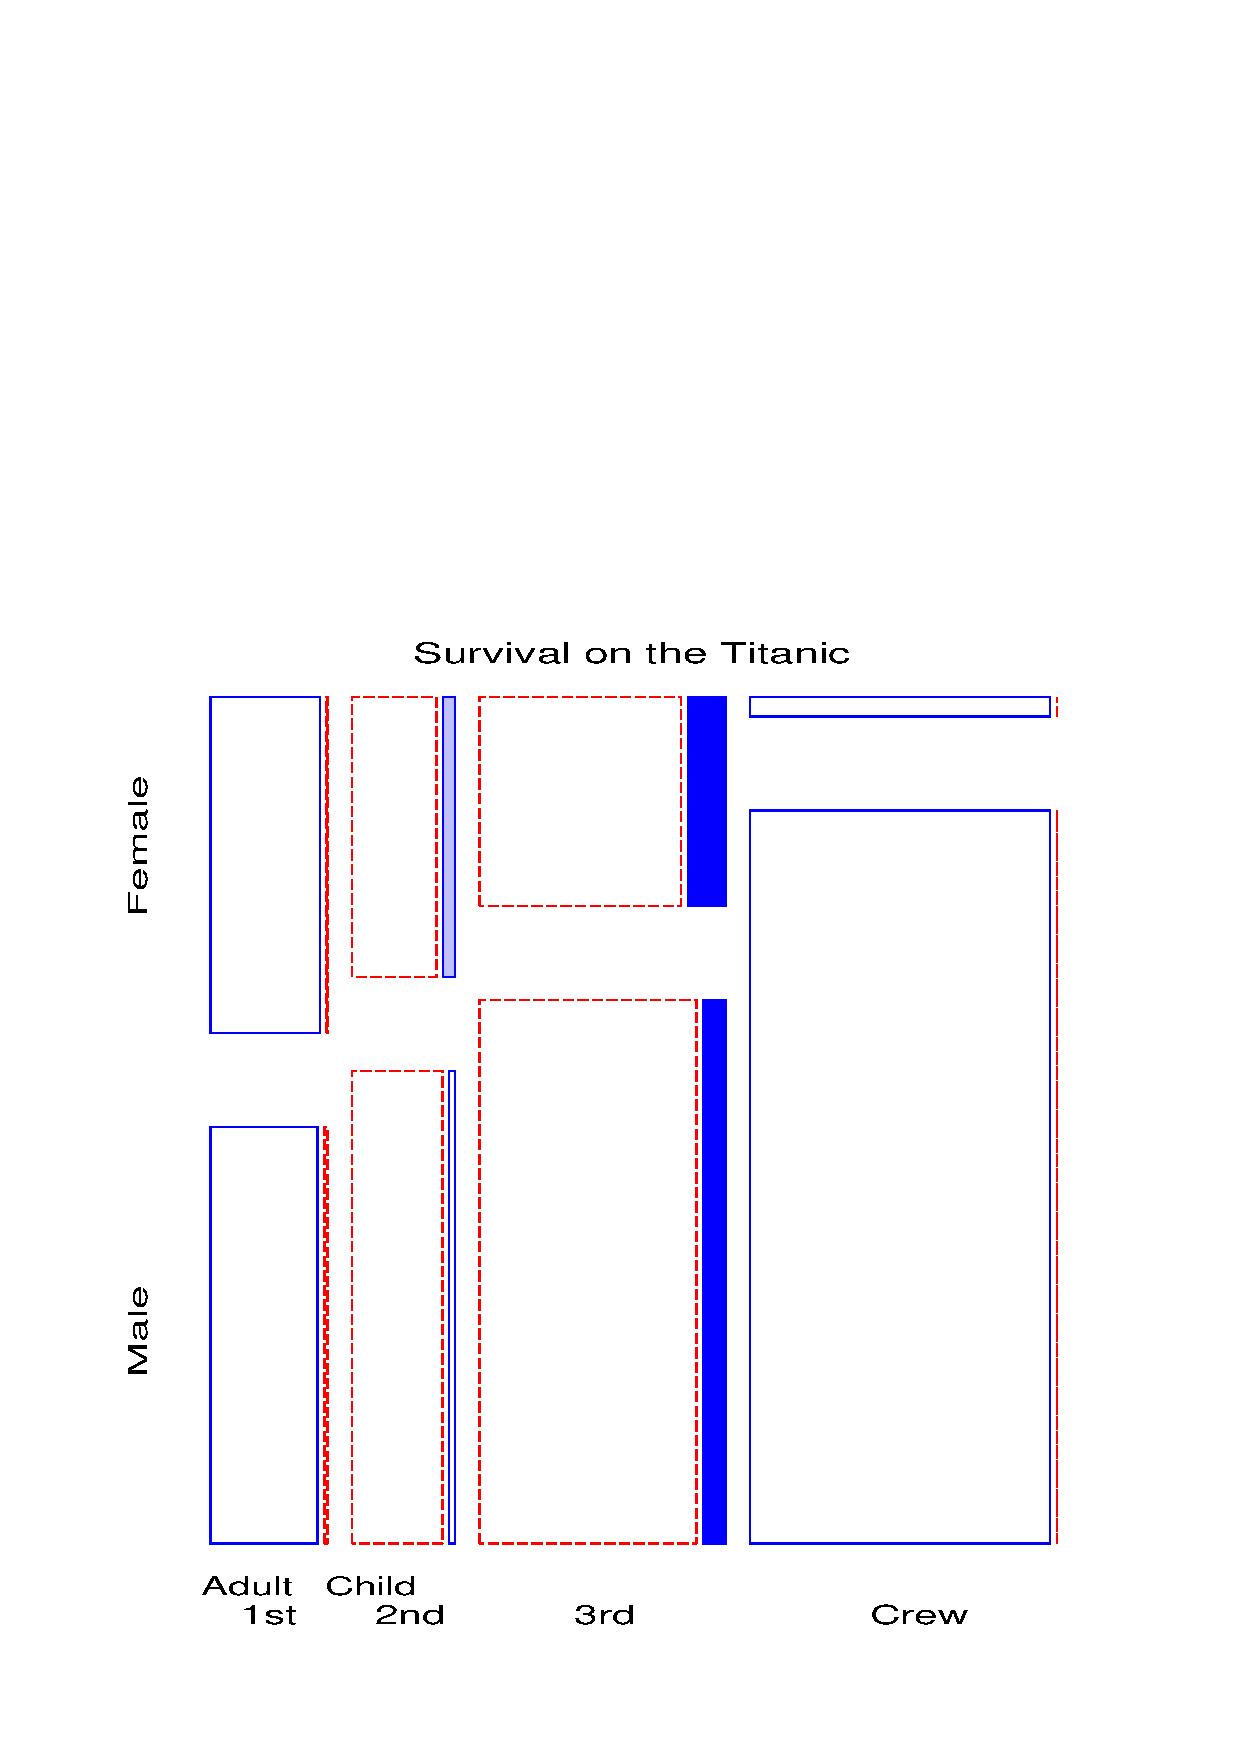
\includegraphics{ch4/fig/mostitanic2}
 }
 \end{subfigmatrix}
 \caption[Titanic data: Background variables]{Titanic data: Background variables}\label{fig:mostitanic1-2}
\end{figure}


The four-way mosaic, shown in \figref{fig:mostitanic3},
fits the model $[CGA][S]$ which asserts that survival is independent
of Class, Gender and Age.
This is the minimal null model when the first three variables are
explanatory.  It is clear that greater proportions of women survived
than men in all classes, but with greater proportions of women surviving
in the upper two classes.  Among males the proportion who survived
also increases with economic class (towards 1st class).
However, this model fits very poorly
($G^2 (15) = 671.96$),
and we may try to fit a more adequate model by adding associations between
survival and the explanatory variables.

Adding an association of each of Class, Gender and Age with Survival
amounts to fitting the model
\LLM{CGA,CS,GS,AS}.  That is, each of the three variables is
associated with survival, but have independent, additive effects. The mosaic for this model is shown in \figref{fig:mostitanic4}.
The fit of this model is much improved ($\Delta G^2 (5) = 559.4$), but still does not represent
an adequate fit ($G^2 (10) = 112.56$).
There are obviously interactions among Class, Gender and Age on their
impact on survival, some of which we have already noted.
%
% subfigmatrix 2 x 1
\begin{figure}[htb]
 \begin{subfigmatrix}{2}
 \subfigure[Joint independence: \LLM{CGA,S}]{\label{fig:mostitanic3}%
  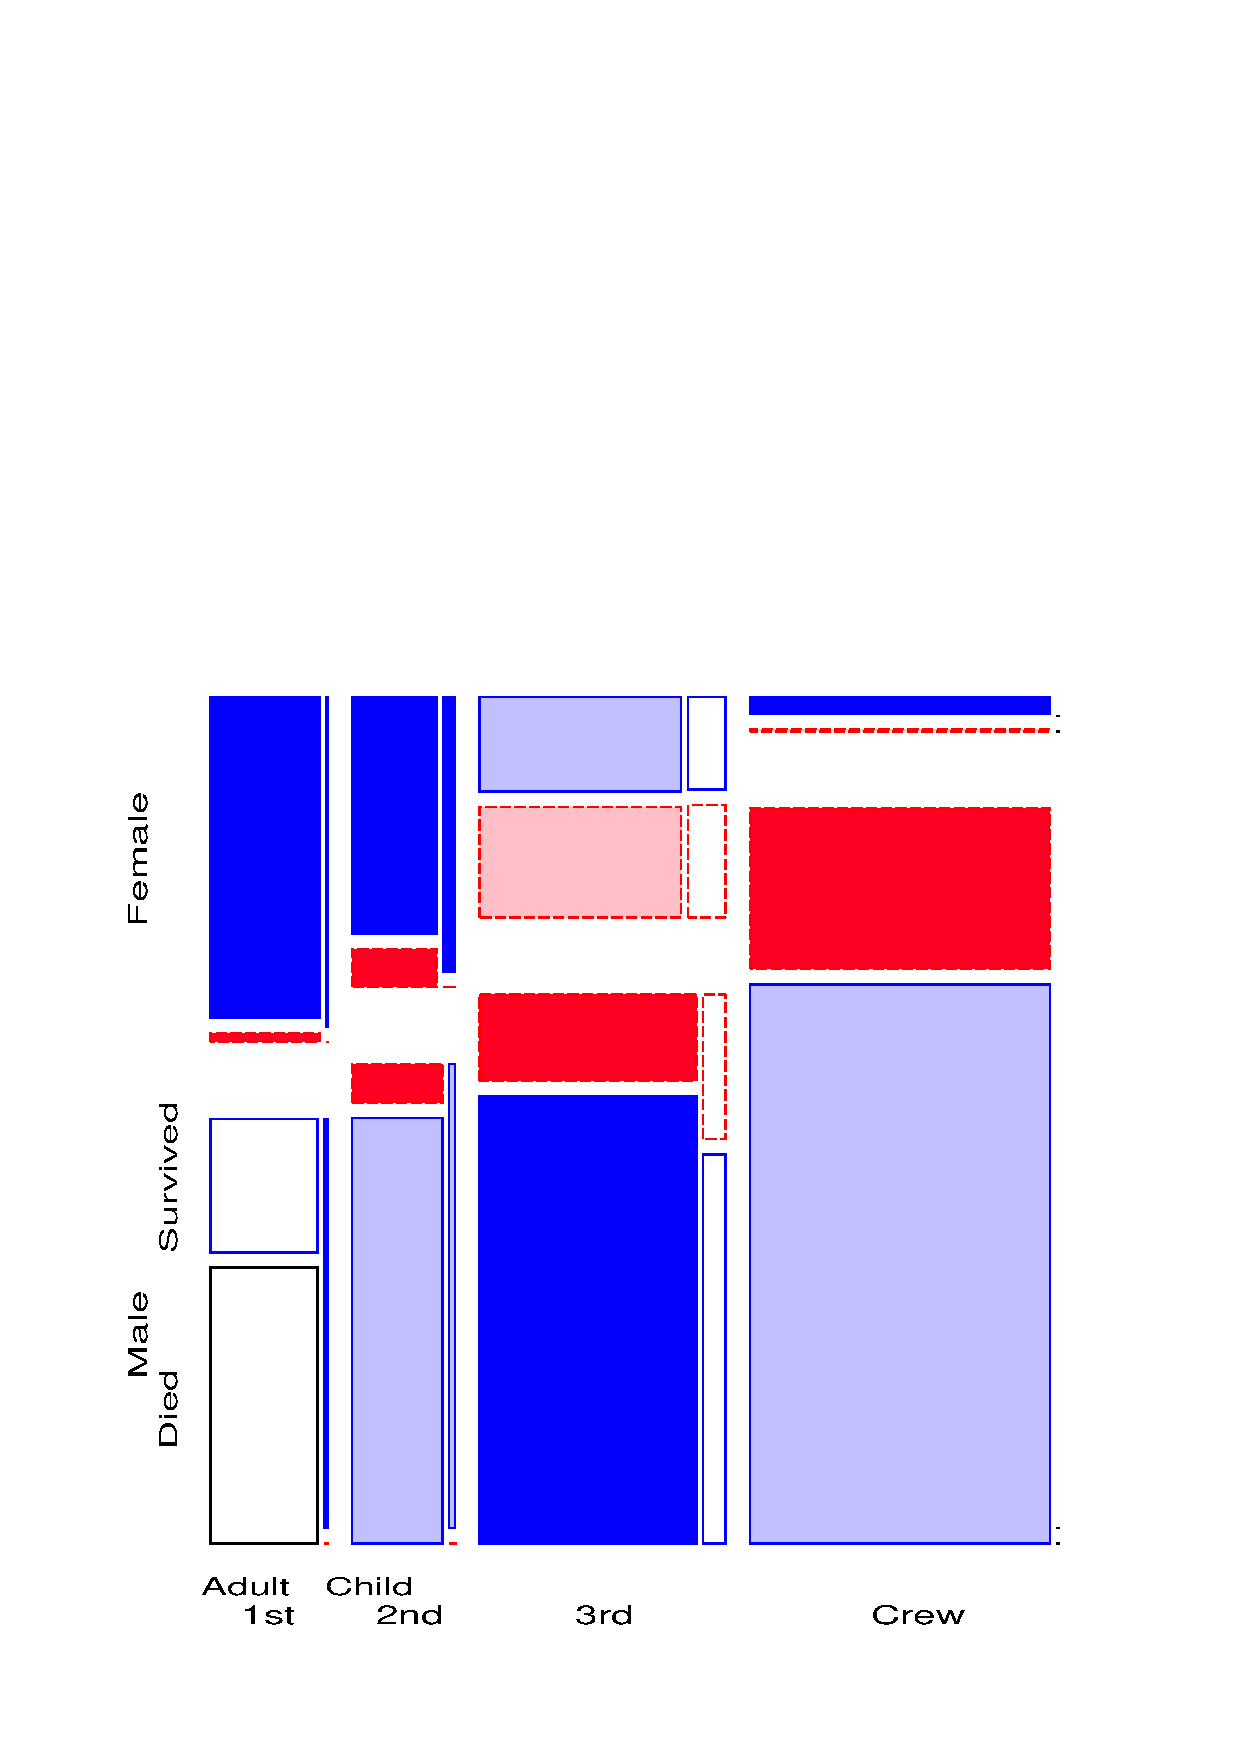
\includegraphics{ch4/fig/mostitanic3}
 }
 \subfigure[Effects of Age, Gender and Class on Survival: \LLM{CGA,CS,GS,AS}]{\label{fig:mostitanic4}%
  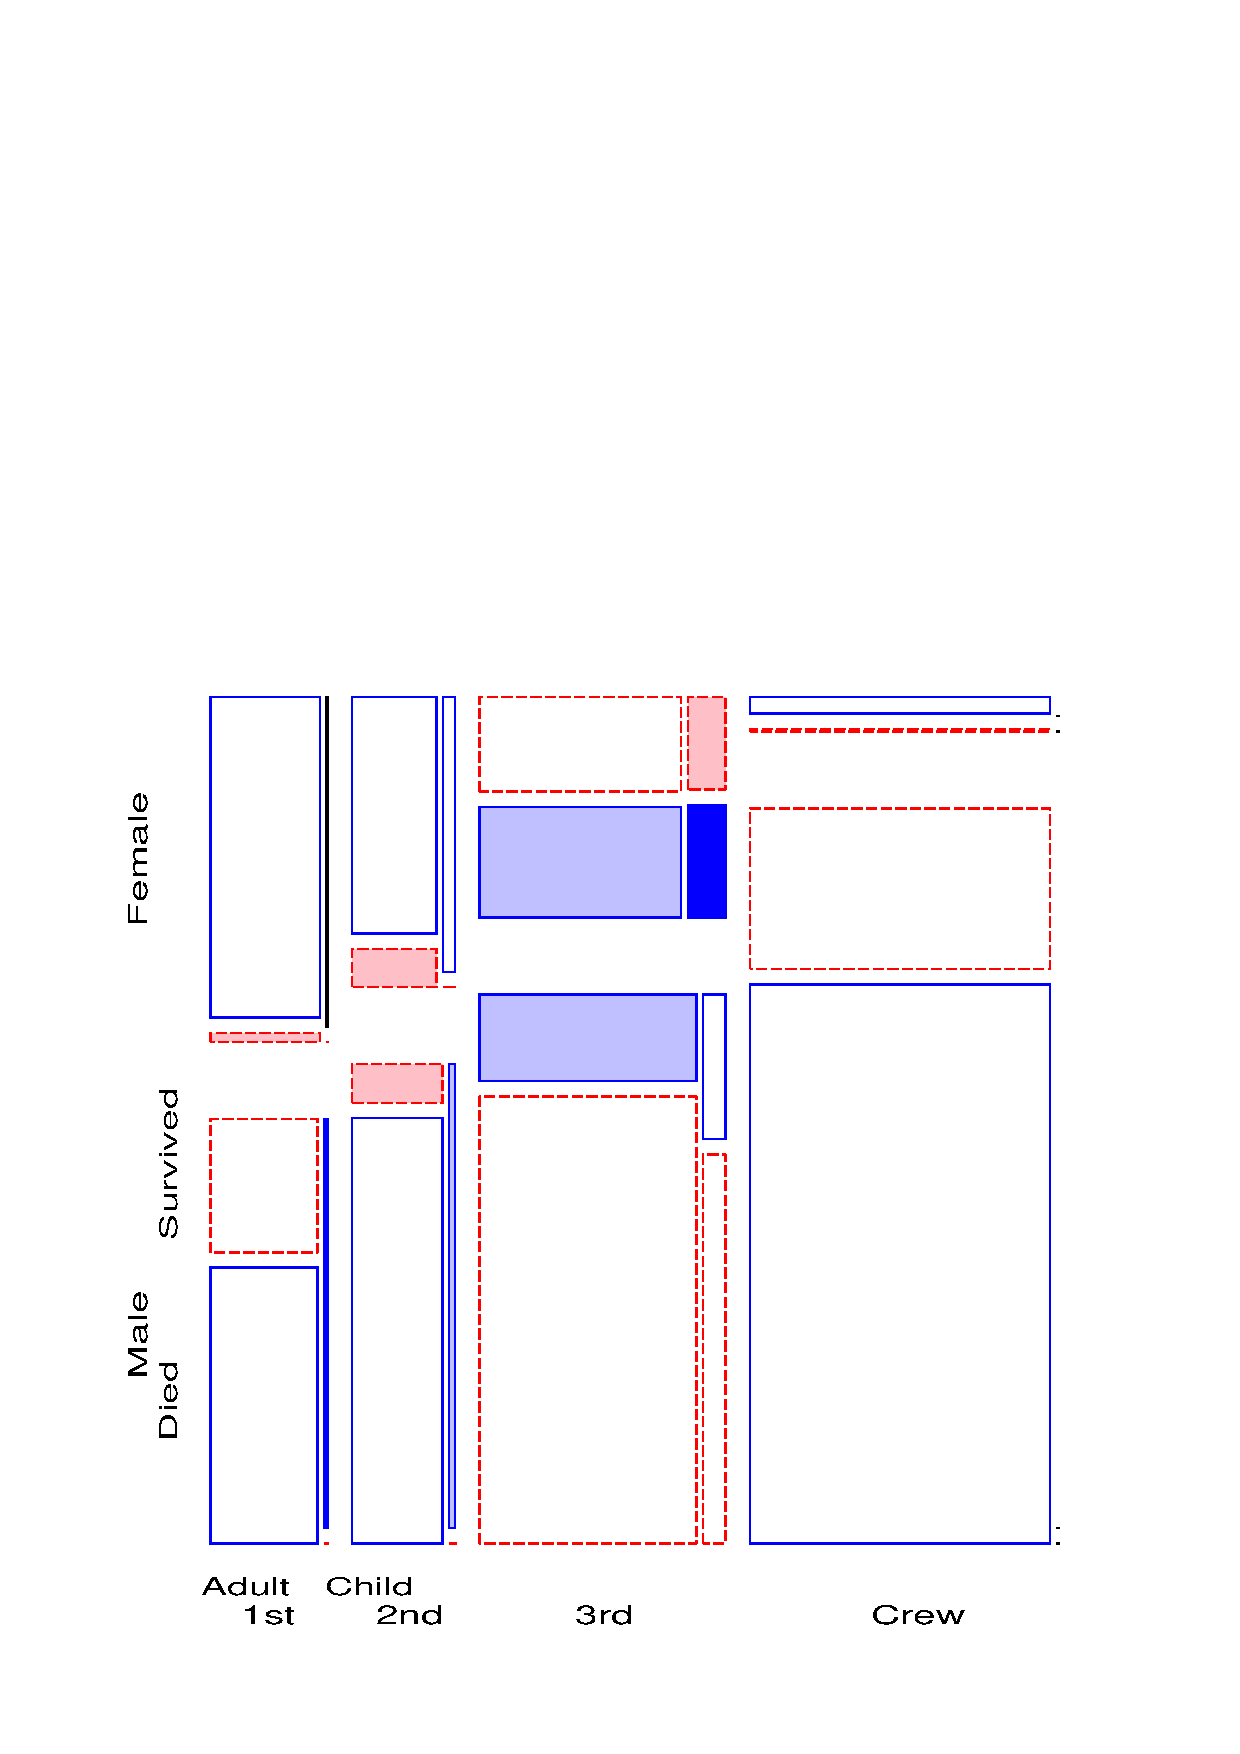
\includegraphics{ch4/fig/mostitanic4}
 }
 \end{subfigmatrix}
 \caption[Titanic data: Class, Gender, Age, and Survival]{Titanic data: Class, Gender, Age, and Survival}\label{fig:mostitanic3-4}
\end{figure}
%

Taking the rubric of ``women and children first,'' we next fit the
model \LLM{CGA,CS,GAS} in which Age and Gender interact in their influence
on survival.  The mosaic for this model is shown in \figref{fig:mostitanic5}.
Adding the association of Age and Gender with survival has
improved the model slightly, however the fit is still not good ($G^2 (9) = 94.54$).
If we add the interaction of Class and Gender to this
(the model \LLM{CGA,CGS,GAS}) the \LR{} chi-square is reduced
substantially ($G^2 (6) = 37.26$), but the lack of fit is still
significant.

Finally, we try a model in which Class interacts with both
Age and Gender to give the model
\LLM{CGA,CGS,CAS}, whose residuals are shown in \figref{fig:mostitanic6}.
The \LR{} chi-square is now 1.69 with 4 df, a very good fit, indeed.
%
% subfigmatrix 2 x 1
\begin{figure}[htb]
 \begin{subfigmatrix}{2}
 \subfigure[Model \LLM{CGA,CS,GAS}]{\label{fig:mostitanic5}%
  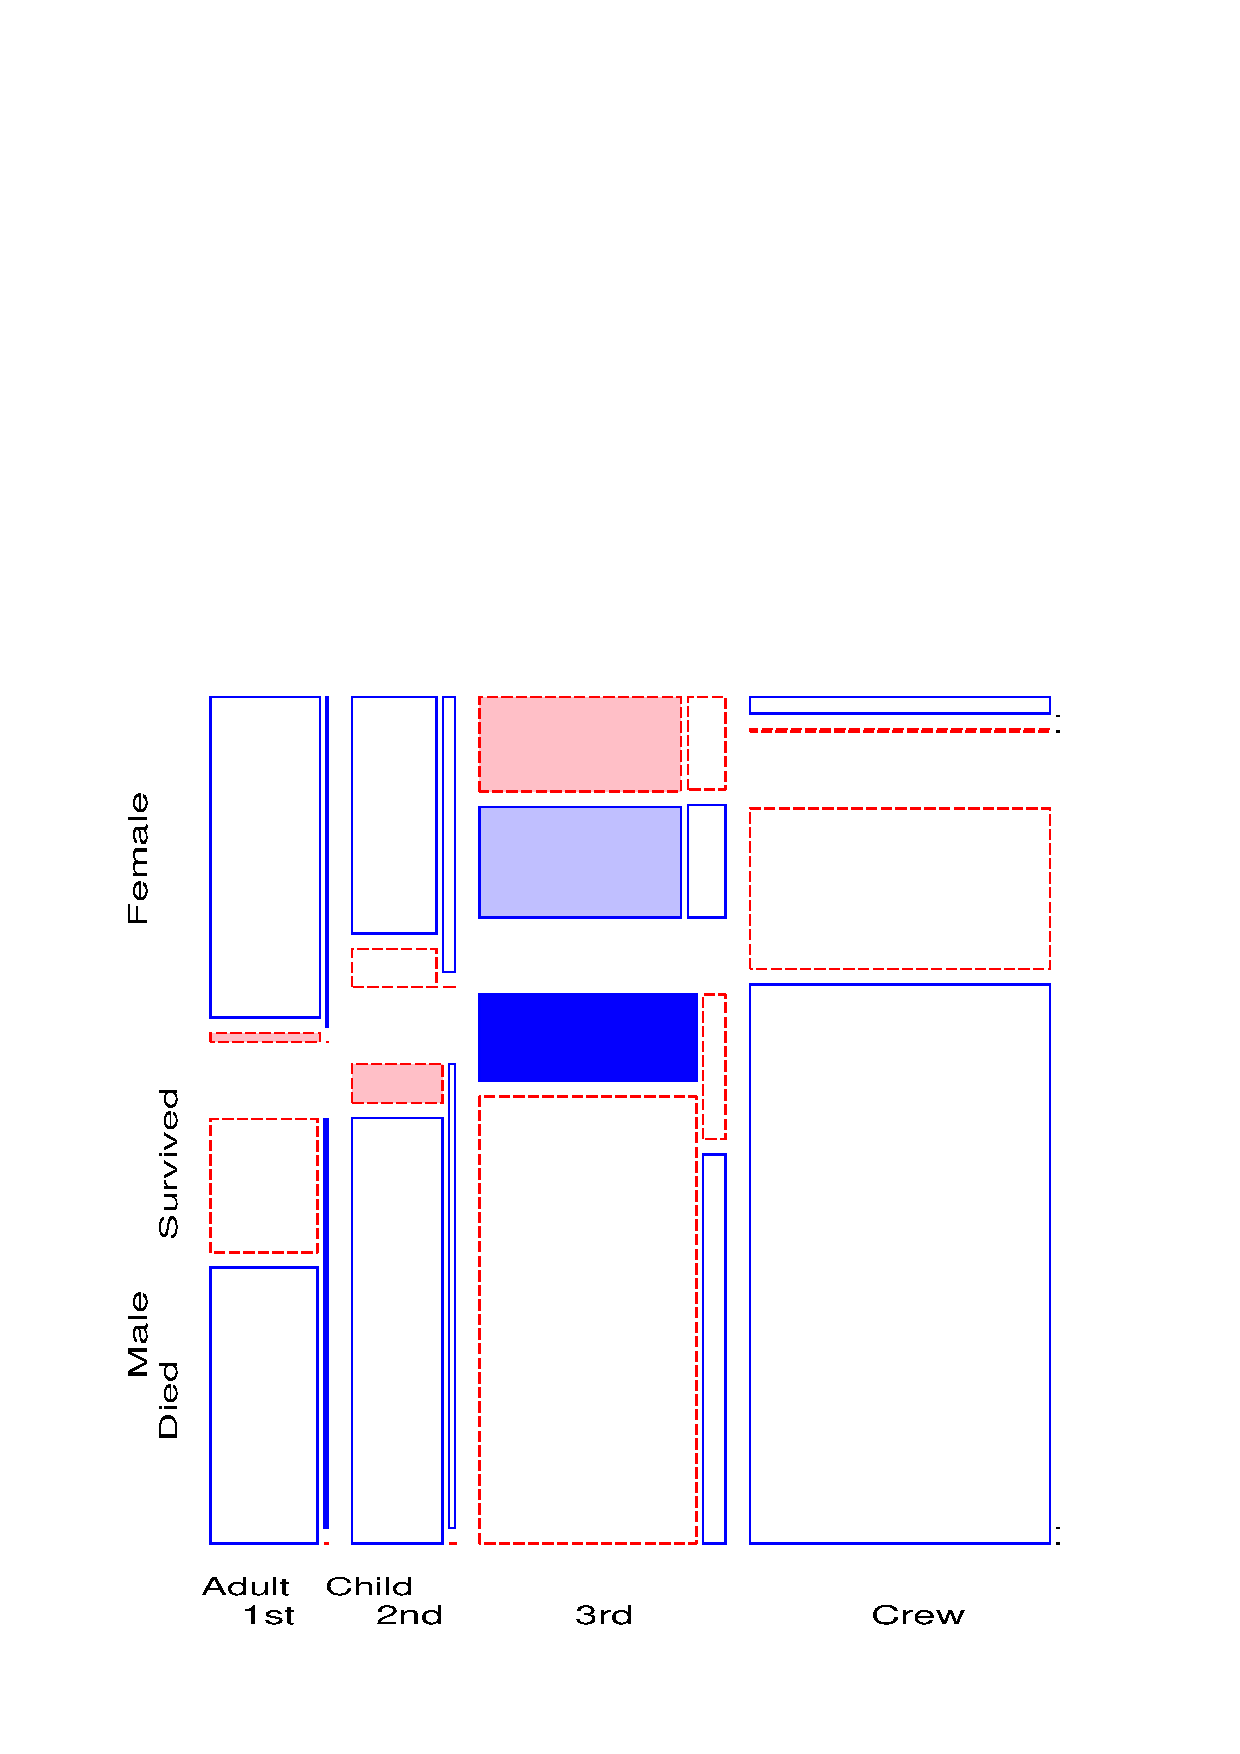
\includegraphics{ch4/fig/mostitanic5}
 }
 \subfigure[Model \LLM{CGA,CGS,CAS}]{\label{fig:mostitanic6}%
  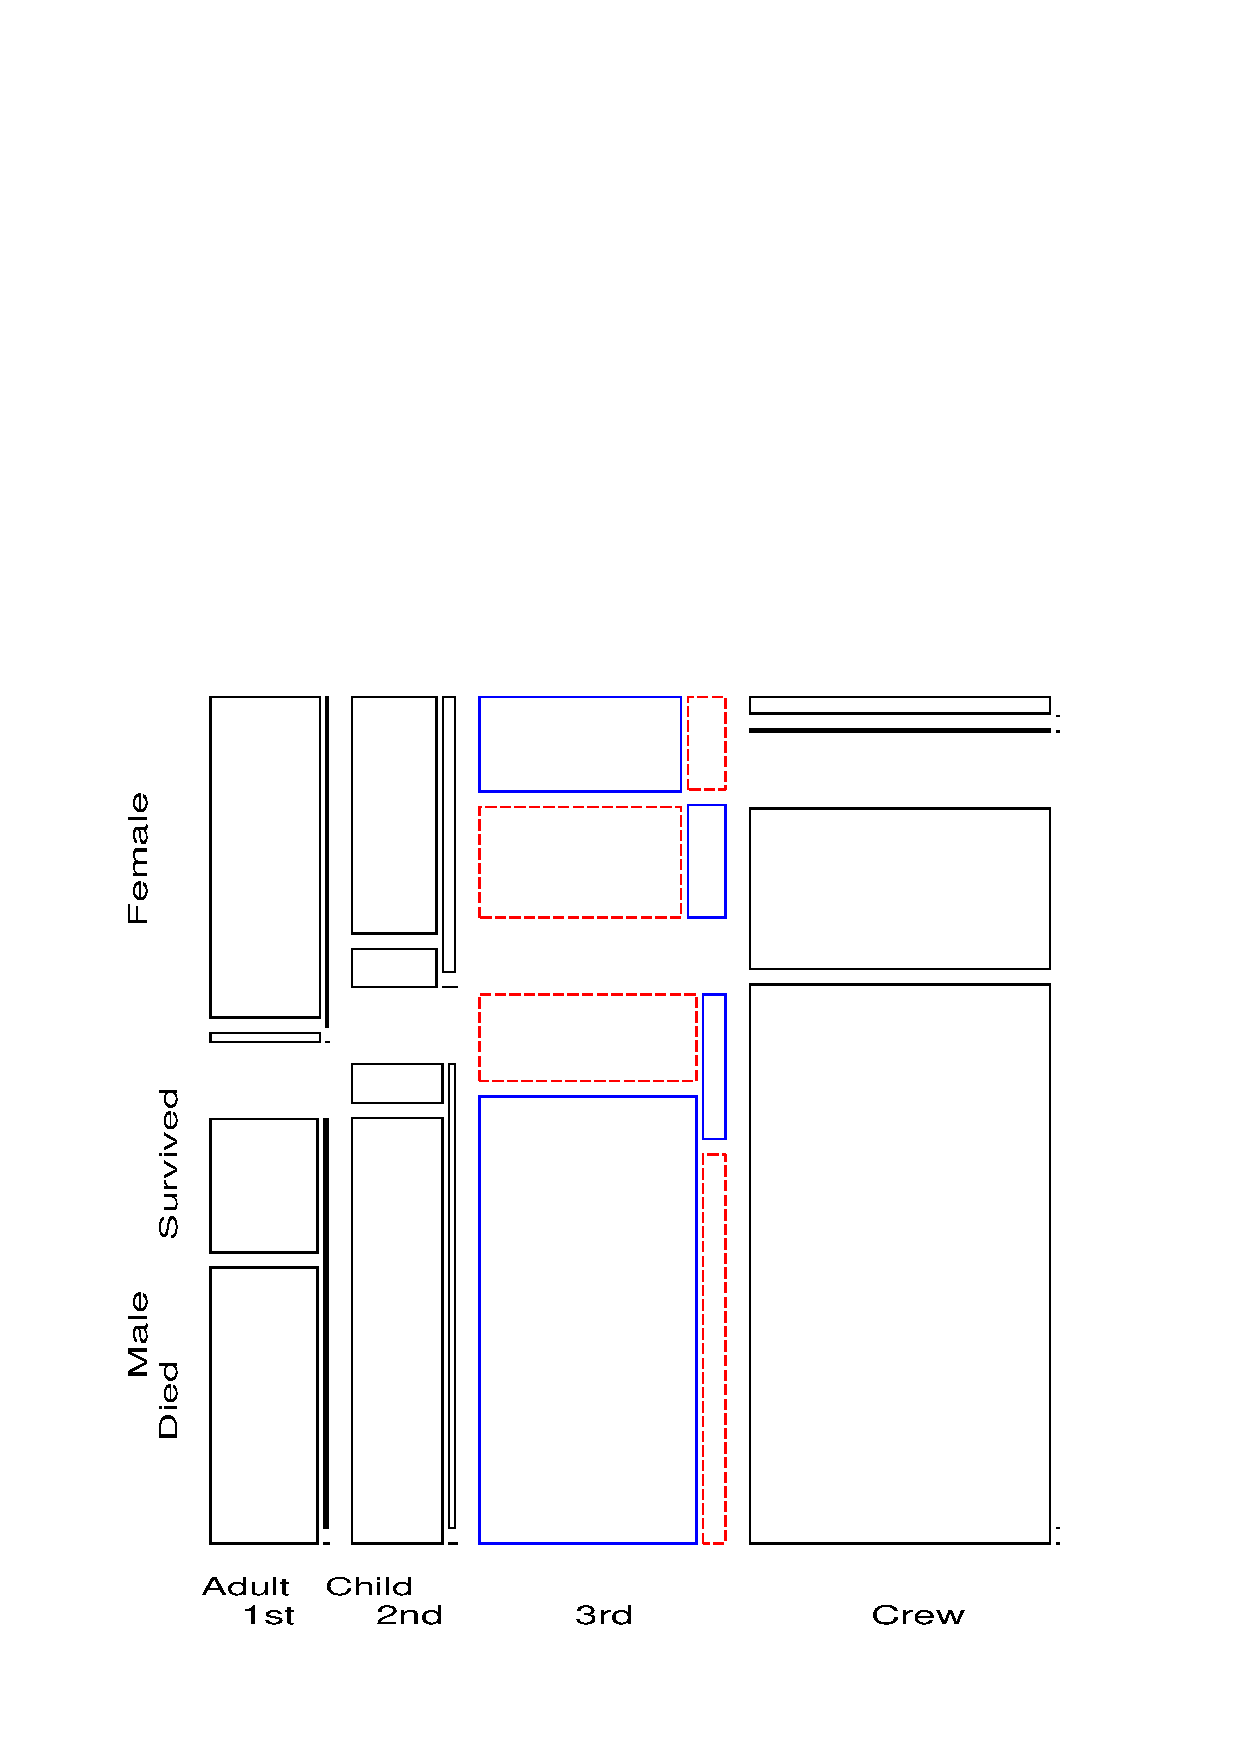
\includegraphics{ch4/fig/mostitanic6}
 }
 \end{subfigmatrix}
 \caption[Titanic data: Models with interactions]{Titanic data: Models with interactions}\label{fig:mostitanic5-6}
\end{figure}

The import of these figures is clear.
Regardless of Age and Gender, lower economic
status was associated with increased mortality; the differences due to Class
were moderated, however, by both Age and Gender.
Although women on the \emph{Titanic}
were more likely overall
to survive than men, the interaction of Class and Gender shows that
women in 3rd class did not have a significant advantage, while men in 1st class
did compared to men in other classes.  The interaction of Class and
Age is explained by the observation
that while no children in 1st or 2nd class died,
nearly two-thirds in 3rd class died;
for adults, mortality increases progressively
as economic class declines.
Hence, although the phrase ``women and
children first'' is mellifluous and appeals to our sense of Edwardian chivalry
a more adequate description might be
``women and children (according to class), then 1st class men.''
\end{Example}

\begin{frame}
  \frametitle{Partial association, Partial mosaics}
  \begin{itemize}
	\item{\large\bfseries Stratified analysis:}
      \begin{itemize*}
	  \item How does the association between two (or more) variables vary 
	  over levels of other variables?
	  \item Mosaic plots for the main variables show \emph{partial association}
	  at each level of the other variables.
%	  \item Analog of \emph{coplot} (conditioning plot) for categorical data
	  \item E.g., Hair color, Eye color \emph{BY} Sex $\leftrightarrow$ 
	  \texttt{TABLES sex * hair * eye;}
      \end{itemize*}
  \end{itemize}
\begin{center}
  \includegraphics[width=.86\dispwidth,clip]{fig/mospart3}
\end{center}

\end{frame}

\begin{frame}

  \frametitle{Partial association, Partial mosaics}
  \begin{block}{\large\bfseries Stratified analysis: conditional decomposition of $G^2$}
      \begin{itemize*}
	  \item Fit models of partial (conditional) independence, $ A \perp B \given C_k$
            at each level of (controlling for) $C$.
	  \item $\Rightarrow$ partial $G^2$s add to the overall
	  $G^2$ for conditional independence,$ A \perp B \given C$
\begin{equation*}
G^2_{A \perp B \given C} = \sum_k G^2_{A \perp B \given C(k)}
\end{equation*}
       \end{itemize*}
 \end{block}

\input{tab/haireyesex}
\end{frame}


\section{Mosaic matrices for categorical data}\label{sec:mosmat}

One reason for the wide usefulness of graphs of quantitative data
has been the
development of effective, general techniques for dealing with high-dimensional \Dsets.
The \scatmat{}
(\SSSGref{8.3.2})
shows all pairwise (marginal) views of a set of variables
in a coherent display, whose design goal is to show the interdependence
among the collection of variables as a whole.
It combines multiple views of the data
into a single display which allows detection of patterns which could
not readily be discerned from a series of separate graphs.
In effect, a multivariate \Dset\ in $p$ dimensions (variables) is shown as
a collection of $p (p-1)$ two-dimensional \scats{}, each of which is
the projection of the cloud of points on two of the variable axes.
These ideas can be readily extended to categorical data.

A \mway{} \ctab{} of $p$ categorical variables,
$A, B, C,\dots$, also contains the interdependence among the collection
of variables as a whole.  The saturated \loglin{} model, $[A B C\dots]$
fits this interdependence perfectly, but is often too complex to describe
or understand.  By summing the table over all variables except two,
$A$ and $B$, say, we obtain a two-variable (marginal) table, showing the
bivariate relationship between $A$ and $B$, which is also a projection
of the $p$-variable relation into the space of two (categorical) variables.
If we do this for all $p (p-1)$ unordered pairs of categorical variables
and display each two-variable table as a mosaic,  we have a categorical
analog of the \scatmat{}, called a
\glossterm{mosaic matrix}.
Like the \scatmat{}, the mosaic matrix can accommodate any number of
variables in principle, but in practice is limited by the resolution
of our display to three or four variables.

Mosaic matrices are produced using the \IML{}
module \texttt{mosmat}, which is called in a \PROC{IML} step as
\begin{listing}
   run mosmat(dim, table, vnames, lnames, plots, title);
\end{listing}
When there are $p$ variables in the \texttt{table}, a set of $p^2$ plots
are produced;  these include the $p (p-1)$ pairwise mosaics and a set
of $p$ panels containing the variable names (from \texttt{vnames}).
After the \IML{} step, the separate plots may be combined into one figure with the \macro{PANELS}.
The \macro{MOSMAT} provides a simple interface to these steps.

\begin{Example}[marital2]{Marital status and pre- and extramarital sex}
In \exref{ex:marital1} we examined a series of models relating marital
status to reported premarital and extramarital sexual activity and gender.
\figref{fig:mosmat5} shows the mosaic matrix for these data,
produced with the \macro{MOSMAT}, as follows:
\begin{listing}
%include catdata(marital);
%mosmat(data=marital, var=Gender Pre Extra Marital,
   vorder=Marital Extra Pre Gender, devtype=LR ADJ);
\end{listing}

If we view gender, premarital sex and extramarital sex as explanatory,
and marital status (divorced vs.\  still married) as the response,
then the mosaics in row 1 (and in column 1)%
%
\footnote{Rows and columns in the mosaic matrix are identified
as in a table or numerical matrix, with row 1, column 1 in the upper left corner.}
%
shows how marital status
depends on each predictor marginally.
The remaining panels show the relations within the set of explanatory
variables.

%% one figure
\begin{figure}[htb]
  \centering
  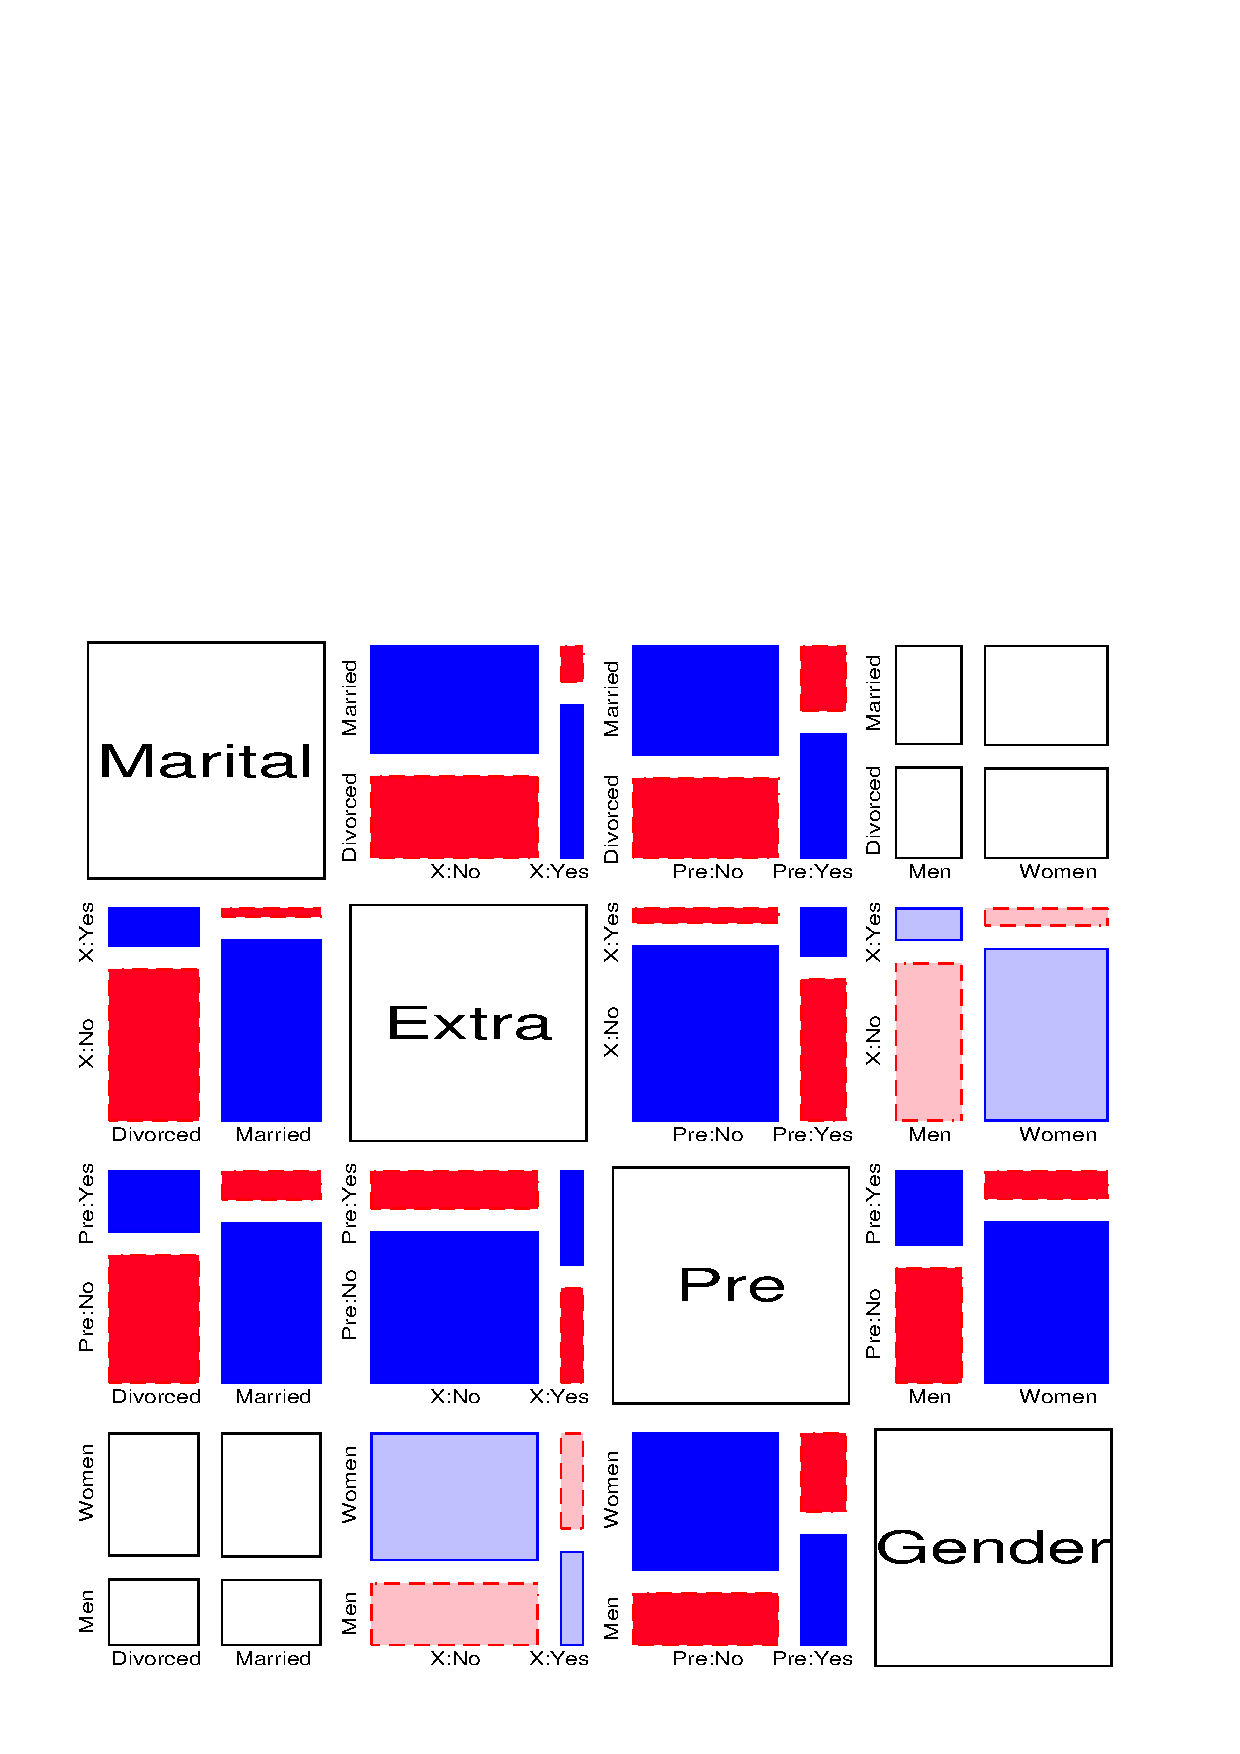
\includegraphics[scale=.8]{ch4/fig/mosmat5m}
  \caption[Mosaic matrix for marital status data]{Mosaic matrix for marital status data.
  Each panel shows the marginal relation,
fitting an independence model between the row and column variable, collapsed over other variable(s).}%
  \label{fig:mosmat5}
\end{figure}

Thus, we see in row 1, column 4, that marital status is independent
of gender (all residuals equal zero, here), by design of the data
collection.  In the (1, 3) panel, we see that reported premarital sex
is more often followed by divorce, while non-report is more prevalent
among those still married.  The (1, 2) panel shows a similar, but stronger relation between extramarital sex and marriage stability.  These
effects pertain to the associations of P and E with marital status---%
the terms [PM] and [EM] in the \loglin{} model.  We saw earlier that
an interaction of P and E (the term [PEM]) is required to fully account for these data.  This effect is not displayed in \figref{fig:mosmat5}.

Among the background variables (the \loglin{} term [GPE]), the (2, 3) panel shows a strong relation
between premarital sex and subsequent extramarital sex, while
the (2, 4) and (3, 4) panels show that men are far more likely to report
premarital sex than women in this sample, and also more likely to
report extramarital sex.
\end{Example}

\begin{Example}[berkeley4]{Berkeley admissions}
\figref{fig:mosmat9a} shows the pairwise marginal
relations among the variables
Admit, Gender and Department in the Berkeley
data which were examined earlier (\exref{ex:berkeley1}) in fourfold displays
(\figref{fig:fourfold13} and \figref{fig:pie2x2b}).
This figure is produced using the \macro{MOSMAT} as shown below.
The \macro{TABLE} is first used to recode the factor variables
to more meaningful character labels.
%% input: /Users/friendly/sasuser/mosaics/mosmat9m.sas
%% last modified: 19-Jul-99 10:44
\begin{listing}
%include goptions;
goptions hsize=7 in vsize=7 in;
libname mosaic '~/sasuser/mosaics';
 
%include catdata(berkeley);
proc format;
   value admit 1="Admit" 0="Reject" ;
   value dept  1="A" 2="B" 3="C" 4="D" 5="E" 6="F";
   value $sex  'M'='Male'   'F'='Female';
%table(data=berkeley, var=Admit Gender Dept, weight=freq, char=Y,
        format=admit admit. gender $sex. dept dept., 
        order=data, out=berkeley);

%mosmat(data=berkeley, vorder=Admit Gender Dept, sort=no, htext=3.5);
\end{listing}


The panel in row 2, column 1
shows that Admission and Gender are
strongly associated marginally, as we saw in \figref{fig:fourfold13},
and overall, males are more often admitted.
The diagonally-opposite panel (row 1, column 2) shows the
same relation, splitting first by gender.%
%
\footnote{Note that this is different than just the transpose or interchange
of horizontal and vertical dimensions as in the \scatmat{},
because the mosaic display splits the total frequency first by the horizontal
variable and then (conditionally) by the vertical variable.
The areas of all corresponding tiles are the same in each diagonally
opposite pair, however, as are the
residuals shown by color and shading.}
%
\begin{figure}[!htb]
  \centering
  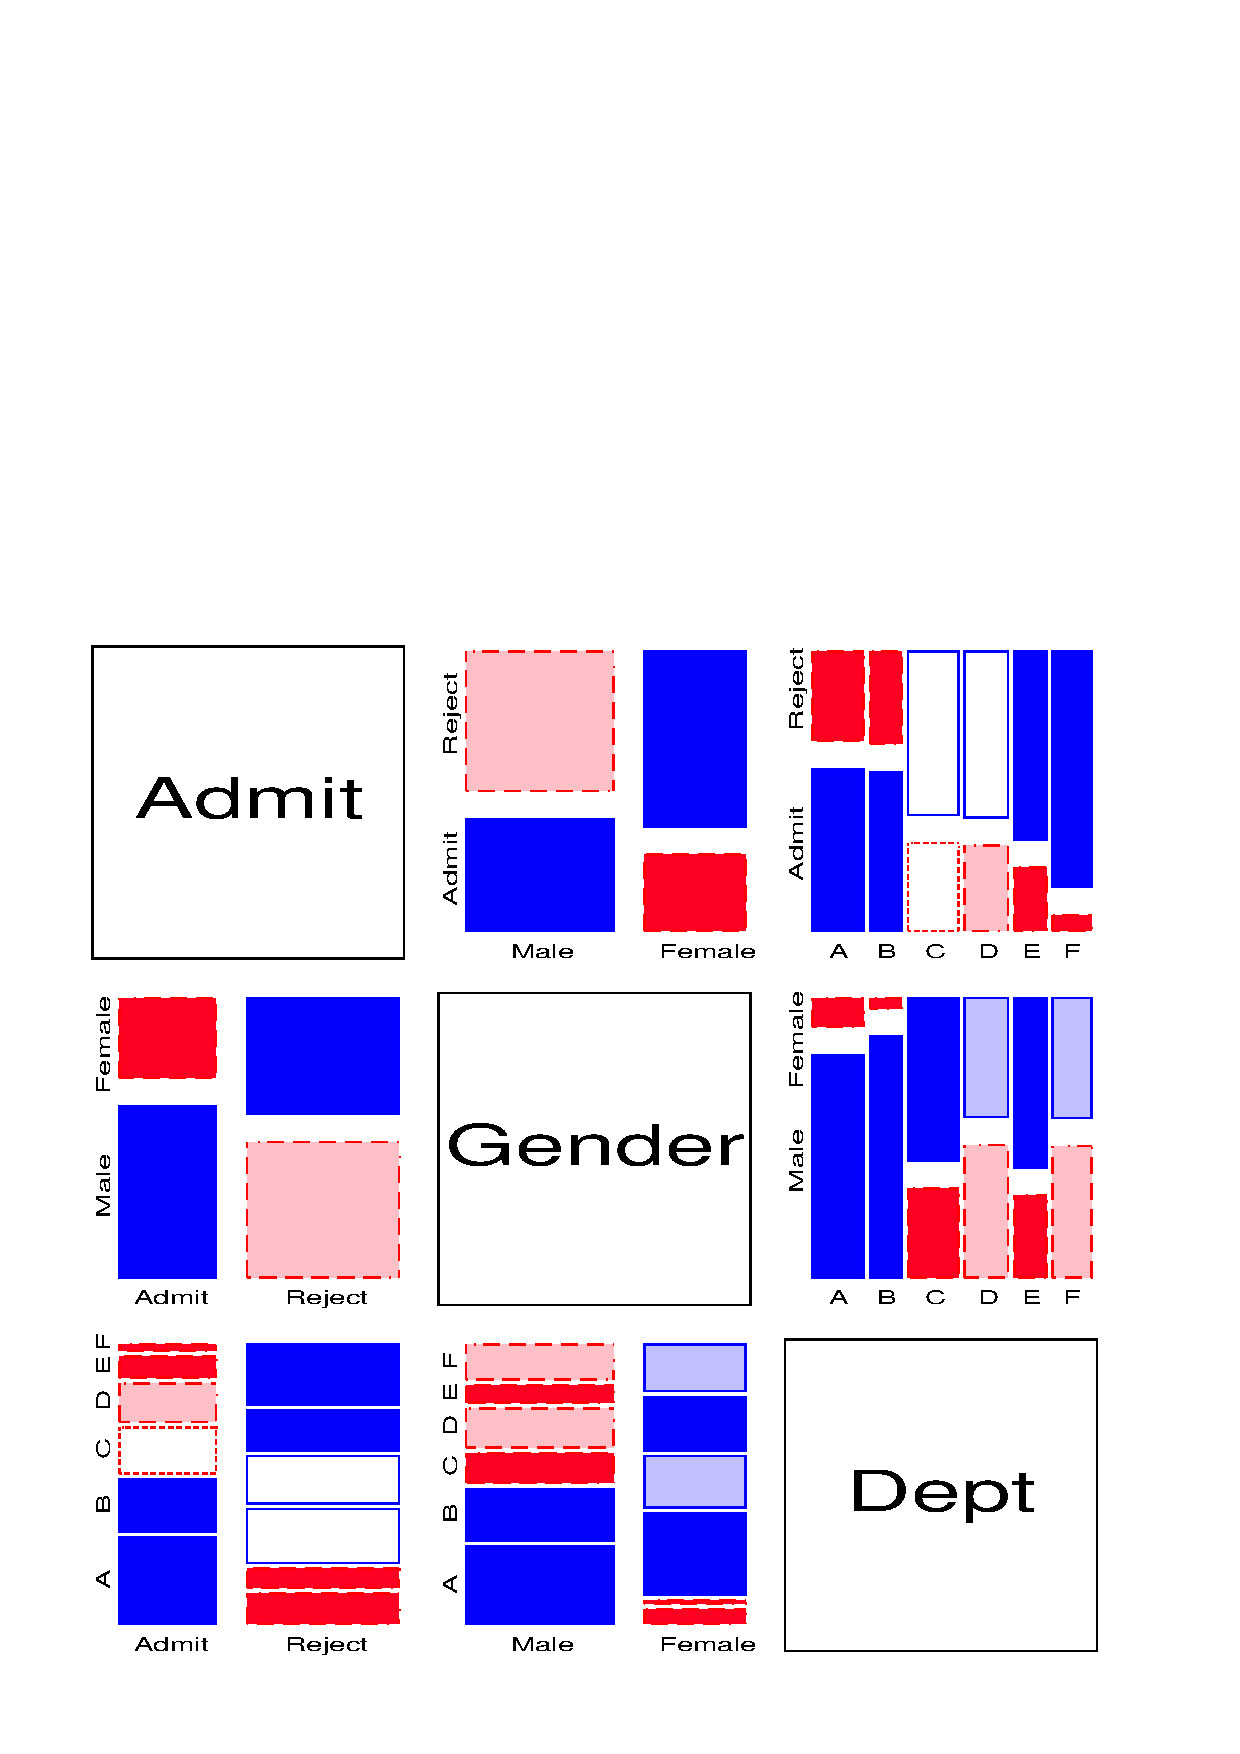
\includegraphics[scale=.8]{ch4/fig/mosmat9a}
  \caption[Marginal mosaic matrix of Berkeley
admissions]{Mosaic matrix of Berkeley
admissions, showing bivariate marginal relations.}\label{fig:mosmat9a}
\end{figure}

The panels in the third column (and third row)
illuminate the explanation for the paradoxical
result (see \figref{fig:pie2x2b}) that, within all but department A,
the likelihood of admission is equal for men and women,
yet, overall, there appears to be a bias in favor of admitting men
(see \figref{fig:fourfold13}).
The (1,3) and (3, 1) panels show
the marginal relation between Admission and Department; departments A and B have the greatest
overall admission rate, departments E and F the least.
The (2, 3) panel shows that men apply in much greater numbers to
departments A and B, while women apply in greater numbers to
the departments with the lowest overall rate of admission.
\end{Example}

\subsection{Conditional mosaic matrices}\label{sec:condmat}

We need not show the marginal relation between
each pair of variables in the mosaic matrix.
A conditional mosaic matrix fits a model of conditional independence
between each row and column, controlling for one or more of the other
variables.   \citet{Friendly:99b} gives further details and describes
analogous displays for quantitative data.

\begin{Example}[berkeley4b]{Berkeley admissions}
For example, \figref{fig:mosmat9b} shows all pairwise \emph{conditional}
relations among the variables Gender, Dept, Admit in the Berkeley data.
All panels show the \emph{same} observed frequencies in the three-way table
by the areas of the tiles,
but each fits a model of conditional independence between the row and
column variable, with the remaining variable controlled.
Thus, the shading in the (1,2) and (2,1) panels show the fit of the model
[Admit, Dept] [Gender, Dept],
which asserts that Admission and Gender are independent, given (controlling
for) Department.  Except for Department A, this model fits quite well,
again indicating lack of gender bias.
The (1,3) and (3,1) panels show the relation between admission and department
controlling for gender, highlighting the differential admission rates
across departments.
\begin{figure}[!htb]
  \centering
  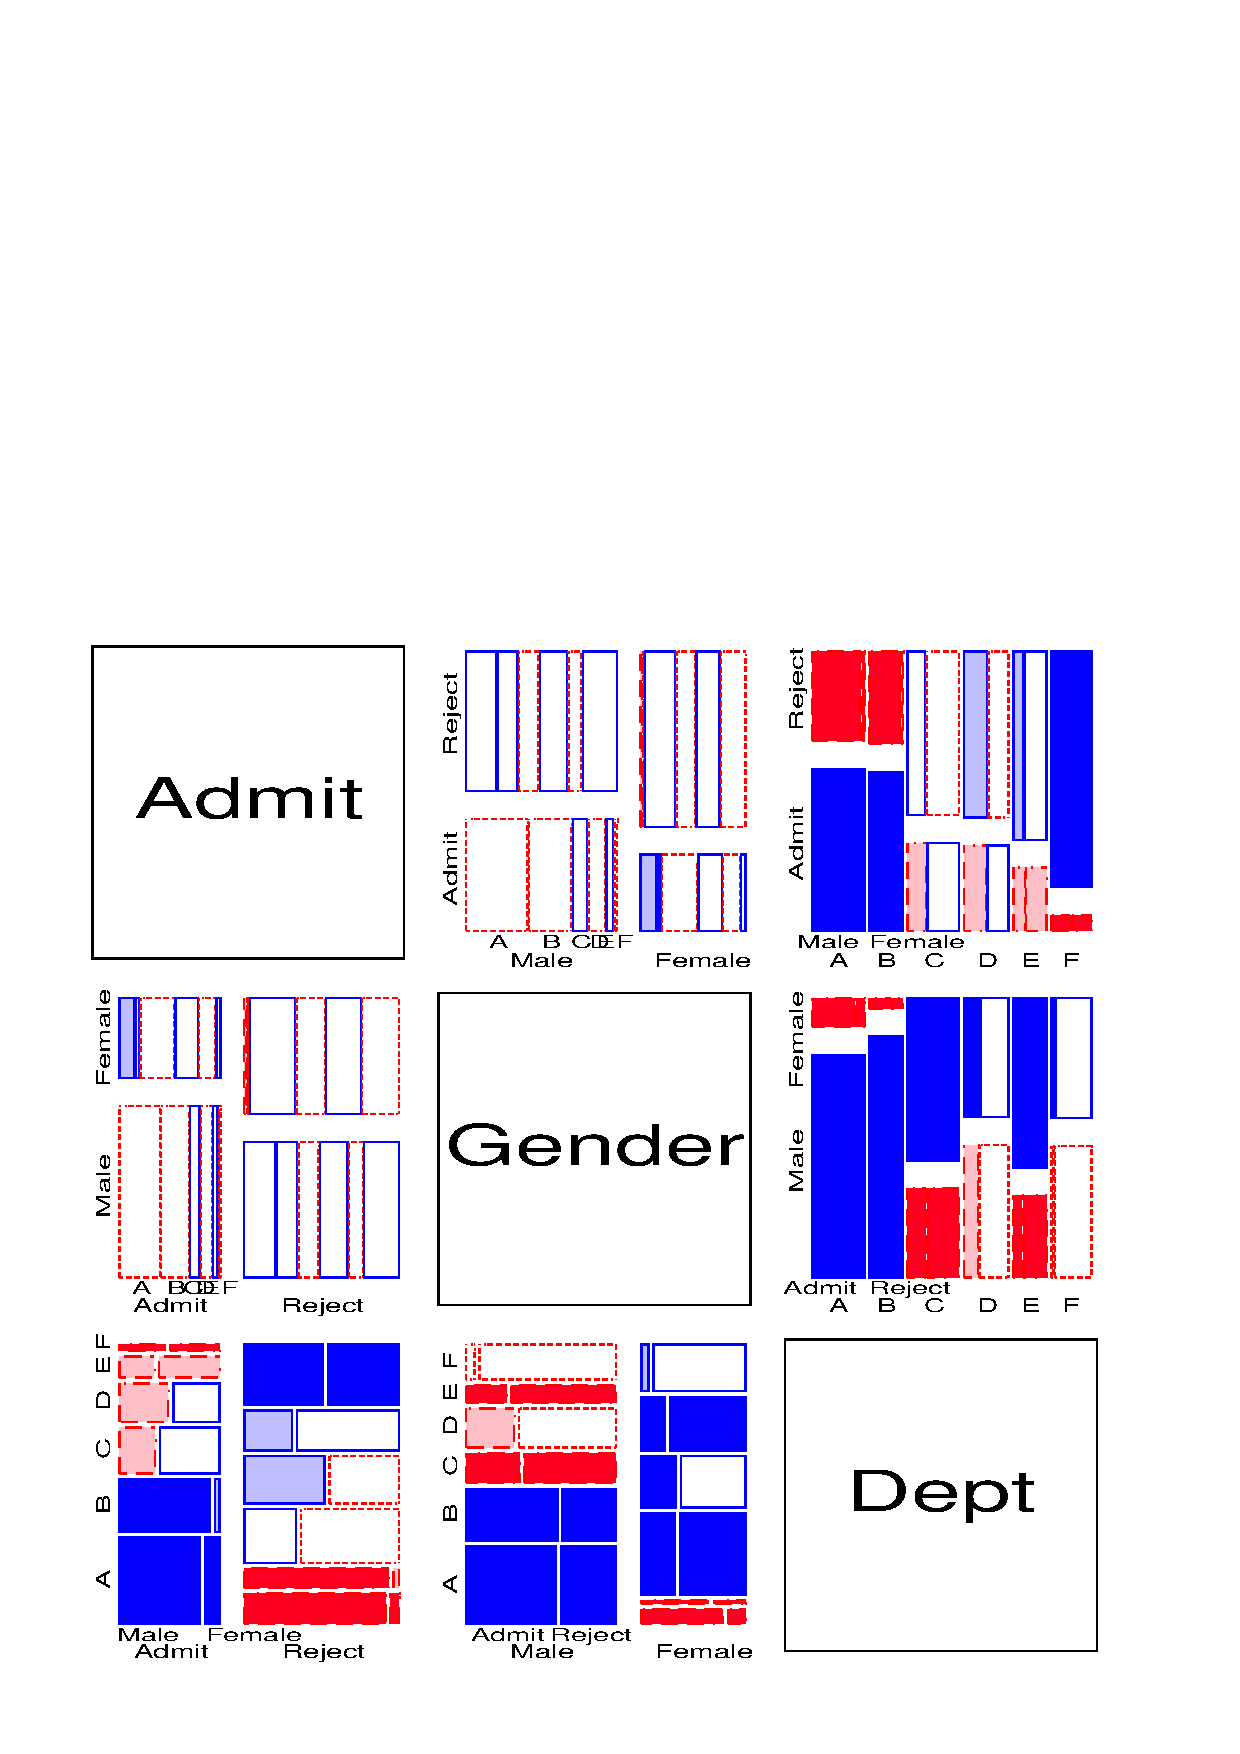
\includegraphics[scale=.8]{ch4/fig/mosmat9b}
  \caption[Conditional mosaic matrix of Berkeley
admissions]{Conditional mosaic matrix of Berkeley
admissions.  Each panel shows the conditional relation,
fitting a model of conditional independence between the row and column variable, controlling for other variable(s).}\label{fig:mosmat9b}
\end{figure}

Conditional mosaic matrices are produced with the \macro{MOSMAT}
by specifying \texttt{CONDIT} as the \mparm{fittype}{MOSMAT}.
The parameter \texttt{plots=3} specifies that each panel in the
display contains the three-way mosaic plot for the data.
%% input: /Users/friendly/sasuser/mosaics/mosmat9m.sas
%% last modified: 19-Jul-99 10:44
\begin{listing}
%mosmat(data=berkeley, vorder=Admit Gender Dept, sort=no, htext=3.5,
   plots=3, fittype=CONDIT);
\end{listing}

\end{Example}

\section{Showing the structure of \loglin{} models}\label{sec:mosaic-struc}
The mosaic display can also be used to illuminate the relations among
variables in a \ctab{} which are represented in various \loglin{} models,
a point described by \citet{TheusLauer:99}.
Each of the model types depicted in \tabref{tab:hyp3way} has, in fact,
a characteristic shape and structure in a mosaic display. This,
in turn, leads to a clearer understanding of the structure which appears
in real data when a given model fits, the relations among the models,
and the use of mosaic displays.

%%
%% Table struc written by md2tex 29MAY98 08:46
%%
\begin{table}[htb]
 \caption{A $2 \times 2 \times 2$ table (artificial data)}
 \label{tab:struc}
 \begin{center}
  \begin{tabular}{|l|rrrr|r|}
   \hline
% & \multicolumn{4}{c|}{\bfseries\large B} & \rule{0in}{2.5ex}\\
 & \multicolumn{2}{c|}{B1} & \multicolumn{2}{c|}{B2} &  \\\cline{2-5}
% & \multicolumn{4}{c|}{\bfseries\large A} & \rule{0in}{2.5ex}\\
{\bfseries\large C} & A1 & A2 & A1 & A2& {\bfseries\large Total} \\
   \hline
C1   &     6 &    10 &   312 &    44 &   372 \\
C2   &    37 &    31 &   192 &    76 &   336 \\
   \hline
\rule{0in}{2.5ex}{\bfseries\large Total} &   43 &    41 &   504 &   120 &   708 \\
   \hline
  \end{tabular}
 \end{center}
\end{table}

To show this, we use artificial data for a $2 \times 2 \times 2$ table
shown in \tabref{tab:struc}.
We can force such a table to conform to any \loglin{} model
(e.g., $H_1$ -- $H_4$)
simply by finding the expected frequencies under that model
and constructing a mosaic depicting the expected frequencies.

\subsection{Mutual independence}
For example, to show the structure of a table which fits
mutual independence, $H_1$, use the \FUNC{IPF} to find the
fitted values, \texttt{fit}, as

\begin{verbatim}
proc iml;
   table = { ... };
   dim= {2 2 2};
   vnames={A B C};
   lnames = {'A1' 'A2',  'B1' 'B2',  'C1' 'C2'};

   config = {1 2 3};
   call ipf(fit,status,dim,table,config);
   fittype='MUTUAL';
   print fittype config[f=4.] fit[f=7.2];
\end{verbatim}
The fitted frequencies then have the same one-way margins as the
data in \tabref{tab:struc}, but have no two-way or higher associations.
We then display a mosaic for the \emph{fitted frequencies}
to see what mutual independence looks like in a three-way table.
\begin{output}
   FITTYPE  CONFIG             FIT
   MUTUAL      1   2   3     34.10   10.04  253.31   74.56
                             30.80    9.07  228.79   67.34
\end{output}
What you see in a mosaic display depends, in large measure, on the order in
which the table variables are entered.
For three variables there are $3!=6$ possible orders;  conveniently,
they are all shown in the mosaic matrix.
In this display we show the three-way mosaic (\texttt{plots=3;})
for each pair of variables, using the fitted values as the ``data.''
The statements below produce \figref{fig:mosfit-1}.
\begin{figure}[htb]
  \centering
  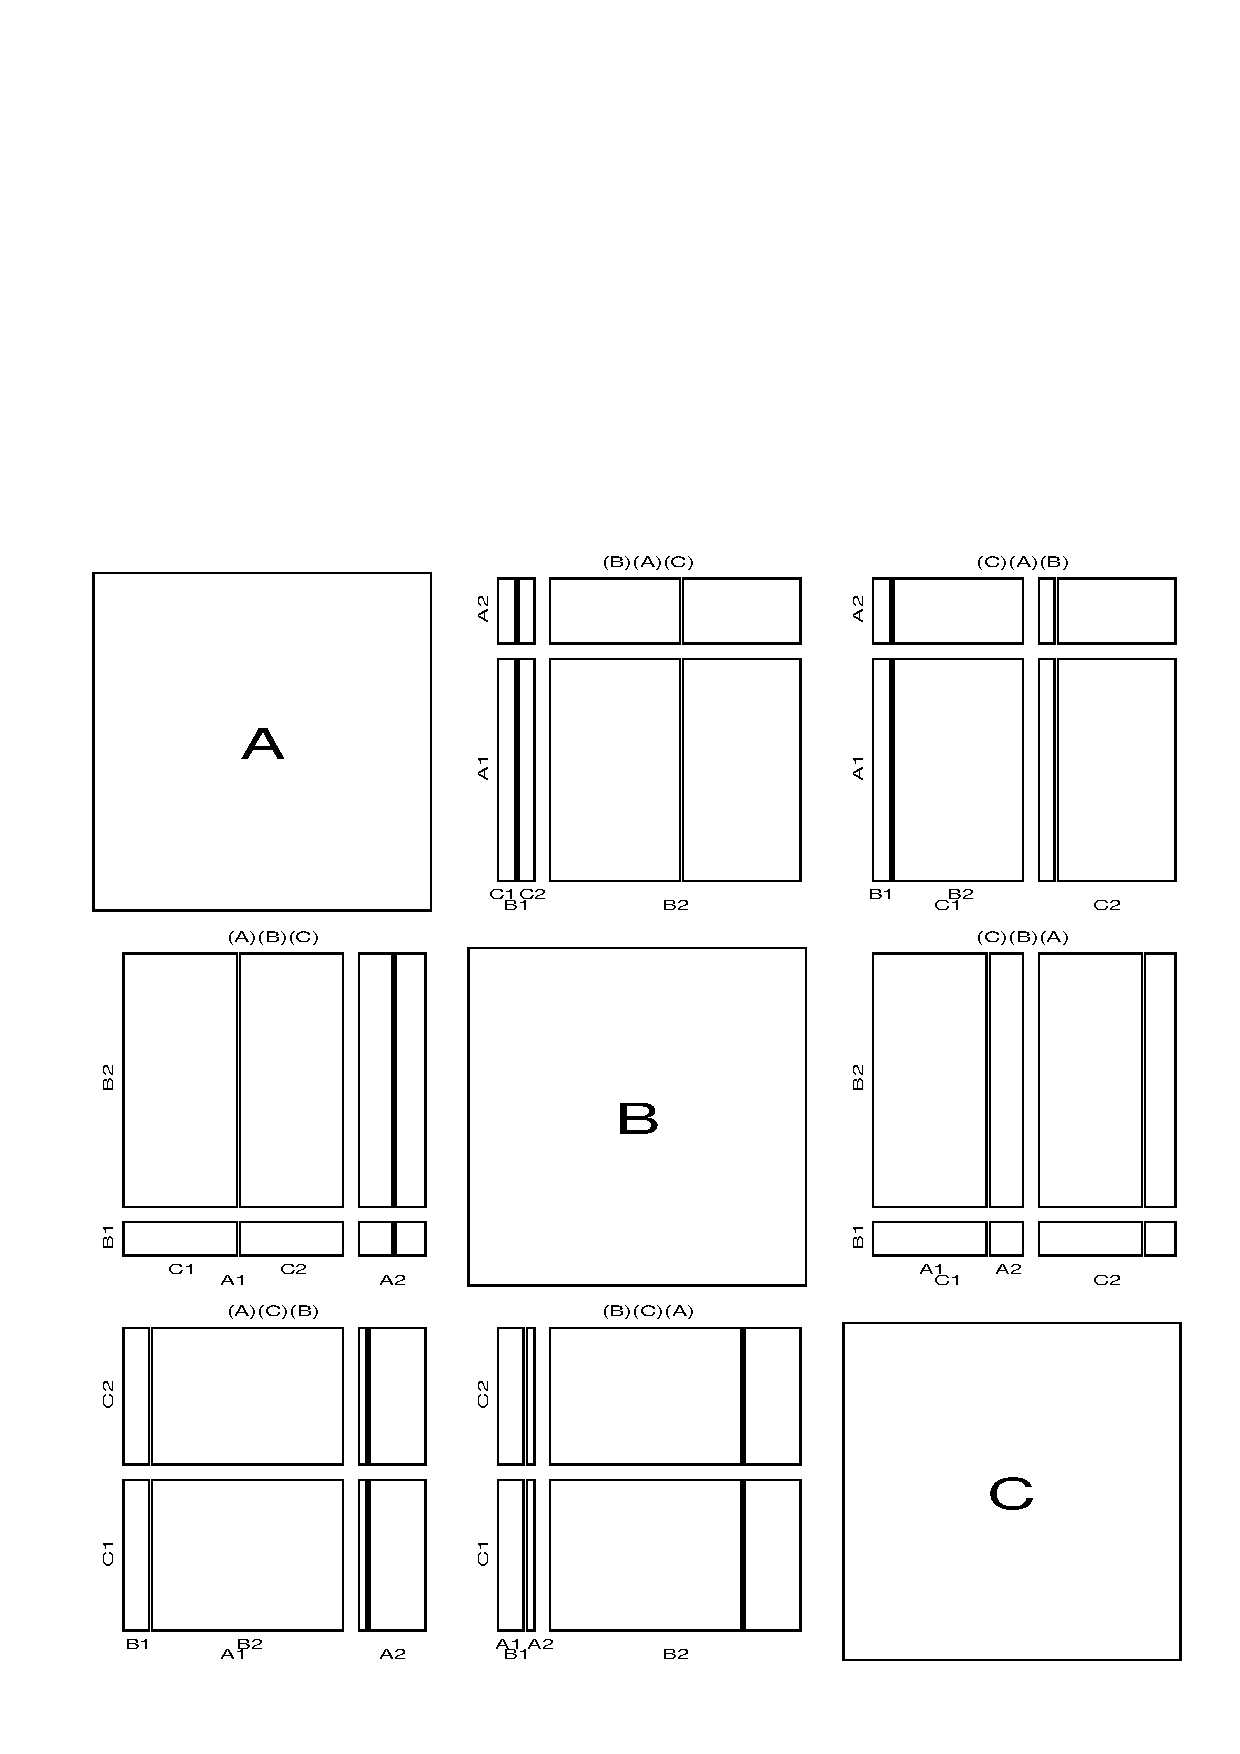
\includegraphics[scale=.6]{ch4/fig/mosfit-1}
  \caption[Mosaic matrix for mutual independence]{Mosaic matrix for mutual independence.  All panels show marginal and conditional independence among all three pairs of variables.}%
  \label{fig:mosfit-1}
\end{figure}

\begin{verbatim}
   plots=3;
   title=fittype+'&MODEL';
   space={12 5};
   run mosmat(dim, fit, vnames, lnames, plots, title);
quit;
%panels(rows=3, cols=3, equate=Y, order=down);
\end{verbatim}


In this figure the same data are shown in all the off-diagonal panels
and the mutual independence model was fitted in each case, but with the
table variables permuted.  All residuals are exactly zero in all cells,
by construction.
We see that in each view, the four large
tiles, corresponding to the first two variables align, indicating
that these two variable are marginally independent.
For example, in the $(1,2)$ panel, $A$ and $B$ are independent, collapsed
over variable $C$.

Moreover, comparing the top half to the bottom half
in any panel we see that the divisions by the third variable
are the same for both levels of the second variable.
In the $(1, 2)$ panel, for example, $A$ and $C$ are independent at
$B1$, and also independent at  $B2$.
This means, though, that $A$ and $B$ are conditionally independent
given $C$ ($A \perp B \given C$).
Because this holds in all six panels, we see that mutual independence
is equivalent to \emph{all pairs} of variables being conditionally
independent, given the remaining one,  ($X \perp Y \given Z$) for all
permutations of variables.

\subsection{Joint independence}
The model of joint independence, $H_2: \: (A, B) \perp C$, or
equivalently, the \loglin{} model $[A B][C]$
may be visualized similarly by the mosaic matrix in \figref{fig:mosfit-21},
in which the data were replaced by fitted values under this model.
\begin{figure}[htb]
  \centering
  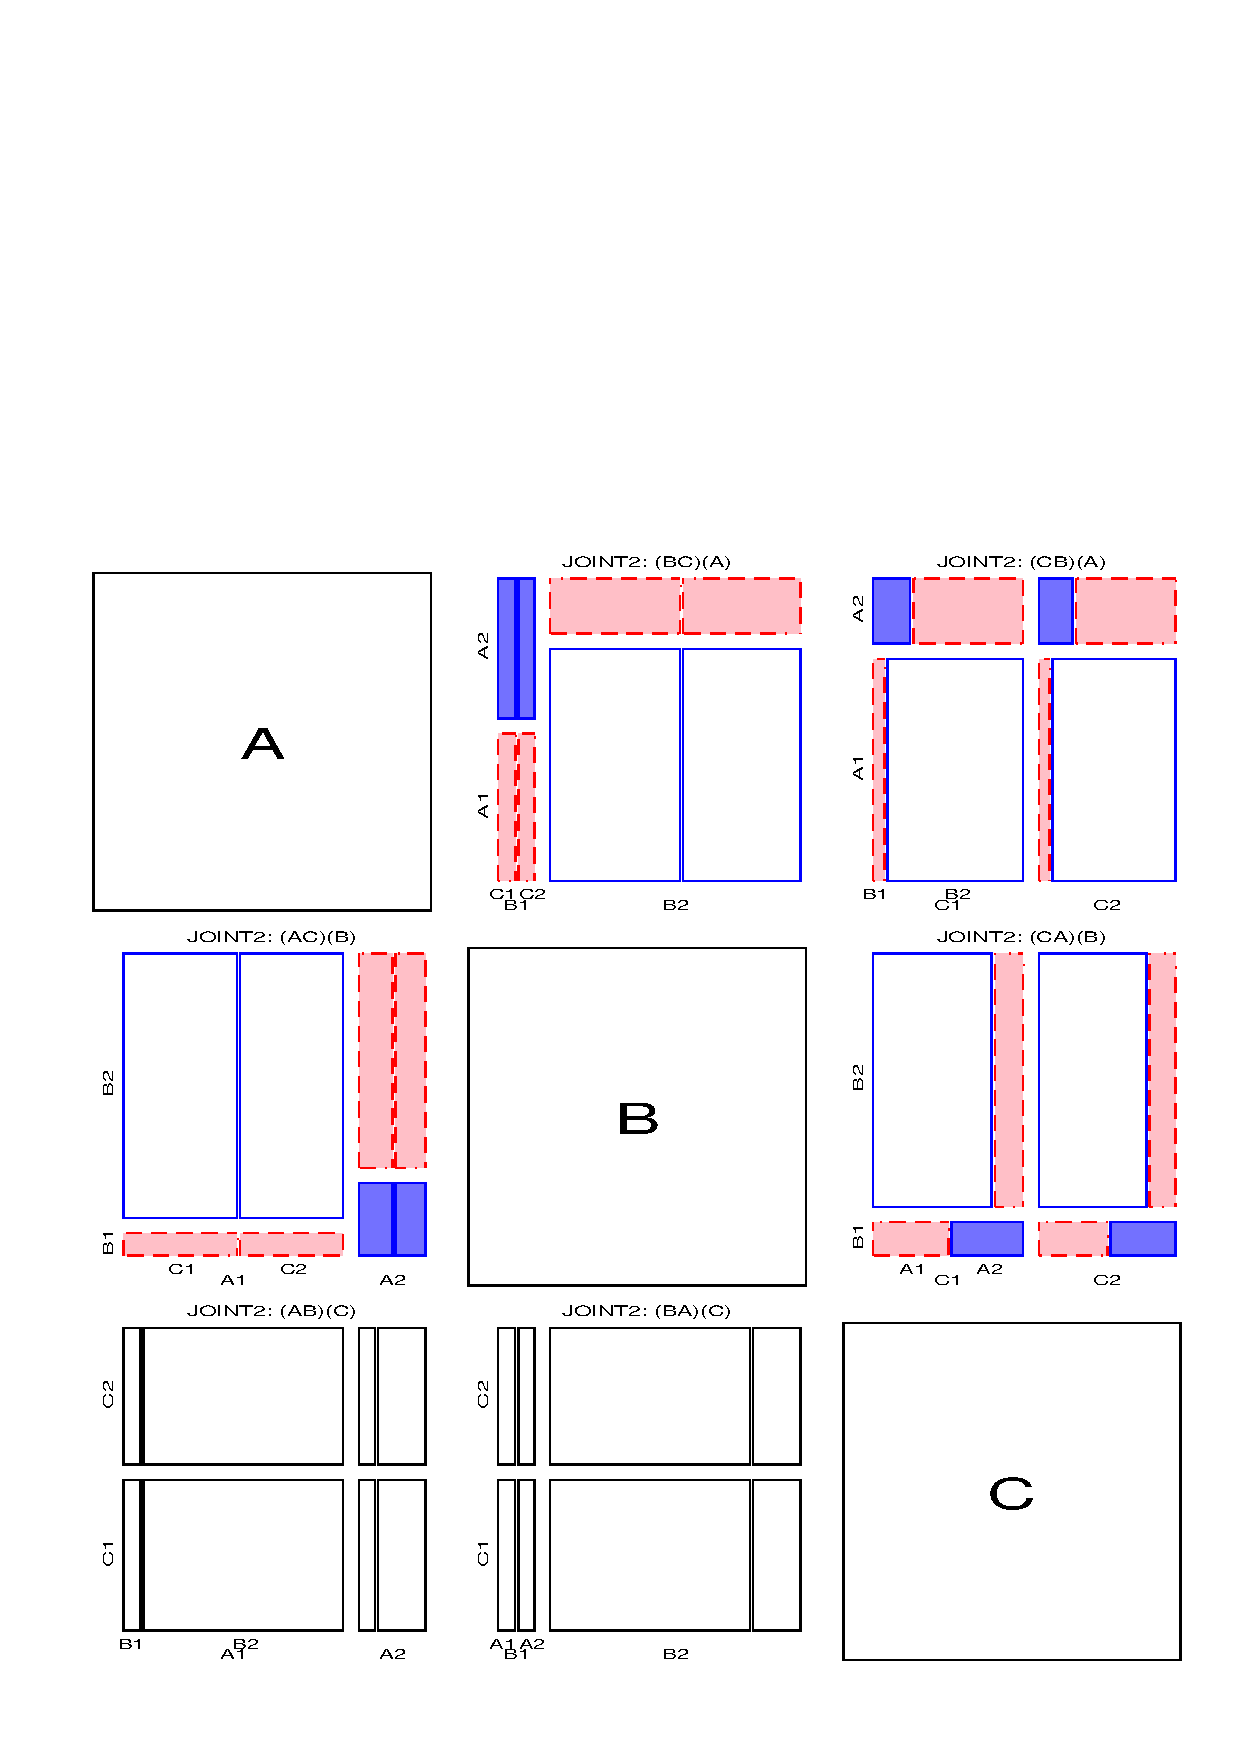
\includegraphics[scale=.6]{ch4/fig/mosfit-21}
  \caption[Mosaic matrix for joint independence]{Mosaic matrix for joint independence.  The bottom row shows that $A$ and $B$ are each independent
 of $C$, and  also
conditionally independent of $C$}%
  \label{fig:mosfit-21}
\end{figure}
\begin{verbatim}
   ...
   config = t({1 2, 3 0});
   call ipf(fit,status,dim,table,config);
   fittype='JOINT2';
   ...
\end{verbatim}
which gives these fitted frequencies.
\begin{output}
   FITTYPE  CONFIG        FIT
   JOINT2      1   3    22.59   21.54  264.81   63.05
               2   0    20.41   19.46  239.19   56.95
\end{output}
The \texttt{fittype='JOINT2';} specifies that in each panel the fitted model
is that wherein the first and third variable are independent of the second.
Now, in \figref{fig:mosfit-21}, the same model is fit in both panels in
each row,  but the second, distinguished variable differs from
row to row.

We see in row 3, where $C$ is the second variable, that $C$ is independent
of $A$, and also independent of $B$, and these models have residuals
equal to zero.
The models fit in the other four panels have non-zero residuals.
However, the $(1, 2)$ and $(2, 1)$ panels show that
$B \perp C \given A$, and $A \perp C \given B$, respectively, because
the top and bottom portions are both divided equally by the third table
variable.
This relation does not hold, however, in the $(1, 3)$ and $(2, 3)$ panels.
Thus, joint independence implies that conditional independence hold
as well, but only for the two variables which enter jointly.

The appearance in the bottom row of \figref{fig:mosfit-21}
that $A$ and $B$ are marginally independent, is
misleading, because the $AB$ association is fit exactly in these models.
To see the marginal relations under $[A B][C]$ explicitly,
we can just change the \texttt{plots} value to \texttt{plots=2;},
so that the model of (marginal) independence is fit to the first two
variables in each panel and only these variables are displayed.
This plot appears in \figref{fig:mosfit-22}, and shows
clearly that $A$ and $B$ are each marginally independent of $C$,
but not of each other.
\begin{figure}[htb]
  \centering
  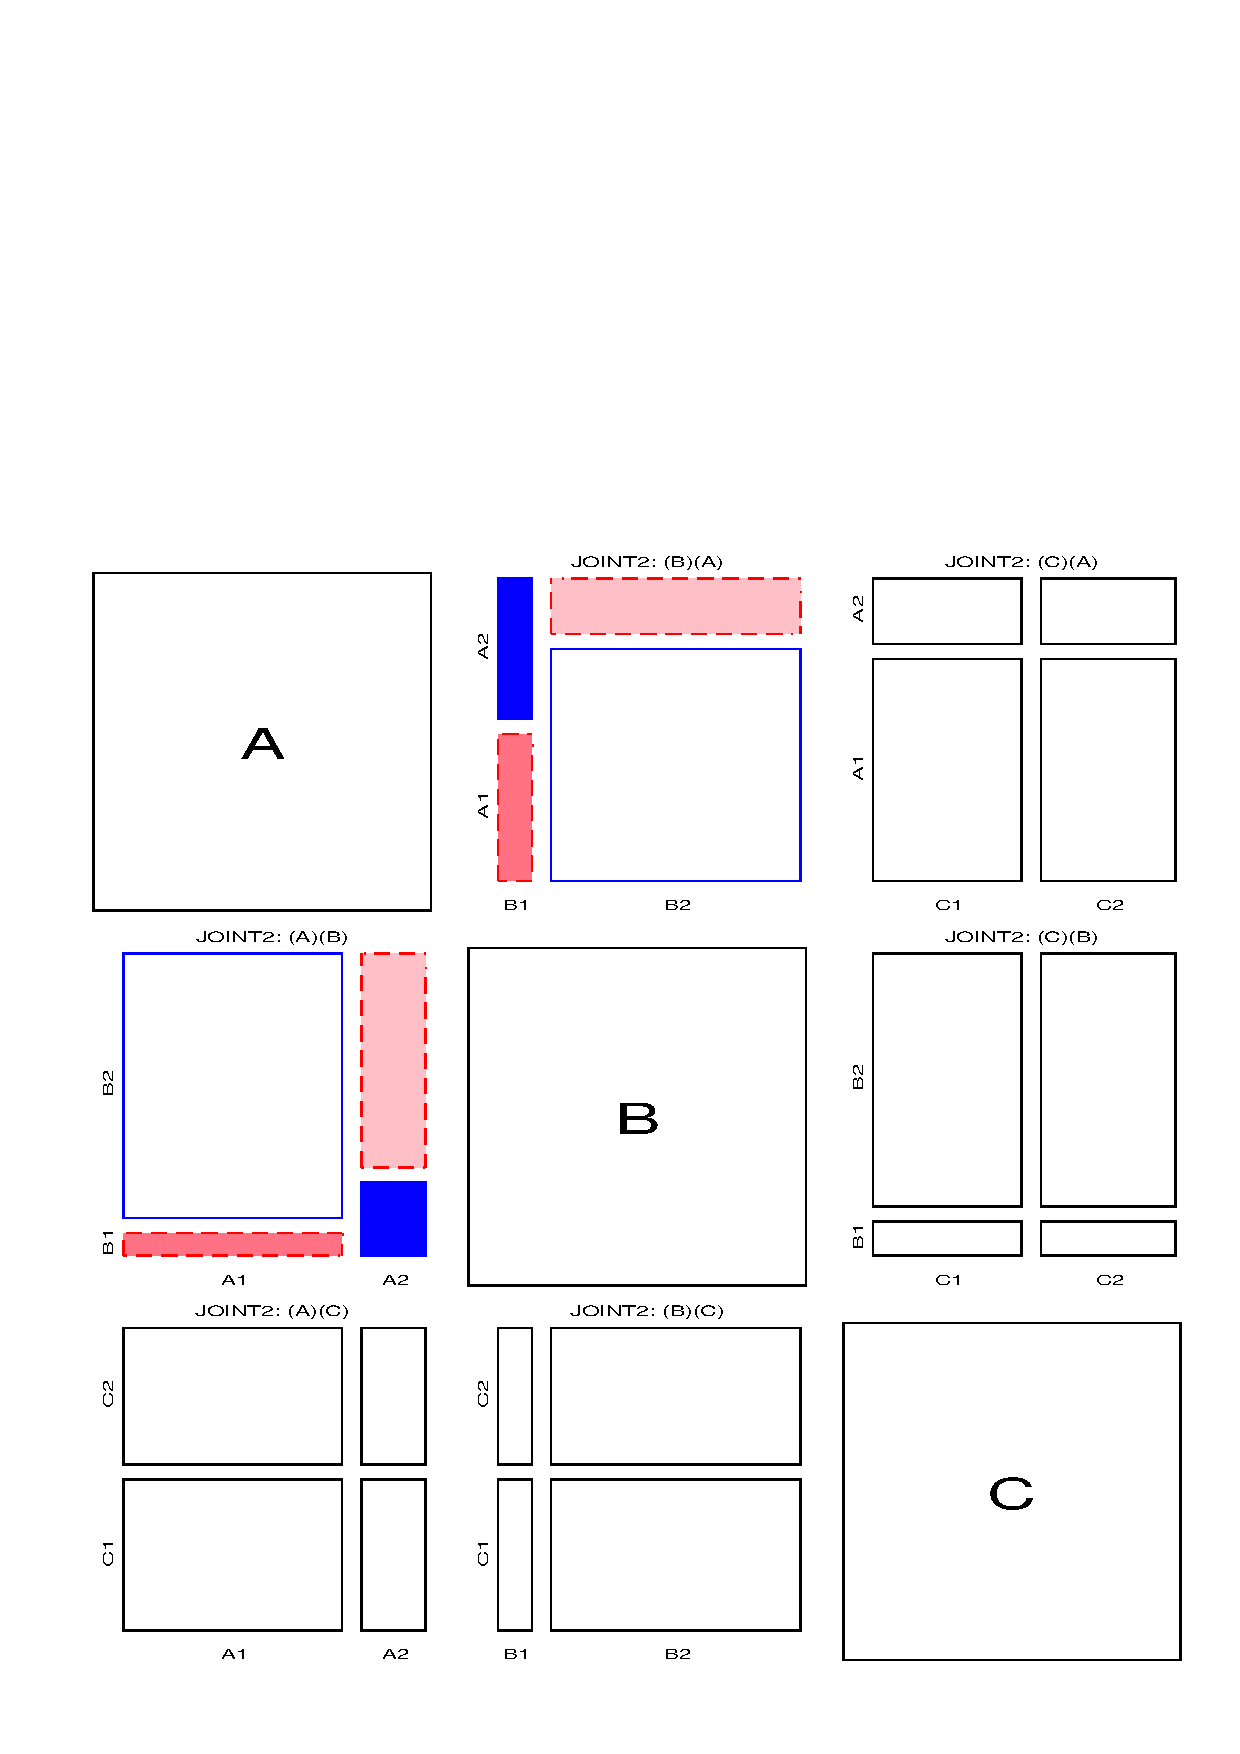
\includegraphics[scale=.6]{ch4/fig/mosfit-22}
  \caption[Marginal relations under joint independence]{Marginal relations under joint independence.  $A$ and $B$ are each marginally independent
 of $C$}%
  \label{fig:mosfit-22}
\end{figure}

\subsection{Conditional independence}
For conditional independence, $H_3: \: A  \perp B \given C$,
or $[A C][B C]$, we proceed similarly,  using
\begin{verbatim}
   config = t({1 2, 2 3});
   call ipf(fit,status,dim,table,config);
   fittype='CONDIT1';
   ...
\end{verbatim}
to obtain frequencies which fit this model exactly.
The resulting three-way mosaic matrix is shown in \figref{fig:mosfit-3}.
\begin{figure}[htb]
  \centering
  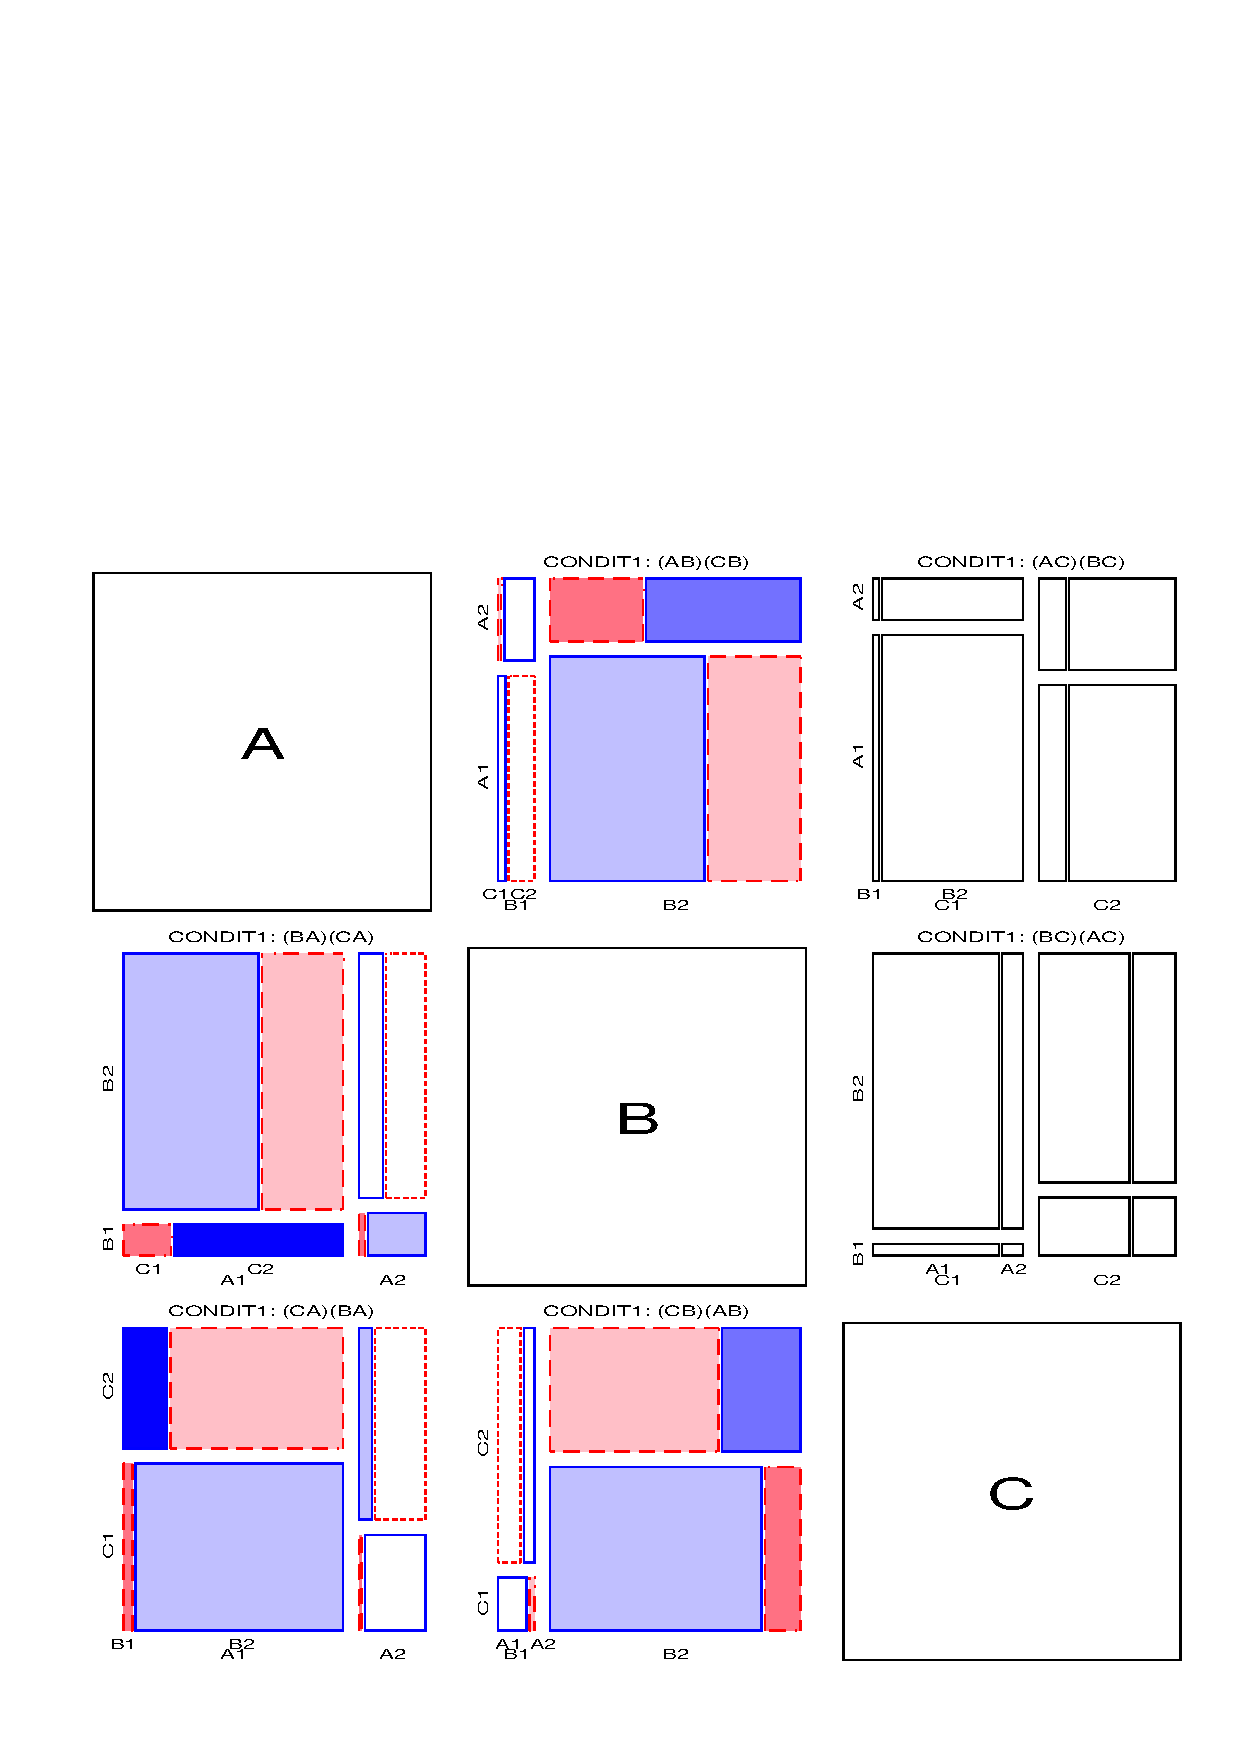
\includegraphics[scale=.6]{ch4/fig/mosfit-3}
  \caption[Mosaic matrix for conditional independence]{Mosaic matrix for conditional independence}%
  \label{fig:mosfit-3}
\end{figure}
We now see the characteristic signature of conditional independence in the
$(1, 3)$ and $(2, 3)$ panels, where $A$ and $B$ are independent at
each level of $C$. But no independence relations appear in the four
large blocks of the first two variables in any panel, so
no pair of variables is marginally independent.%
\footnote{In this data $A$ and $B$ have quite a weak association, as
may be seen in the $(1, 2)$ and $(2, 1)$ panels, where the large blocks
nearly align.}

%\section{Chapter summary}
\begin{itemize}
\item Correspondence analysis is an exploratory technique, designed to
show the row and column categories in a two- (or three-) dimensional
space.  These graphical displays, and various extensions, provide
ways to interpret the patterns of association and visually explore 
the adequacy of certain \loglin models.

\item The scores assigned to the categories of each variable are optimal
in several equivalent ways.
Among other properties,
they maximize the (canonical) correlations between the quantified
variables (weighted by cell frequencies), and make the regressions
of each variable on the other most nearly linear, for each CA dimension.

\item Multi-way tables may be analyzed in several ways.
In the ``stacking'' approach, two or more variables may be combined
interactively in the rows and/or columns of an \nway table.
Simple CA of the restructured table reveals associations between
the row and column categories of the restructured table,
but hides associations between the variables combined interactively.
Each way of stacking corresponds to a particular \loglin model
for the full table.

\item Multiple \ca is a generalization of CA to two or more variables
based on representing the data as an indicator matrix, or the Burt matrix.
The usual MCA provides an analysis of the joint, bivariate relations
between all pairs of variables.

% \item An extended form of MCA provides a means to display higher-order
% associations among multiple categorical variables.
% For $2^Q$ tables composed of $Q$ binary variables, this analysis yields
% simple geometric relations that may be interpreted in terms of odds ratios.
% \TODO{Delete this if \secref{sec:ca-mcainter} is not included.}

\item The biplot is a related technique for visualizing the elements of
a data array by points or vectors in a joint display of their row and
column categories. A standard CA biplot represents the contributions to
lack of independence as the projection of the points for rows
(or columns) on vectors for the other categories.

\item Another application of the biplot to \ctab data is described, based on analysis
of log frequency.
This analysis also serves to diagnose patterns of independence and
partial independence in two-way and larger tables.
\end{itemize}

%\section{Further reading}

